\documentclass[10pt, aspectratio=169]{beamer}

\usepackage[utf8]{inputenc}
\usepackage[T1]{fontenc}
\usepackage[polish]{babel}
\usepackage{lmodern}
\usepackage{amsmath}
\usepackage{tikz}
\usepackage{xcolor}  
\usepackage{float}   
\usepackage{newfloat}
\usepackage{fancyvrb}
\usepackage{multirow}
\usepackage{tabularx}
\usepackage{subfigure}
\usepackage{subcaption}
\usepackage{graphicx}

\usetheme{metropolis}
\metroset{block=fill} 
\setbeamertemplate{navigation symbols}{}

\definecolor{consoleGreen}{RGB}{22, 198, 12}
\definecolor{consoleRed}{RGB}{197, 15, 31}
\definecolor{consoleYellow}{RGB}{193, 156, 0}
\definecolor{consoleBlue}{RGB}{0, 55, 218}
\definecolor{consoleGray}{RGB}{100, 100, 100}
\definecolor{consolePurple}{RGB}{136, 23, 152}

\newcommand{\txtGreen}[1]{\textcolor{consoleGreen}{#1}}
\newcommand{\txtRed}[1]{\textcolor{consoleRed}{#1}}
\newcommand{\txtYellow}[1]{\textcolor{consoleYellow}{#1}}
\newcommand{\txtBlue}[1]{\textcolor{consoleBlue}{#1}}
\newcommand{\txtGray}[1]{\textcolor{consoleGray}{#1}}
\newcommand{\txtPurple}[1]{\textcolor{consolePurple}{#1}}

\newfloat{code}{H}{loc}[section]
\floatname{code}{Listing}

\title{Breakthrough}
\subtitle{Zastosowanie Monte-Carlo Tree Search do implementacji sztucznej inteligencji w grze Breakthrough}
\author{Adam Grącikowski i Piotr Iśtok}
\institute{Metody Sztucznej Inteligencji 2}
\date{15 czerwca 2026}

\begin{document}

\maketitle

\begin{frame}{Plan prezentacji}
    \tableofcontents
\end{frame}

\section{Wprowadzenie}

\begin{frame}{Zasady gry}

\begin{columns}

\begin{column}{0.5\textwidth}

\vspace{0.1cm}
\textbf{Początek gry:}
\begin{itemize}
    \item Każdy gracz ma 16 pionów.
    \item Piony ustawione są na dwóch skrajnych rzędach planszy.
\end{itemize}

\vspace{0.1cm}

\textbf{Ruchy:}
\begin{itemize}
    \item Ruch o jedno pole do przodu lub po skosie do przodu.
    \item Bicie tylko po skosie do przodu.
    \item Brak ruchu i bicia do tyłu oraz w poziomie.
\end{itemize}

\vspace{0.1cm}

\textbf{Warunki zwycięstwa:}
\begin{itemize}
    \item Dotarcie pionem do ostatniego rzędu przeciwnika (ang. \textit{breakthrough}).
    \item Zbicie wszystkich pionów przeciwnika.
\end{itemize}

\end{column}

\begin{column}{0.40\textwidth}
    \centering
    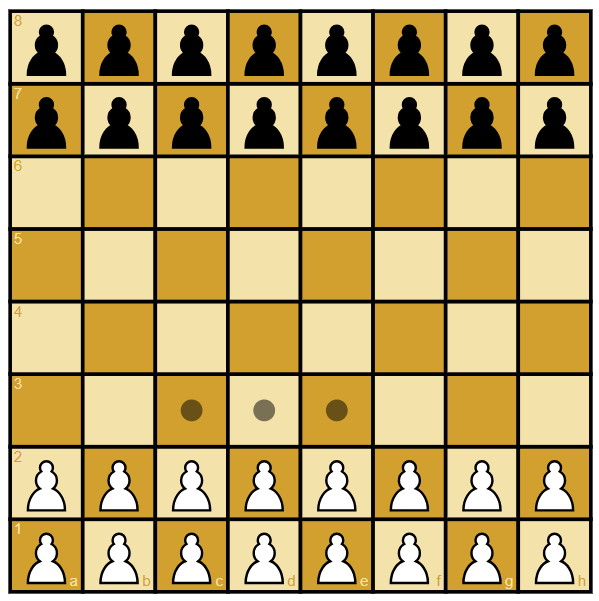
\includegraphics[width=\textwidth]{images/board_example.png}

    \vspace{0.1cm}
    {\scriptsize Stan planszy na początku gry}
\end{column}

\end{columns}

\end{frame}

\begin{frame}{Reprezentacja stanu gry}

\begin{columns}[T]

\begin{column}{0.55\textwidth}

    \structure{\textbf{Stan planszy}} \\
    \vspace{0.1cm}
    Zamodelowany przy pomocy \textbf{tablic bitowych}:
    \begin{itemize}
        \item pełny układ bierek zapisany na 2 zmiennych bez znaku o rozmiarze 128 bitów (\texttt{u128})
        \item \textbf{bit = 1} $\rightarrow$ pion na polu
        \item \textbf{bit = 0} $\rightarrow$ puste pole
    \end{itemize}

    \vspace{0.2cm}
    
    \structure{\textbf{Kontekst rozgrywki}}
    \vspace{0.1cm}
    \begin{itemize}
        \item znacznik aktualnego gracza
        \item brak dodatkowych flag (jak w szachach)
    \end{itemize}

    \vspace{0.2cm}
    
    \textbf{Rozmiar struktury:} 33 bajty

\end{column}

\begin{column}{0.40\textwidth}
    
    \structure{\textbf{Zalety}}
    \vspace{0.1cm}
    \begin{itemize}
        \item wysoka wydajność operacji bitowych (AND/OR/XOR)
        \item mały rozmiar i narzut pamięciowy
        \item masowe przetwarzanie stanów
    \end{itemize}
    
    \vspace{0.5cm}
    
    \structure{\textbf{Ograniczenia}}
    \vspace{0.1cm}
    \begin{itemize}
        \item pojemność do maksymalnie \\ 128 pól
        \item w praktyce plansza do $11 \times 11$
    \end{itemize}

\end{column}

\end{columns}

\end{frame}

\section{Algorytmy}

\begin{frame}{Zaimplementowane algorytmy}
    \begin{itemize}
        \item \textbf{Minimax} (agent heurystyczny)
        \item \textbf{MCTS}~\cite{coulom2006efficient, kocsis2006bandit}
        \item \textbf{MCTS + RAVE}~\cite{gelly2007monte, sutton2018reinforcement}
        \item \textbf{MCTS + Heavy Playouts}~\cite{browne2012survey}
    \end{itemize}
\end{frame}

\begin{frame}{Agent Minimax}

    \begin{columns}[T]
    \begin{column}{0.5\textwidth}
        \structure{\textbf{Przeszukiwanie drzewa gry}}
        \vspace{0.1cm}
        \begin{itemize}
            \item Zastosowanie klasycznego algorytmu \textbf{Minimax} z \textbf{odcięciami Alfa-Beta} \\ (ang. \textit{Alpha-Beta pruning}).
            \item Ograniczenie głębokości i deterministyczne działanie w oparciu o funkcję oceny pozycji $E$.
        \end{itemize}
    \end{column}
    
    \begin{column}{0.45\textwidth}
        \structure{\textbf{Kryteria oceny pozycji}}
        \vspace{0.1cm}
        \begin{itemize}
            \item Zaawansowanie pionów.
            \item Przewaga materialna.
            \item Struktury obronne.
            \item Kara za grę kolumnami \texttt{A} i \texttt{H} \\(piony mają tam tylko dwie opcje ruchu zamiast trzech).
        \end{itemize}
    \end{column}
    
    \end{columns}

    \vspace{0.6cm}
    
    \structure{\textbf{Proces decyzyjny}} \\
    Podobnie jak ludzie planuje swoje akcje kilka kroków w przód, a następnie intuicyjnie ocenia ($\max \{E(s_t):~s_t \in S_t\}$), czy powstała w ten sposób sytuacja na planszy jest dla niego korzystna.

\end{frame}

\begin{frame}{MCTS}
    \begin{columns}[T]
    \begin{column}{0.50\textwidth}
        \structure{\textbf{Idea}}
        \vspace{0.1cm}
        \begin{itemize}
            \item Probabilistyczne przeszukiwanie drzewa gry~\cite{coulom2006efficient}.
            \item Drzewo rozwijane asymetrycznie -- więcej iteracji trafia do obiecujących wariantów.
            \item Węzeł przechowuje stan planszy, gracza oraz statystyki odwiedzin i zwycięstw.
        \end{itemize}
    \end{column}

    \begin{column}{0.45\textwidth}
        \structure{\textbf{Jedna iteracja}}
        \vspace{0.1cm}
        \begin{enumerate}
            \item Selekcja
            \item Ekspansja
            \item Symulacja
            \item Propagacja wsteczna
        \end{enumerate}
    \end{column}
    \end{columns}

    \vspace{0.45cm}

    \structure{\textbf{Selekcja UCB1}}~\cite{kocsis2006bandit}
    \[
        \frac{w_i}{n_i} + C \sqrt{\frac{\ln N}{n_i}}
    \]
    \small
    Eksploatacja dobrych ruchów jest równoważona eksploracją rzadziej odwiedzonych gałęzi.
\end{frame}

\begin{frame}{MCTS + RAVE}
    \begin{columns}[T]
    \begin{column}{0.50\textwidth}
        \structure{\textbf{AMAF}}~\cite{gelly2007monte}
        \vspace{0.1cm}
        \begin{itemize}
            \item RAVE przyspiesza uczenie statystyk na początku przeszukiwania~\cite{gelly2007monte}.
            \item Ruch zagrany później w symulacji traktujemy tak, jakby mógł być wartościowy także wcześniej.
            \item Oprócz statystyk MCTS przechowujemy statystyki AMAF: $\tilde{w}_i$, $\tilde{n}_i$.
        \end{itemize}
    \end{column}

    \begin{column}{0.45\textwidth}
        \structure{\textbf{Połączenie ocen}}
        \[
            V_{RAVE} =
            (1-\beta)\frac{w_i}{n_i}
            + \beta\frac{\tilde{w}_i}{\tilde{n}_i}
        \]

        \[
            \beta = \frac{k}{k+n_i}
        \]
    \end{column}
    \end{columns}

    \vspace{0.3cm}

    \small
    Gdy węzeł ma mało odwiedzin, większą rolę ma szybka estymacja AMAF. Wraz ze wzrostem $n_i$ algorytm przechodzi do klasycznej oceny UCT.
\end{frame}

\begin{frame}{MCTS + Heavy Playouts}
    \begin{columns}[T]
    \begin{column}{0.52\textwidth}
        \structure{\textbf{Problem klasycznego rollout'u}}
        \vspace{0.1cm}
        \begin{itemize}
            \item Standardowy MCTS symuluje partię losowymi ruchami.
            \item W Breakthrough losowe symulacje często tworzą mało realistyczne przebiegi.
            \item Heavy Playouts kierują symulację wiedzą dziedzinową~\cite{browne2012survey}.
        \end{itemize}
    \end{column}

    \begin{column}{0.43\textwidth}
        \structure{\textbf{Polityka $\epsilon$-greedy}}~\cite{sutton2018reinforcement}
        \vspace{0.1cm}
        \begin{itemize}
            \item z prawdopodobieństwem $\epsilon$ ruch losowy,
            \item z prawdopodobieństwem $1-\epsilon$ najlepszy ruch według $E$.
        \end{itemize}
    \end{column}
    \end{columns}

    \vspace{0.45cm}

    \structure{\textbf{Funkcja oceny}} \\
    W symulacjach wykorzystywana jest ta sama funkcja heurystyczna $E$, co w agencie Minimax: przewaga materialna, zaawansowanie pionów, struktury obronne oraz kara za grę krawędzią.

    \vspace{0.25cm}
    \small
    Cena tej modyfikacji to większy koszt obliczeniowy każdej symulacji.
\end{frame}

\section{Konfiguracja eksperymentów}

\begin{frame}[fragile]{Format pliku wejściowego}
    \begin{columns}
        \begin{column}{0.55\textwidth}
            \scriptsize
            \begin{Verbatim}[commandchars=\|\{\}]
board_width = |txtBlue{6}
board_height = |txtBlue{7}
seed = |txtBlue{100}

|txtPurple{[white_player]}
type = |txtYellow{"Minimax"}
max_depth = |txtBlue{5}
material_weight = |txtBlue{250}
advancement_weight = |txtBlue{10}

|txtPurple{[black_player]}
type = |txtYellow{"Mcts"}
max_iterations = |txtBlue{100000}
exploration_constant = |txtBlue{1.41}
use_heavy_playouts = |txtRed{true}
            \end{Verbatim}
            \vspace{0.5cm}
            \normalsize
            { Przykładowy plik konfiguracyjny.}
        \end{column}

        \begin{column}{0.45\textwidth}
            \textbf{Charakterystyka:}
            \begin{itemize}
                \item Konfiguracja graczy w formacie TOML.
                \item Brakujące pola uzupełniane wartościami domyślnymi.
            \end{itemize}
        \end{column}
    \end{columns}
\end{frame}

\begin{frame}{Konfiguracja agenta Minimax}

\renewcommand{\arraystretch}{1.2}

\begin{table}
\centering
\caption{Pola konfiguracyjne dla agenta typu Minimax.}
\scriptsize
\begin{tabularx}{0.8\textwidth}{|
    >{\raggedright\arraybackslash}m{2.5cm}|
    >{\centering\arraybackslash}m{1.5cm}|
    >{\raggedright\arraybackslash}X|}
    \hline
    \textbf{Pole} & \textbf{Domyślnie} & \textbf{Opis} \\
    \hline
    \texttt{max\_depth} & 4 &
    Maksymalna głębokość przeszukiwania drzewa gry. \\
    \hline
    \texttt{material\_weight} & 200 &
    Waga przewagi materialnej (liczby bierek). \\
    \hline
    \texttt{advancement\_weight} & 5 &
    Premia za zaawansowanie pionów w kierunku celu przeciwnika. \\
    \hline
    \texttt{defended\_weight} & 5 &
    Premia za wzajemnie broniące się piony. \\
    \hline
    \texttt{edge\_penalty\_weight} & -2 &
    Kara za ustawianie pionów na krawędziach planszy. \\
    \hline
\end{tabularx}
\end{table}

\end{frame}

\begin{frame}{Konfiguracja agenta MCTS}

\small
\renewcommand{\arraystretch}{1.1}

\begin{table}
\centering
\caption{Pola konfiguracyjne dla agenta typu MCTS.}
\scriptsize
\begin{tabularx}{0.8\textwidth}{|
    >{\raggedright\arraybackslash}m{3cm}|
    >{\centering\arraybackslash}m{1.5cm}|
    >{\raggedright\arraybackslash}X|}
    \hline
    \textbf{Pole} & \textbf{Domyślnie} & \textbf{Opis} \\
    \hline
    \texttt{max\_iterations} & 75000 &
    Maksymalna liczba iteracji algorytmu MCTS. \\
    \hline
    \texttt{max\_time\_ms} & None &
    Limit czasu na ruch (ms). Nadpisuje liczbę iteracji. \\
    \hline
    \texttt{exploration\_constant} & 1.41 &
    Stała eksploracji ($C$) w formule UCT. \\
    \hline
    \texttt{use\_rave} & false &
    Aktywuje modyfikację RAVE. \\
    \hline
    \texttt{rave\_k} & 1000.0 &
    Waga heurystyki RAVE w stosunku do UCT. \\
    \hline
    \texttt{use\_heavy\_playouts} & false &
    Aktywuje symulacje kierowane heurystyką. \\
    \hline
    \texttt{heavy\_playouts\_epsilon} & 0.1 &
    Szansa na losowy ruch ($\varepsilon$) w ulepszonych symulacjach. \\
    \hline
    \texttt{material\_weight} & 200 &
    Waga przewagi materialnej. \\
    \hline
    \texttt{advancement\_weight} & 5 &
    Waga zaawansowania pionów. \\
    \hline
    \texttt{defended\_weight} & 5 &
    Premia za bronione piony. \\
    \hline
    \texttt{edge\_penalty\_weight} & -2 &
    Kara za piony na krawędzi. \\
    \hline
\end{tabularx}
\end{table}

\end{frame}

\section{Wyniki eksperymentów}

\begin{frame}{Przewaga wariantów MCTS nad Minimax}
    \textbf{Metodologia:}
    \begin{itemize}
        \item 3 warianty: MCTS, MCTS + RAVE, MCTS + Heavy Playouts
        \item Oponent: Minimax z głębokością $d \in [1,7]$
        \item 20 partii na każdą głębokość (10 białe, 10 czarne)
        \item Łącznie: 420 gier
        \item Stały budżet MCTS: 10000 iteracji
    \end{itemize}
    \textbf{Metryki:}
    \begin{itemize}
        \item Współczynnik zwycięstw
        \item Średnia długość gry
        \item Czas decyzji
    \end{itemize}
\end{frame}

\begin{frame}{Współczynnik zwycięstw}
    \centering
    \begin{minipage}{0.30\textwidth}
        \centering
        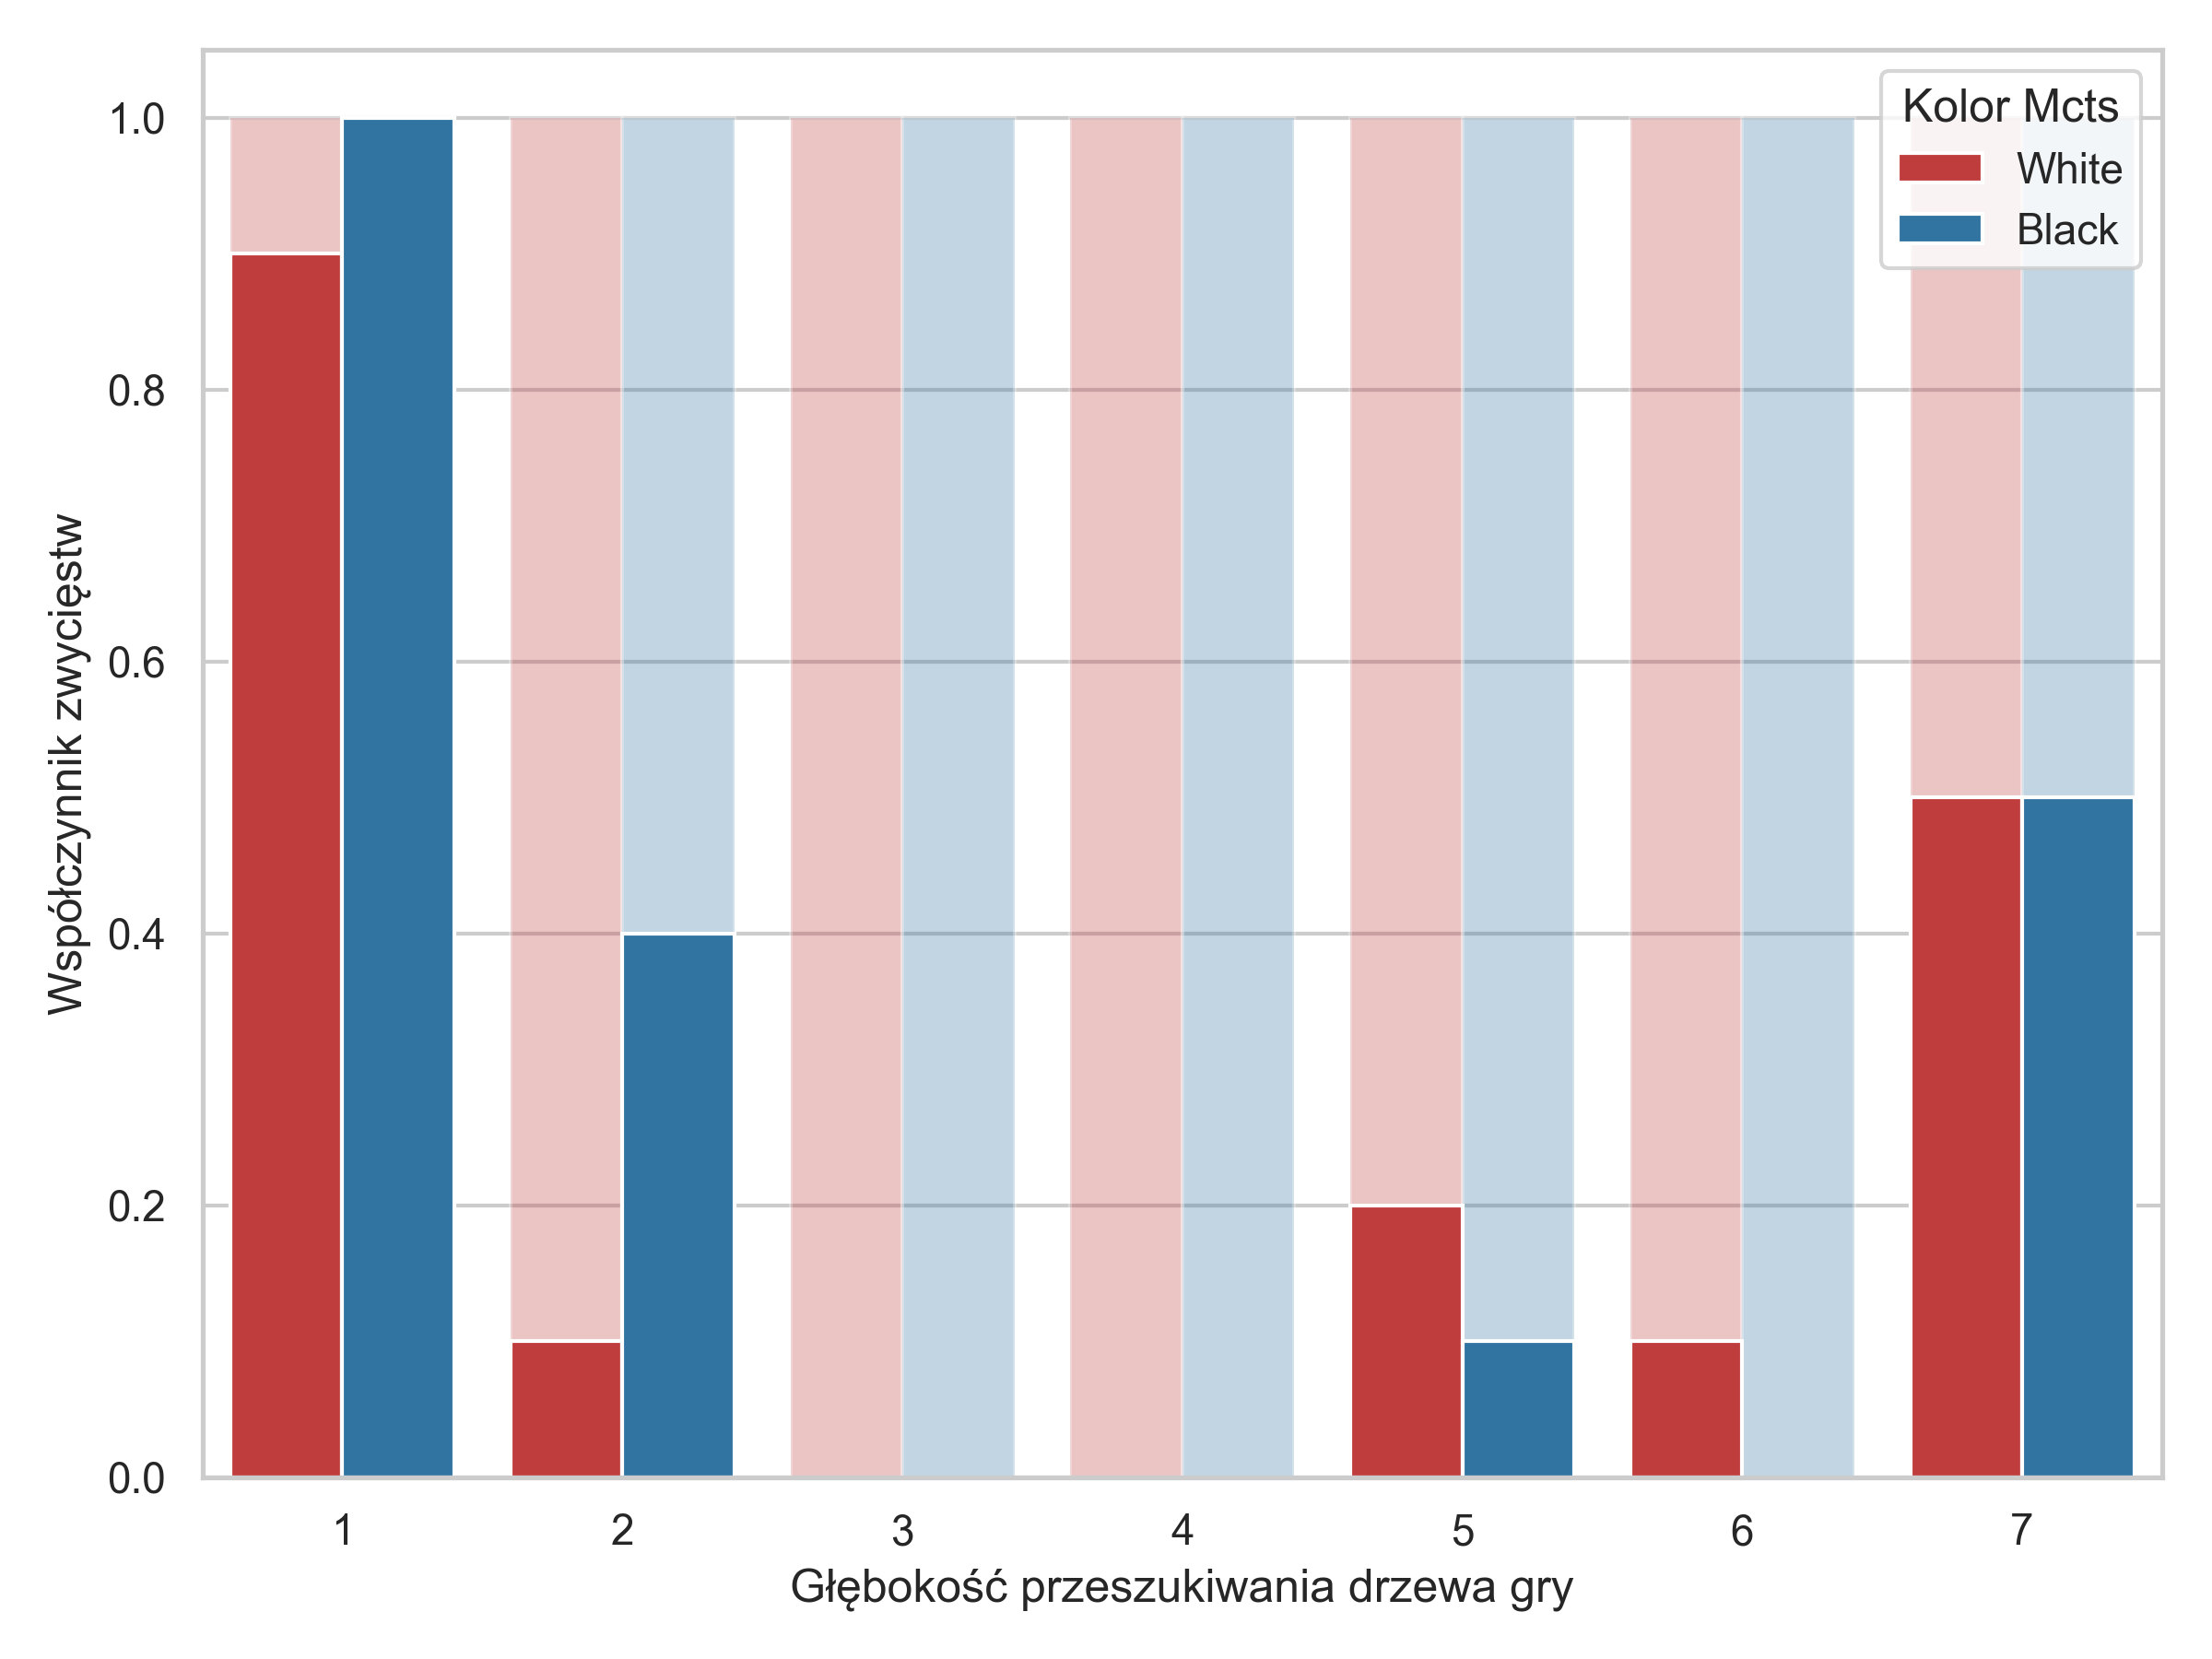
\includegraphics[width=\textwidth]{images/mcts_win_rate.png}\\
        {\scriptsize MCTS}
    \end{minipage}%
    \hfill
    \begin{minipage}{0.30\textwidth}
        \centering
        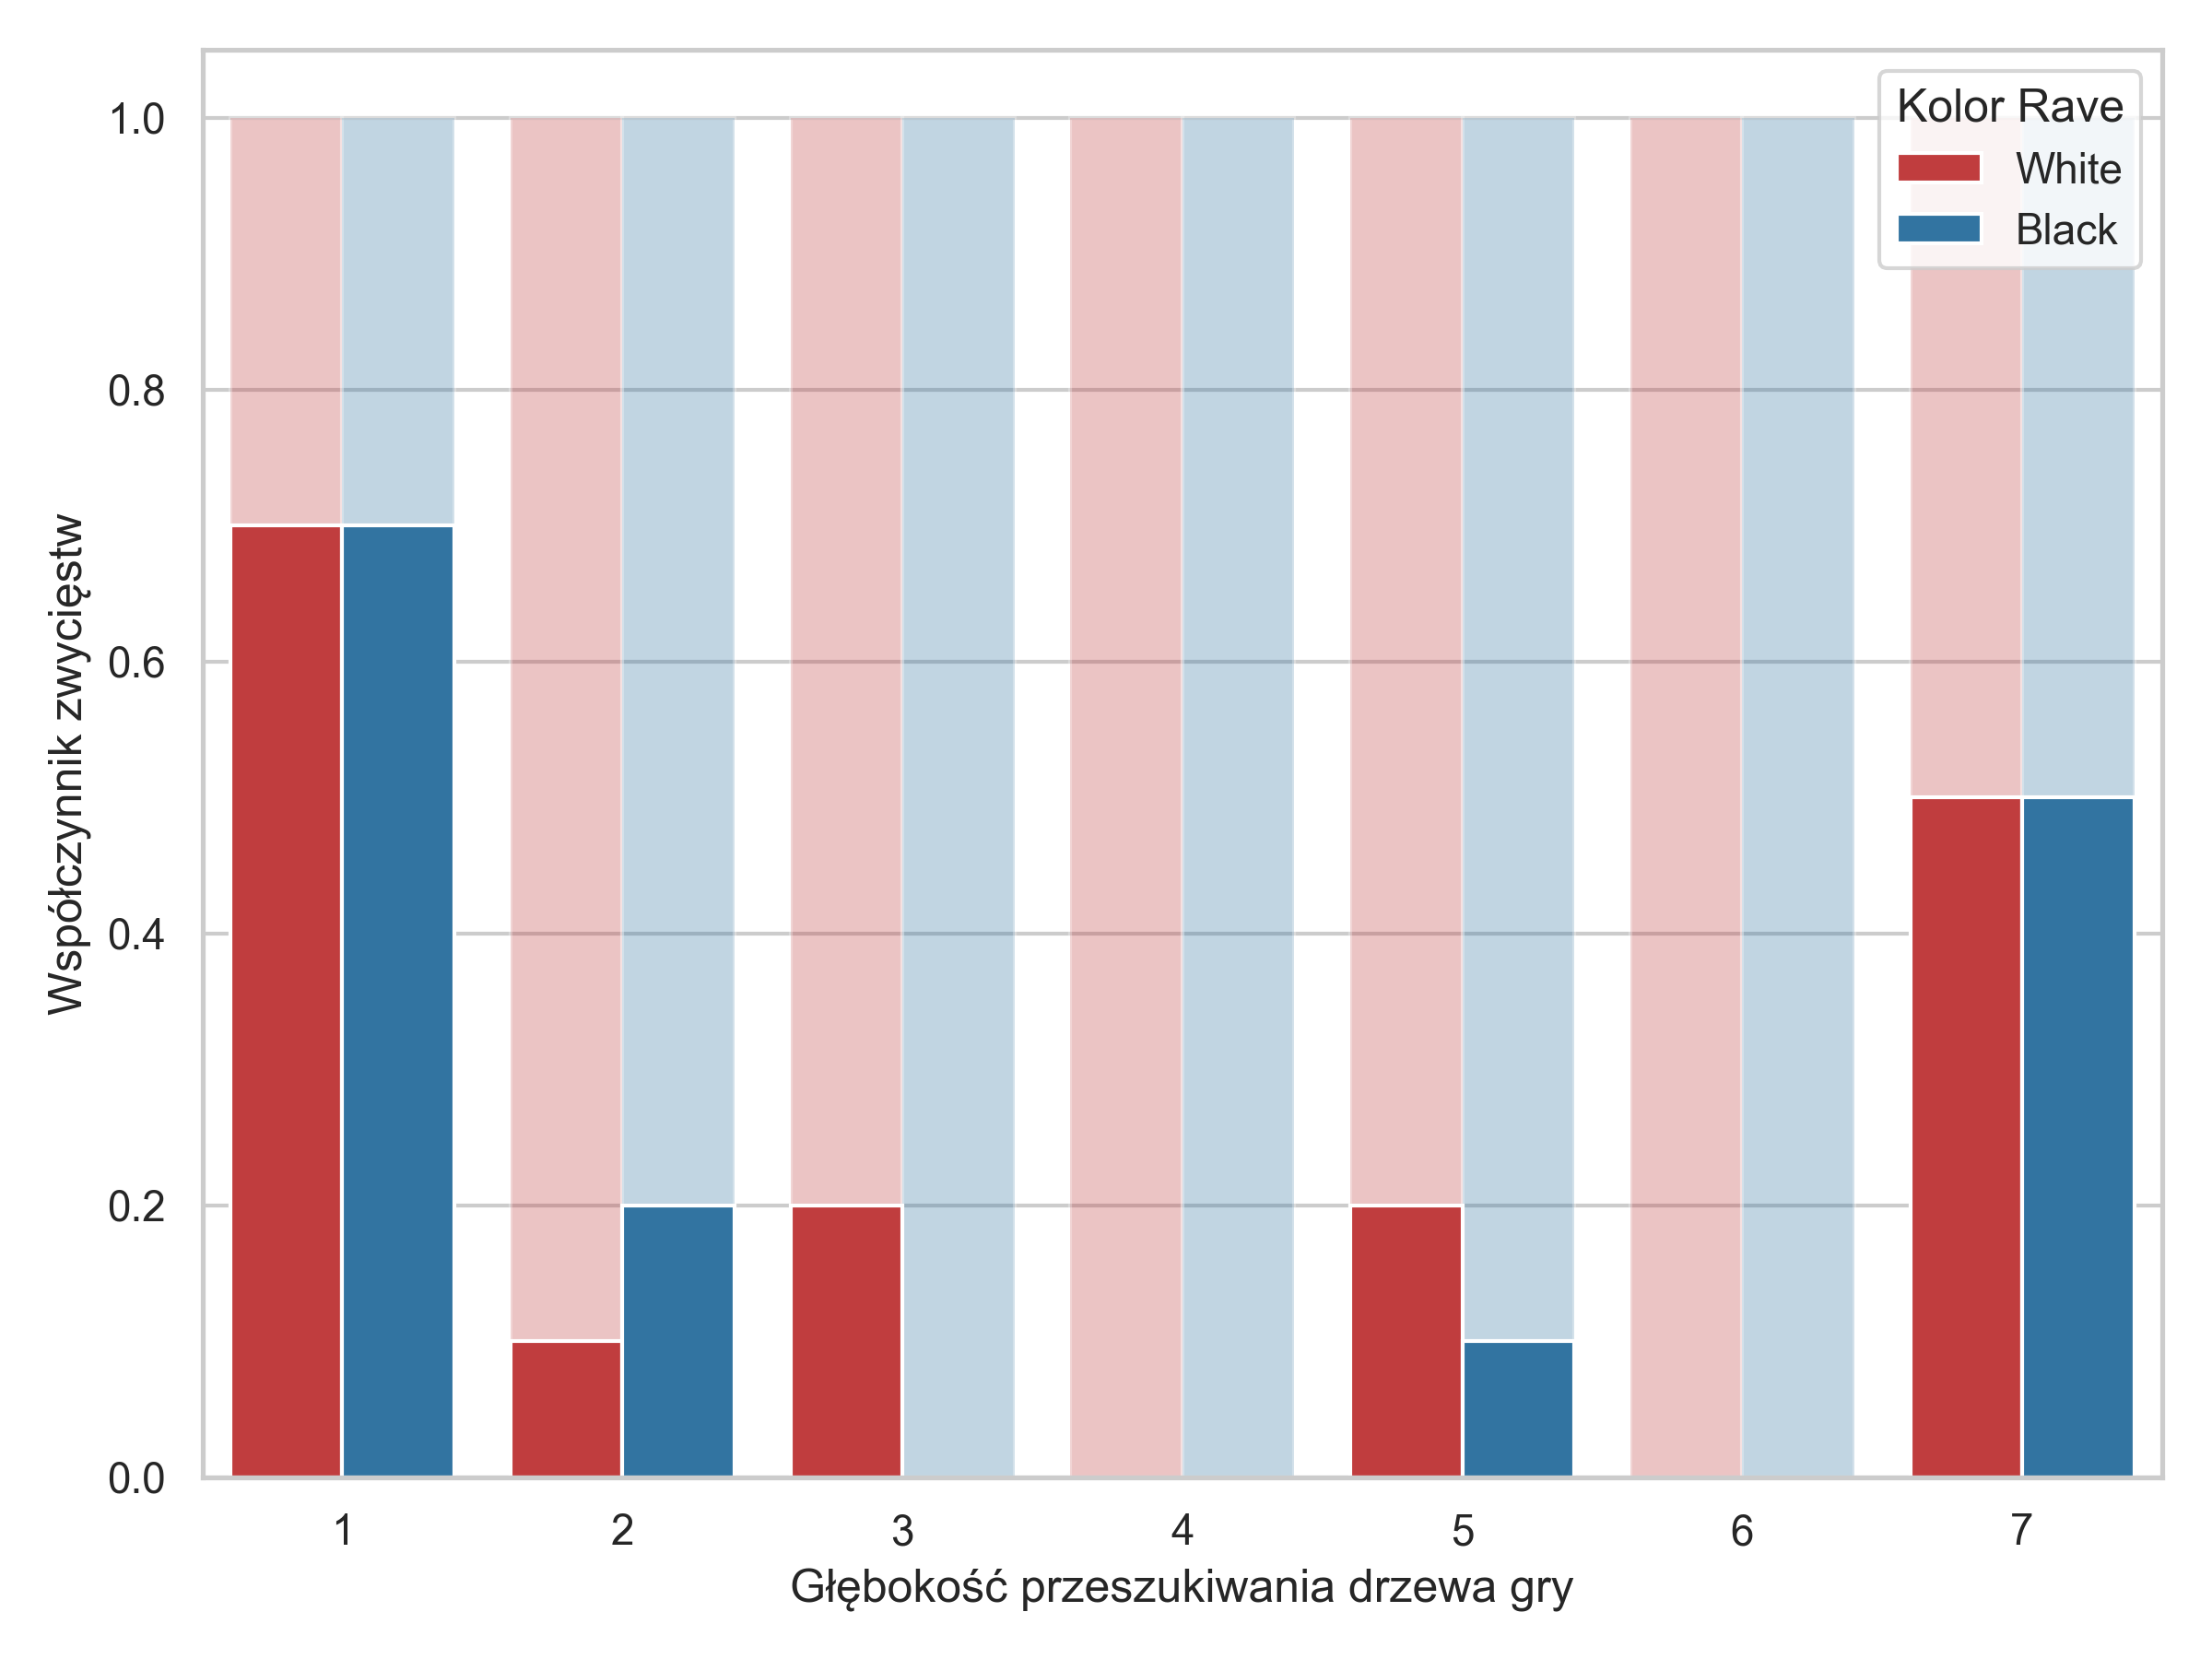
\includegraphics[width=\textwidth]{images/rave_win_rate.png}\\
        {\scriptsize MCTS + RAVE}
    \end{minipage}%
    \hfill
    \begin{minipage}{0.30\textwidth}
        \centering
        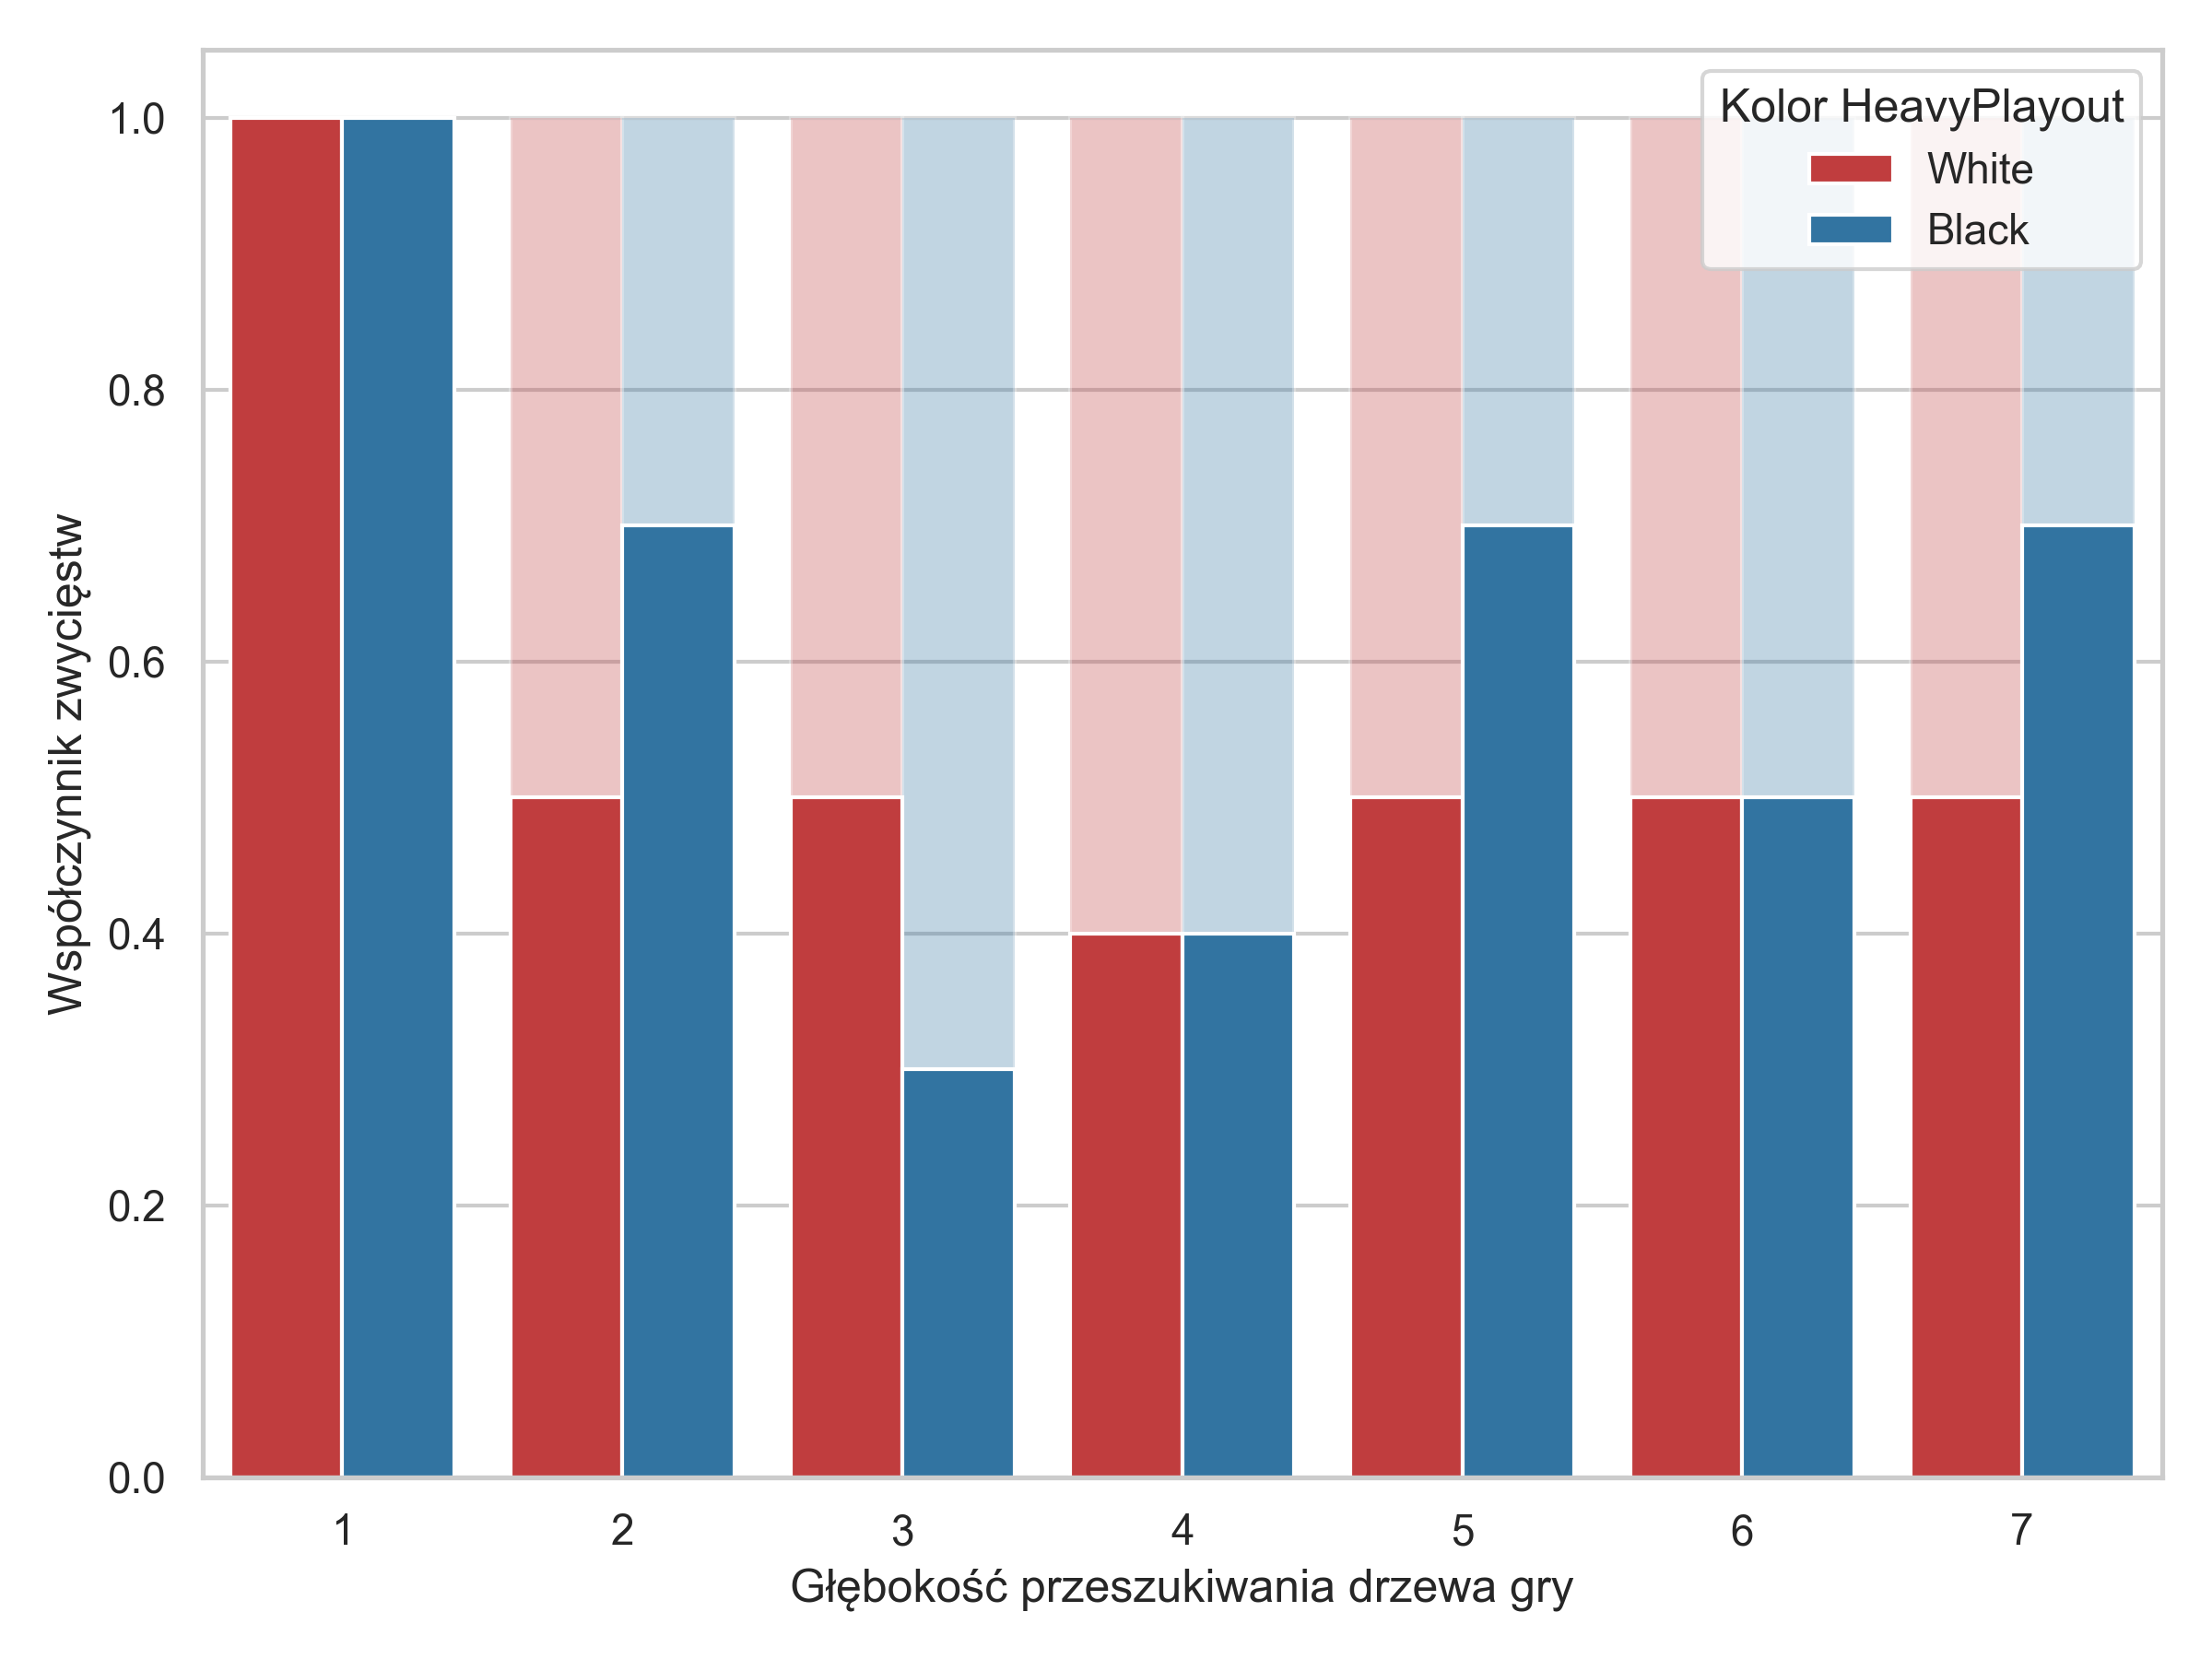
\includegraphics[width=\textwidth]{images/heavyplayouts_win_rate.png}\\
        {\scriptsize MCTS + Heavy Playouts}
    \end{minipage}
    
    \vspace{0.7cm}
    
    Porównanie odsetka wygranych partii w zależności od głębokości przeszukiwania agenta Minimax dla różnych wariantów algorytmu MCTS.
\end{frame}

\begin{frame}{Całkowita liczba ruchów}
    \centering
    \begin{minipage}{0.30\textwidth}
        \centering
        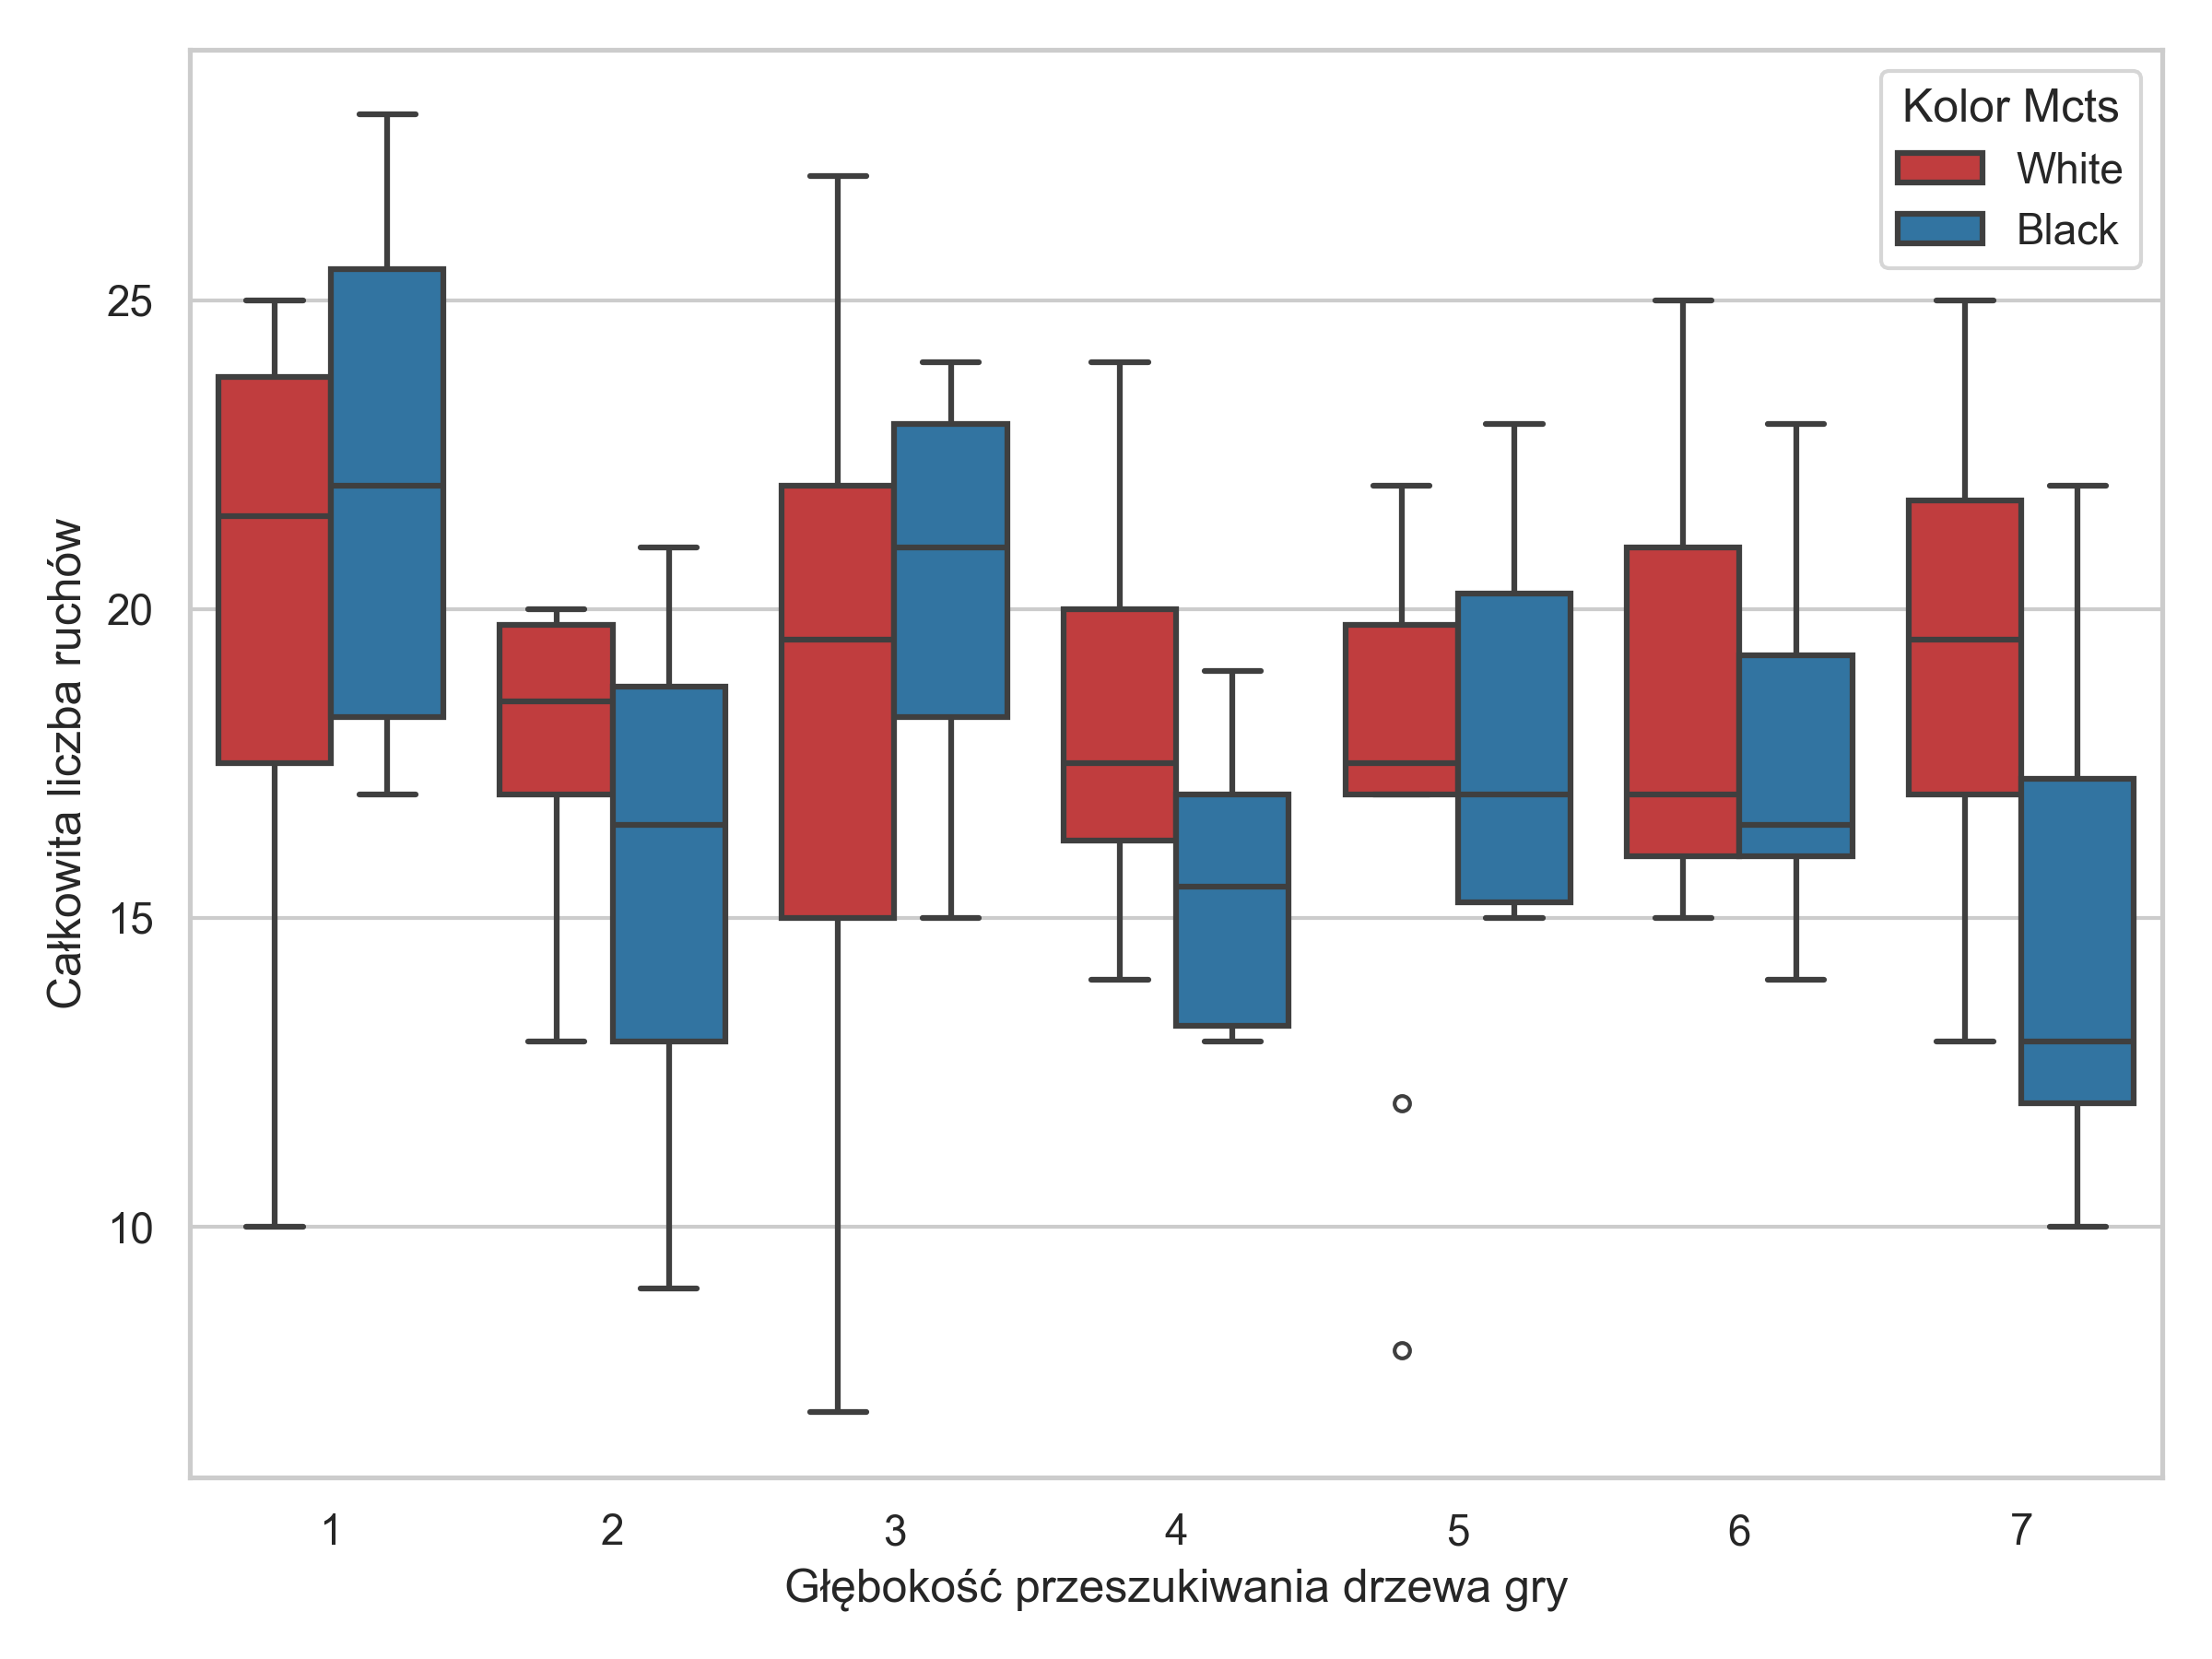
\includegraphics[width=\textwidth]{images/mcts_total_moves.png}\\
        {\scriptsize MCTS}
    \end{minipage}%
    \hfill
    \begin{minipage}{0.30\textwidth}
        \centering
        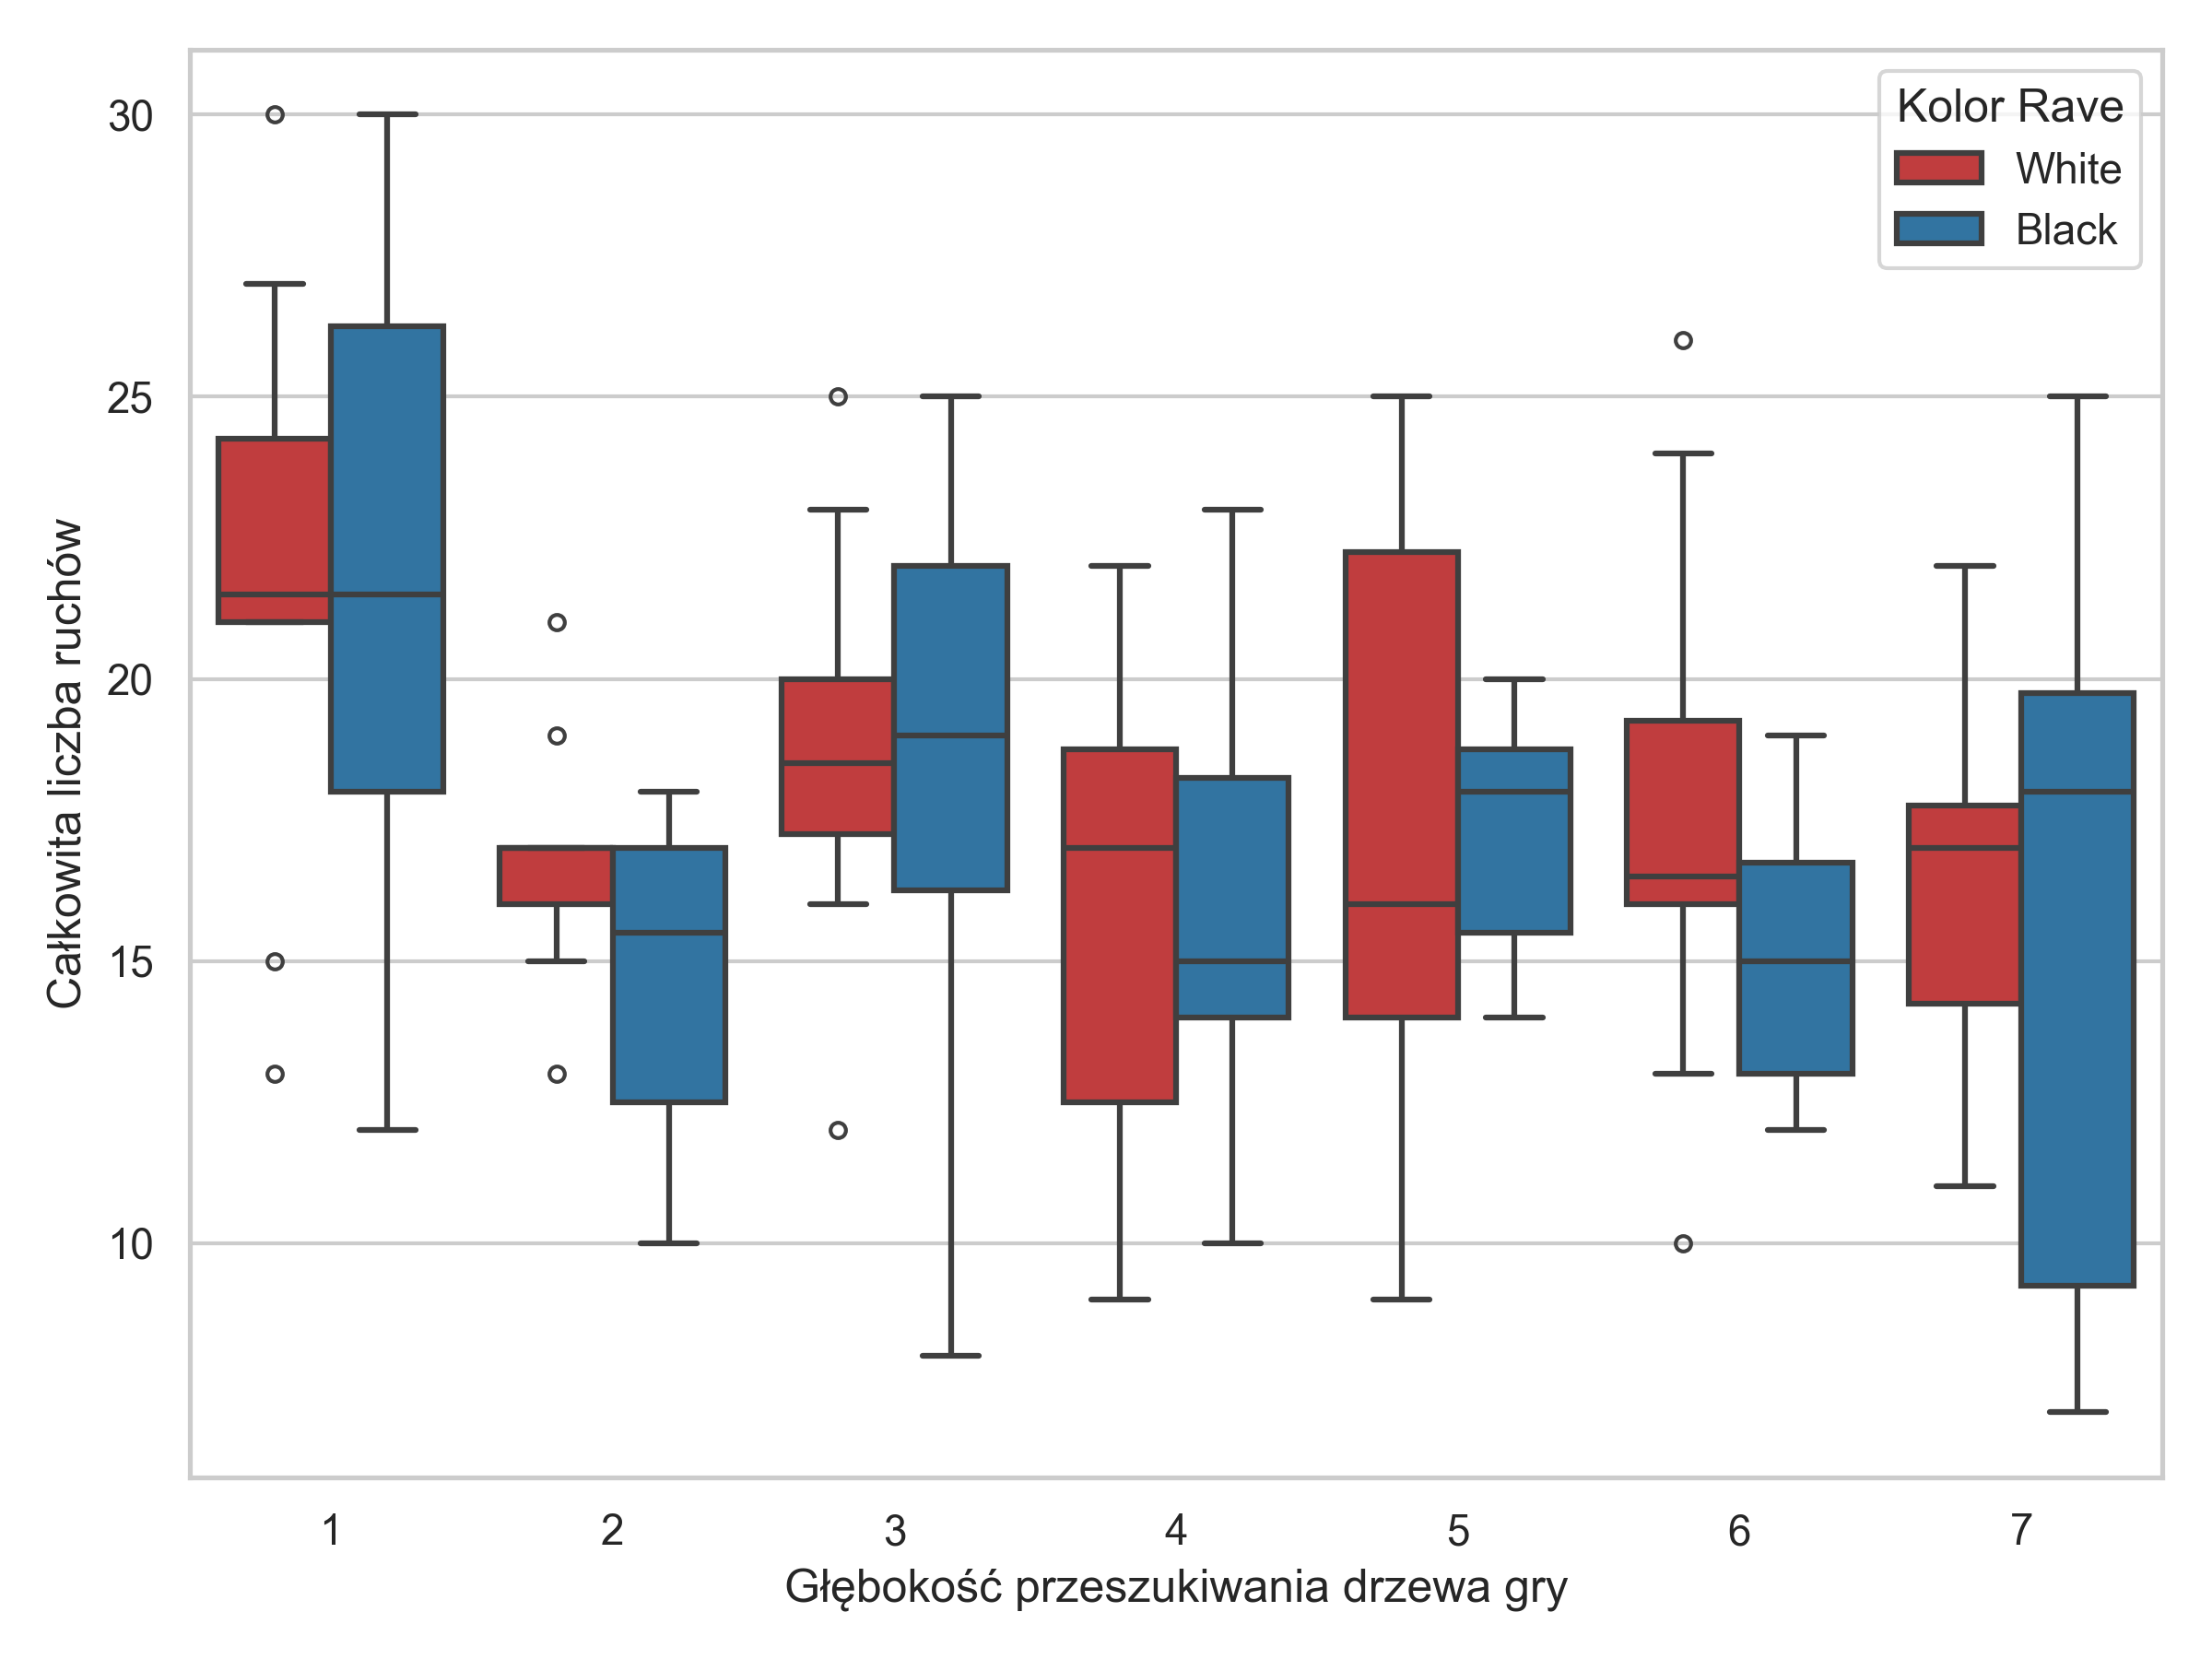
\includegraphics[width=\textwidth]{images/rave_total_moves.png}\\
        {\scriptsize MCTS + RAVE}
    \end{minipage}%
    \hfill
    \begin{minipage}{0.30\textwidth}
        \centering
        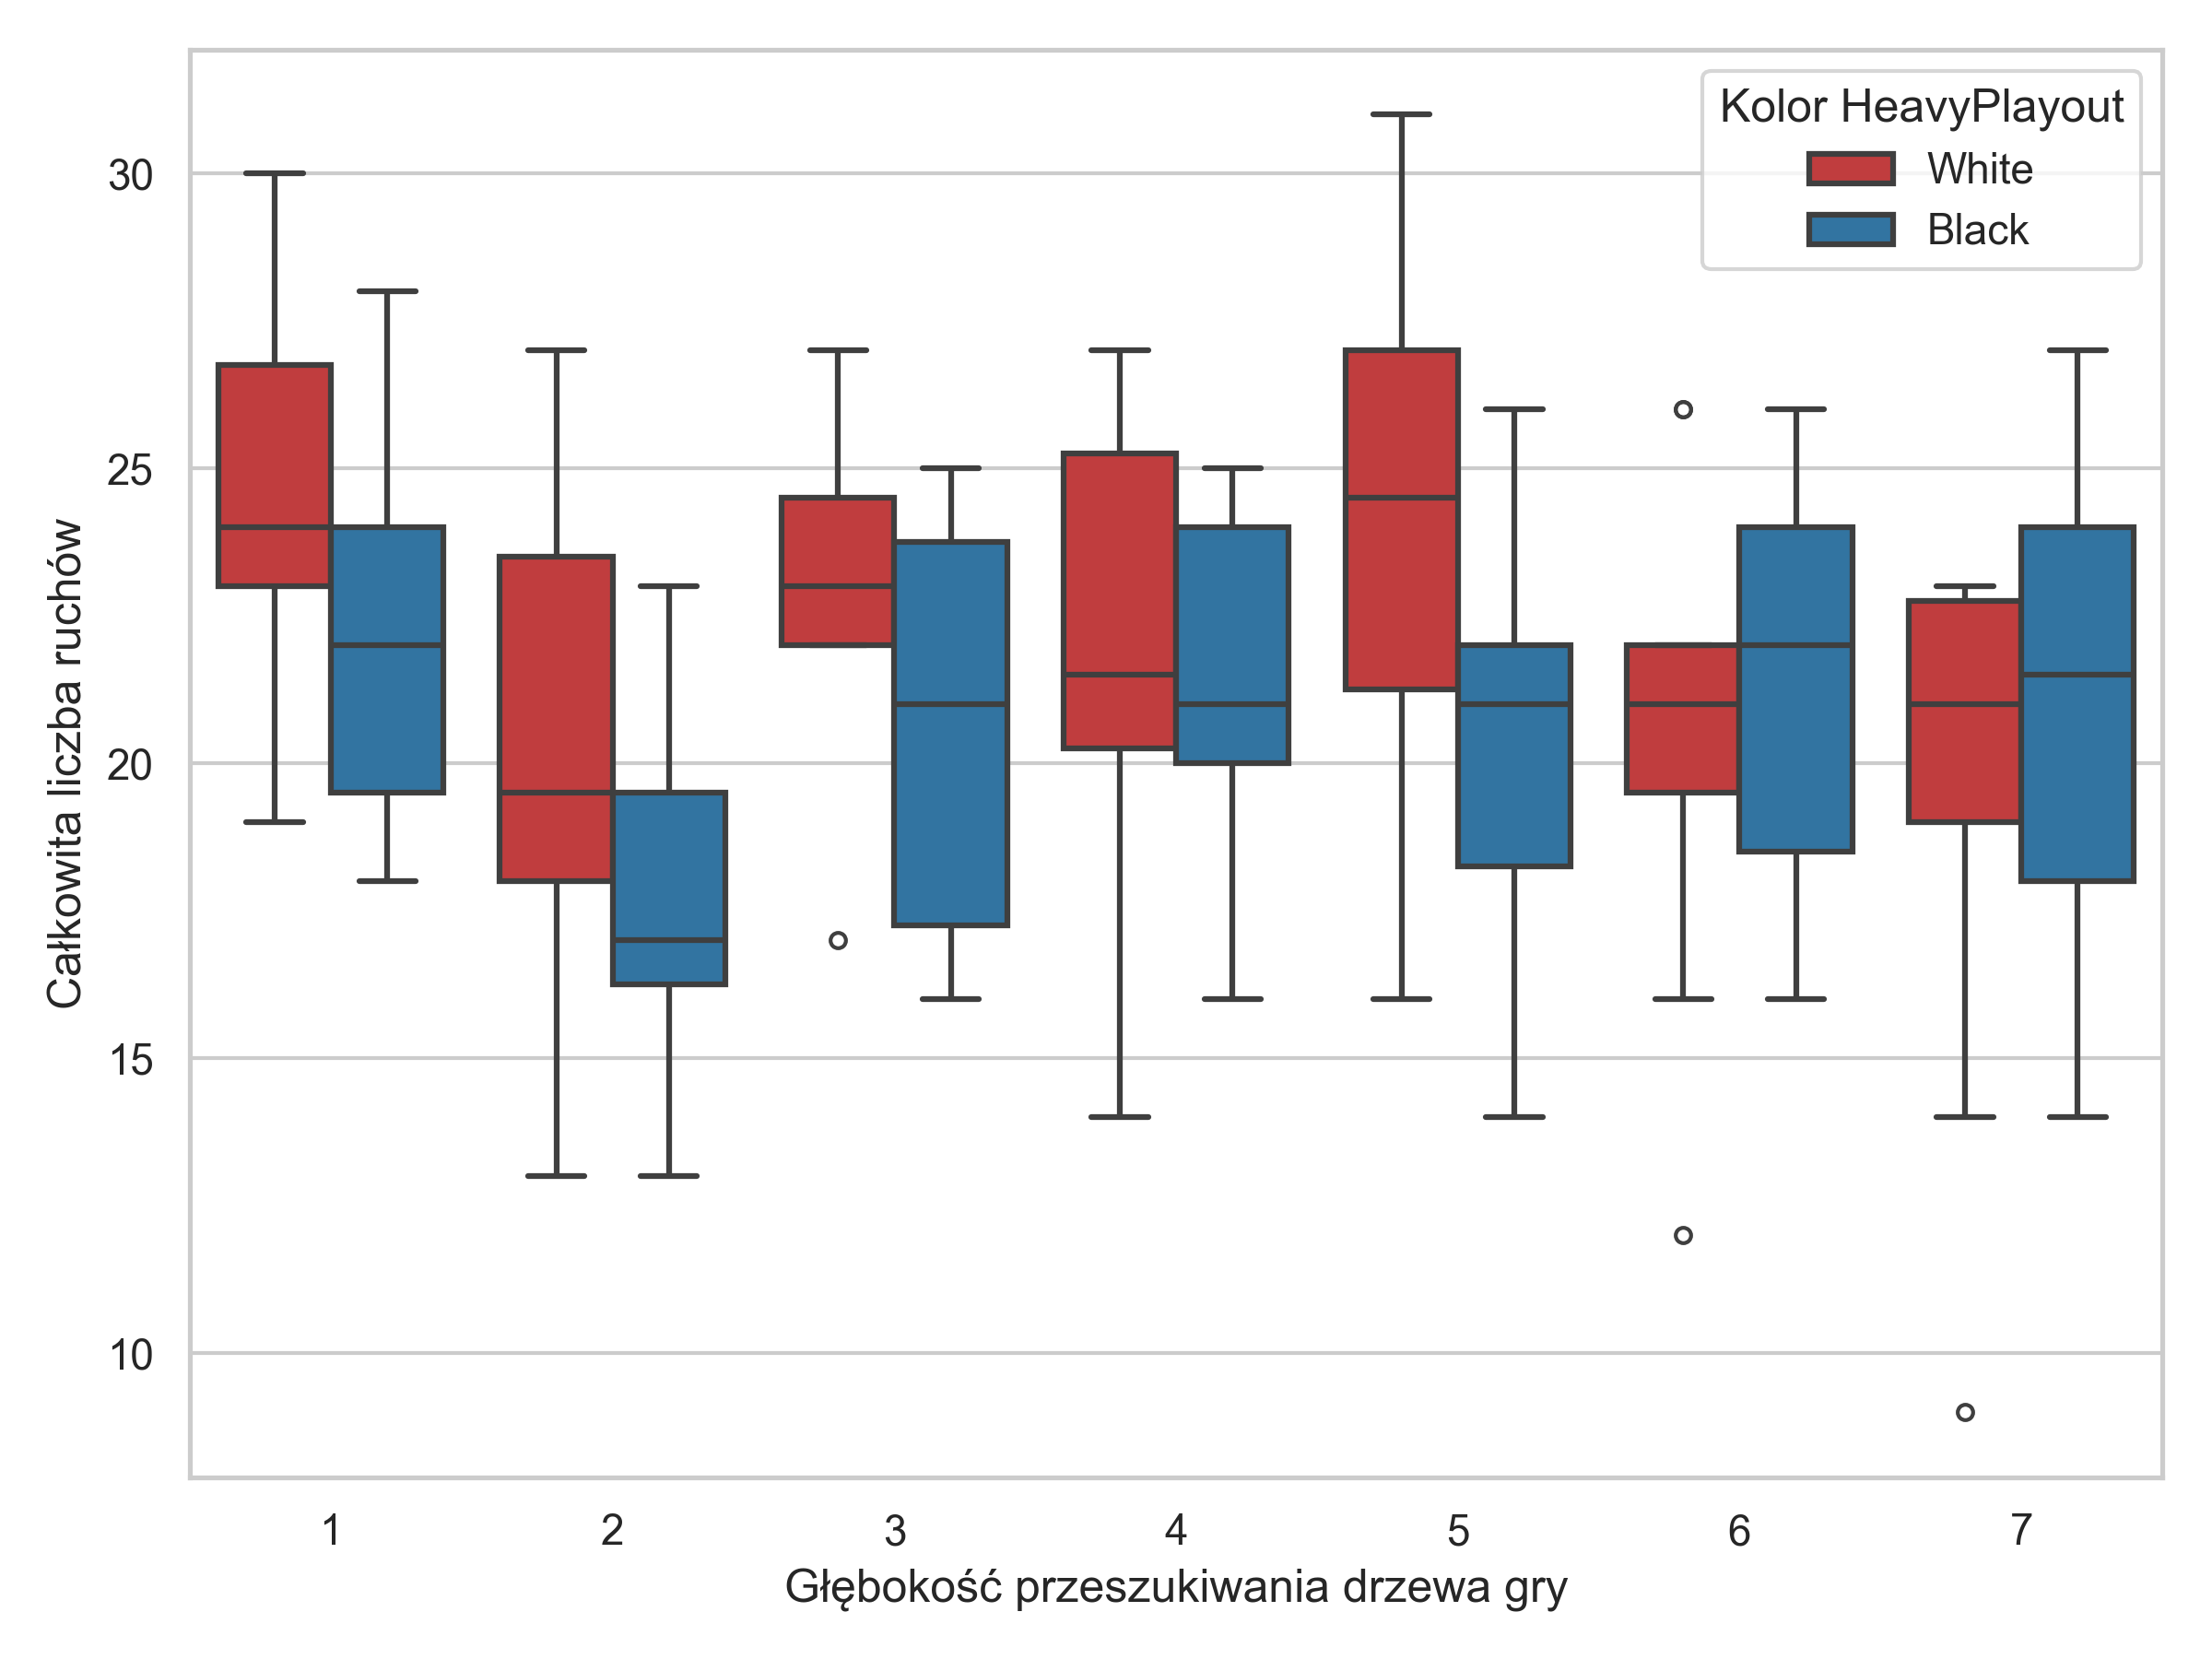
\includegraphics[width=\textwidth]{images/heavyplayouts_total_moves.png}\\
        {\scriptsize MCTS + Heavy Playouts}
    \end{minipage}
    
    \vspace{0.7cm}
    
    Zestawienie dystrybucji całkowitej liczby ruchów rozegranych w partiach przeciwko agentowi Minimax dla różnych wariantów algorytmu MCTS.
\end{frame}

\begin{frame}{Średni czas namysłu}
    \centering
    \begin{minipage}{0.30\textwidth}
        \centering
        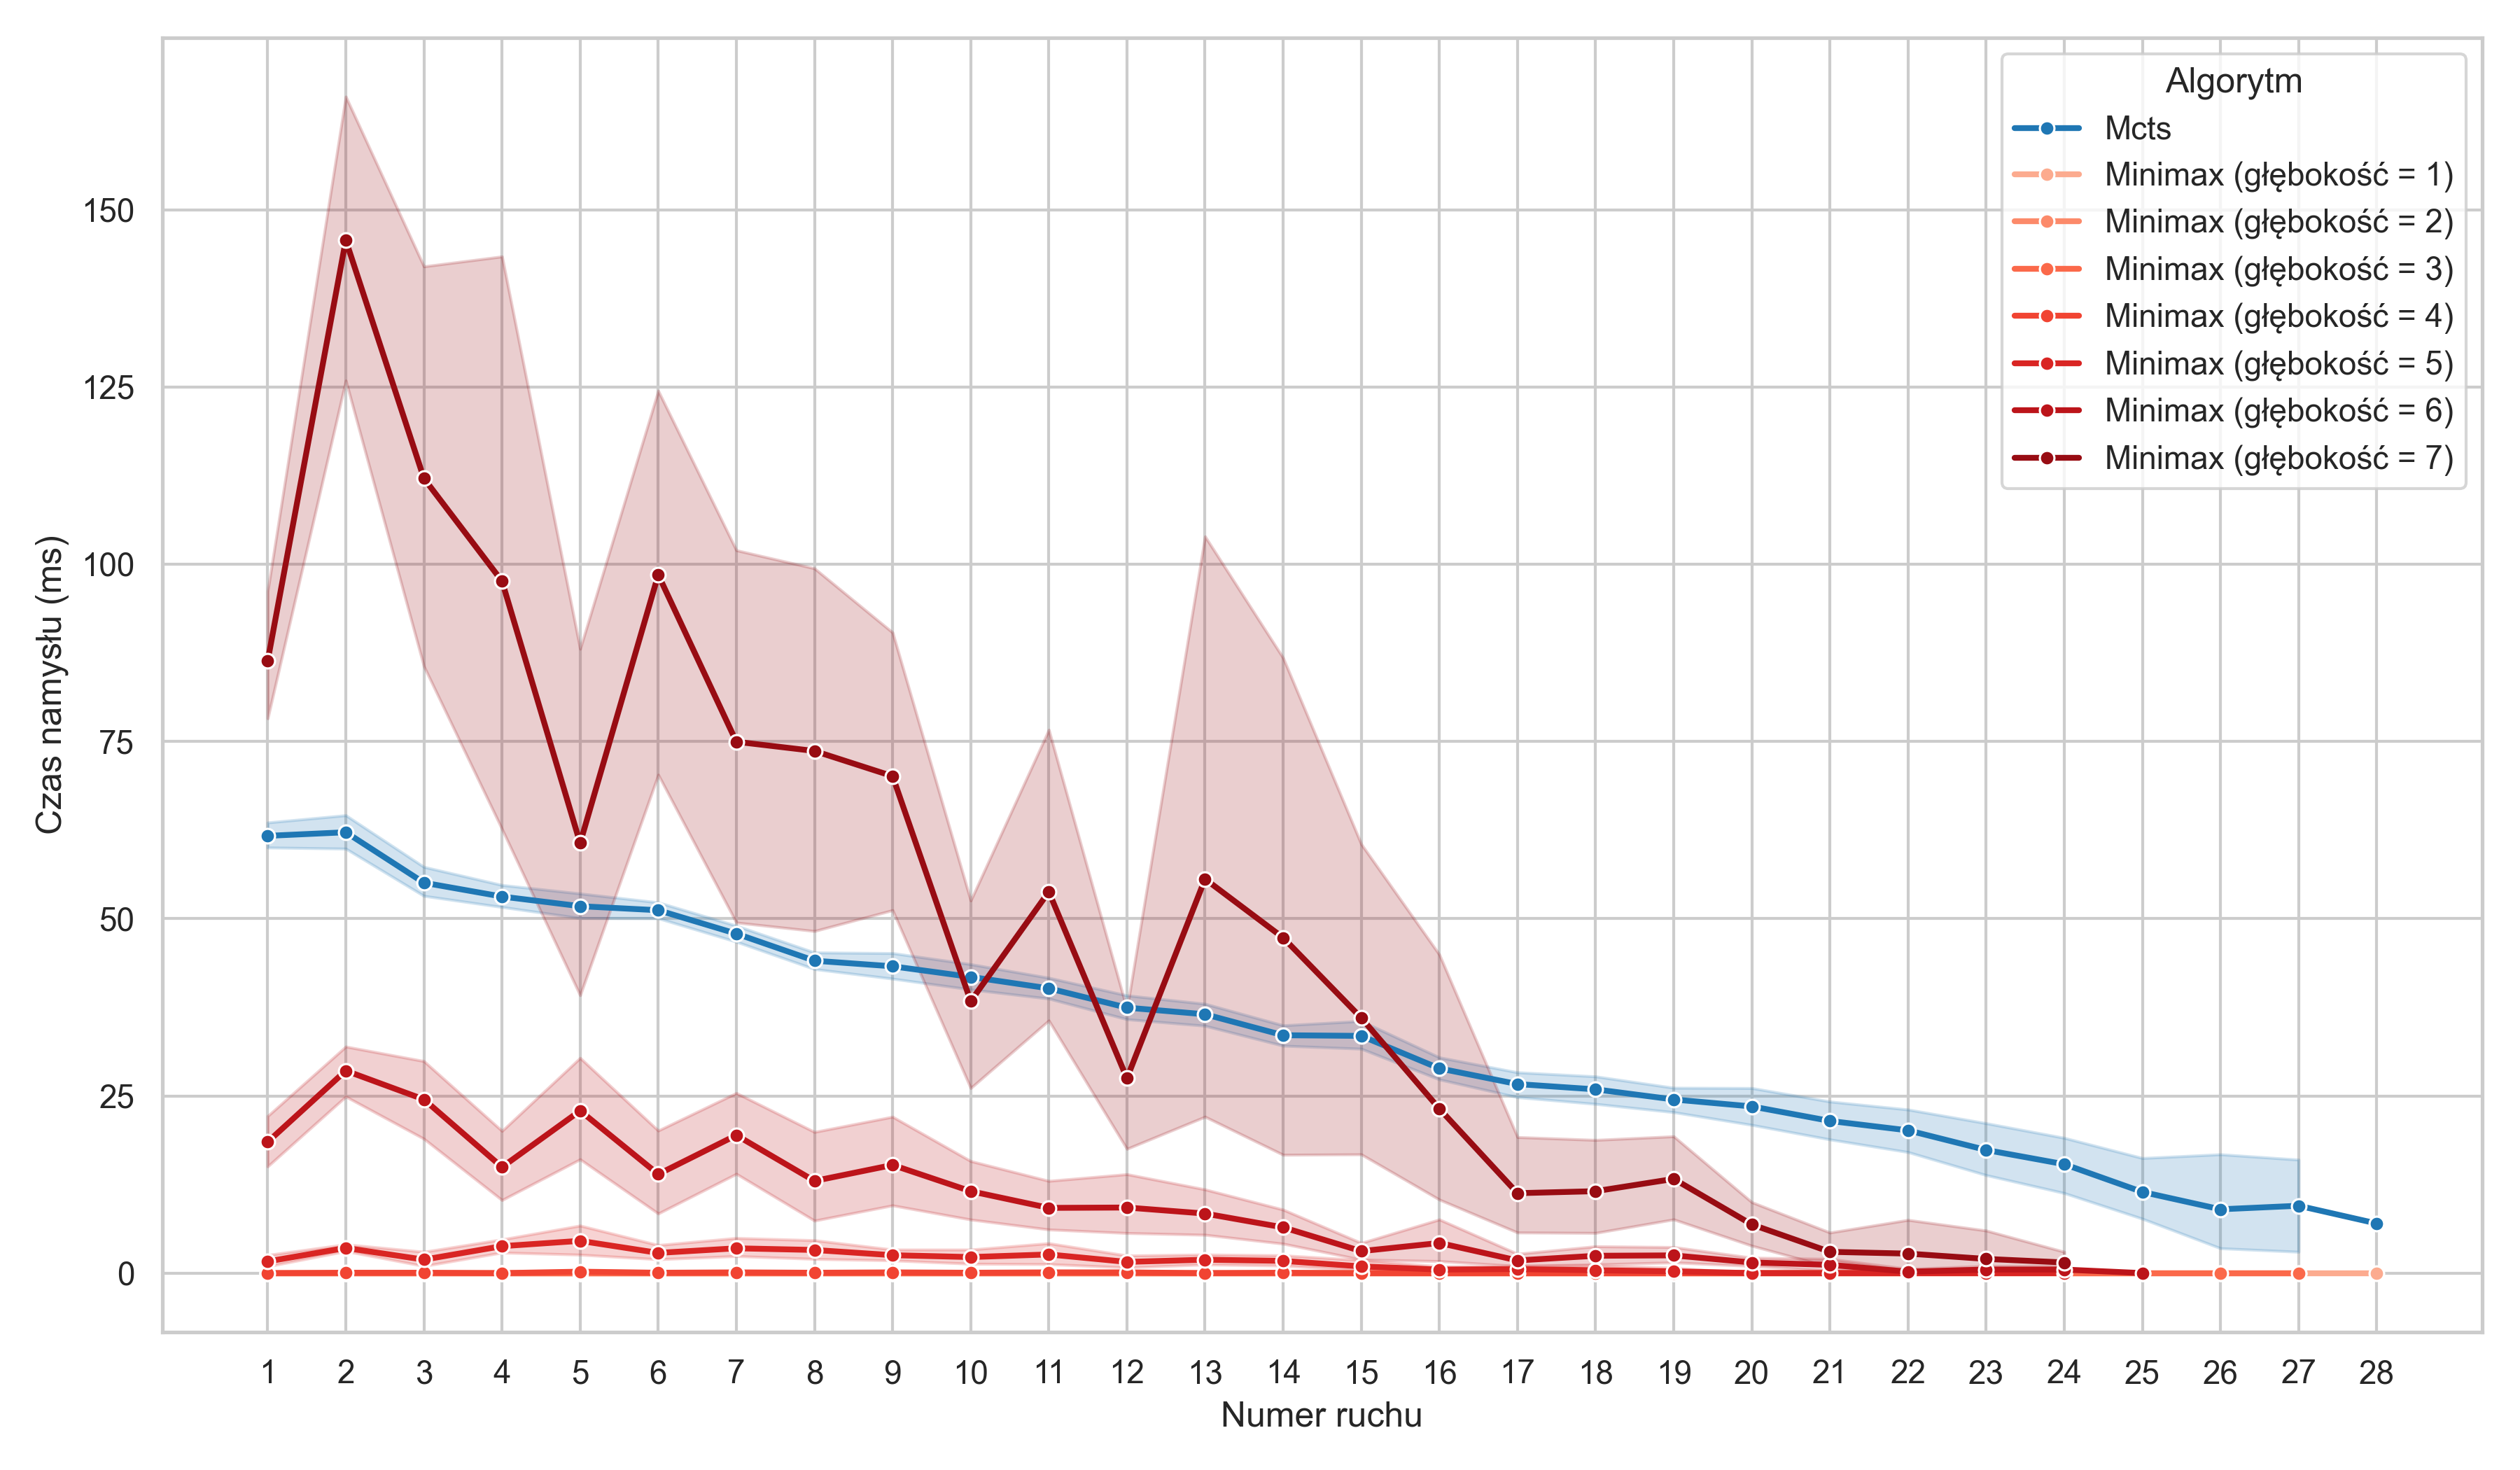
\includegraphics[width=\textwidth]{images/mcts_thinking_time.png}\\
        {\scriptsize MCTS}
    \end{minipage}%
    \hfill
    \begin{minipage}{0.30\textwidth}
        \centering
        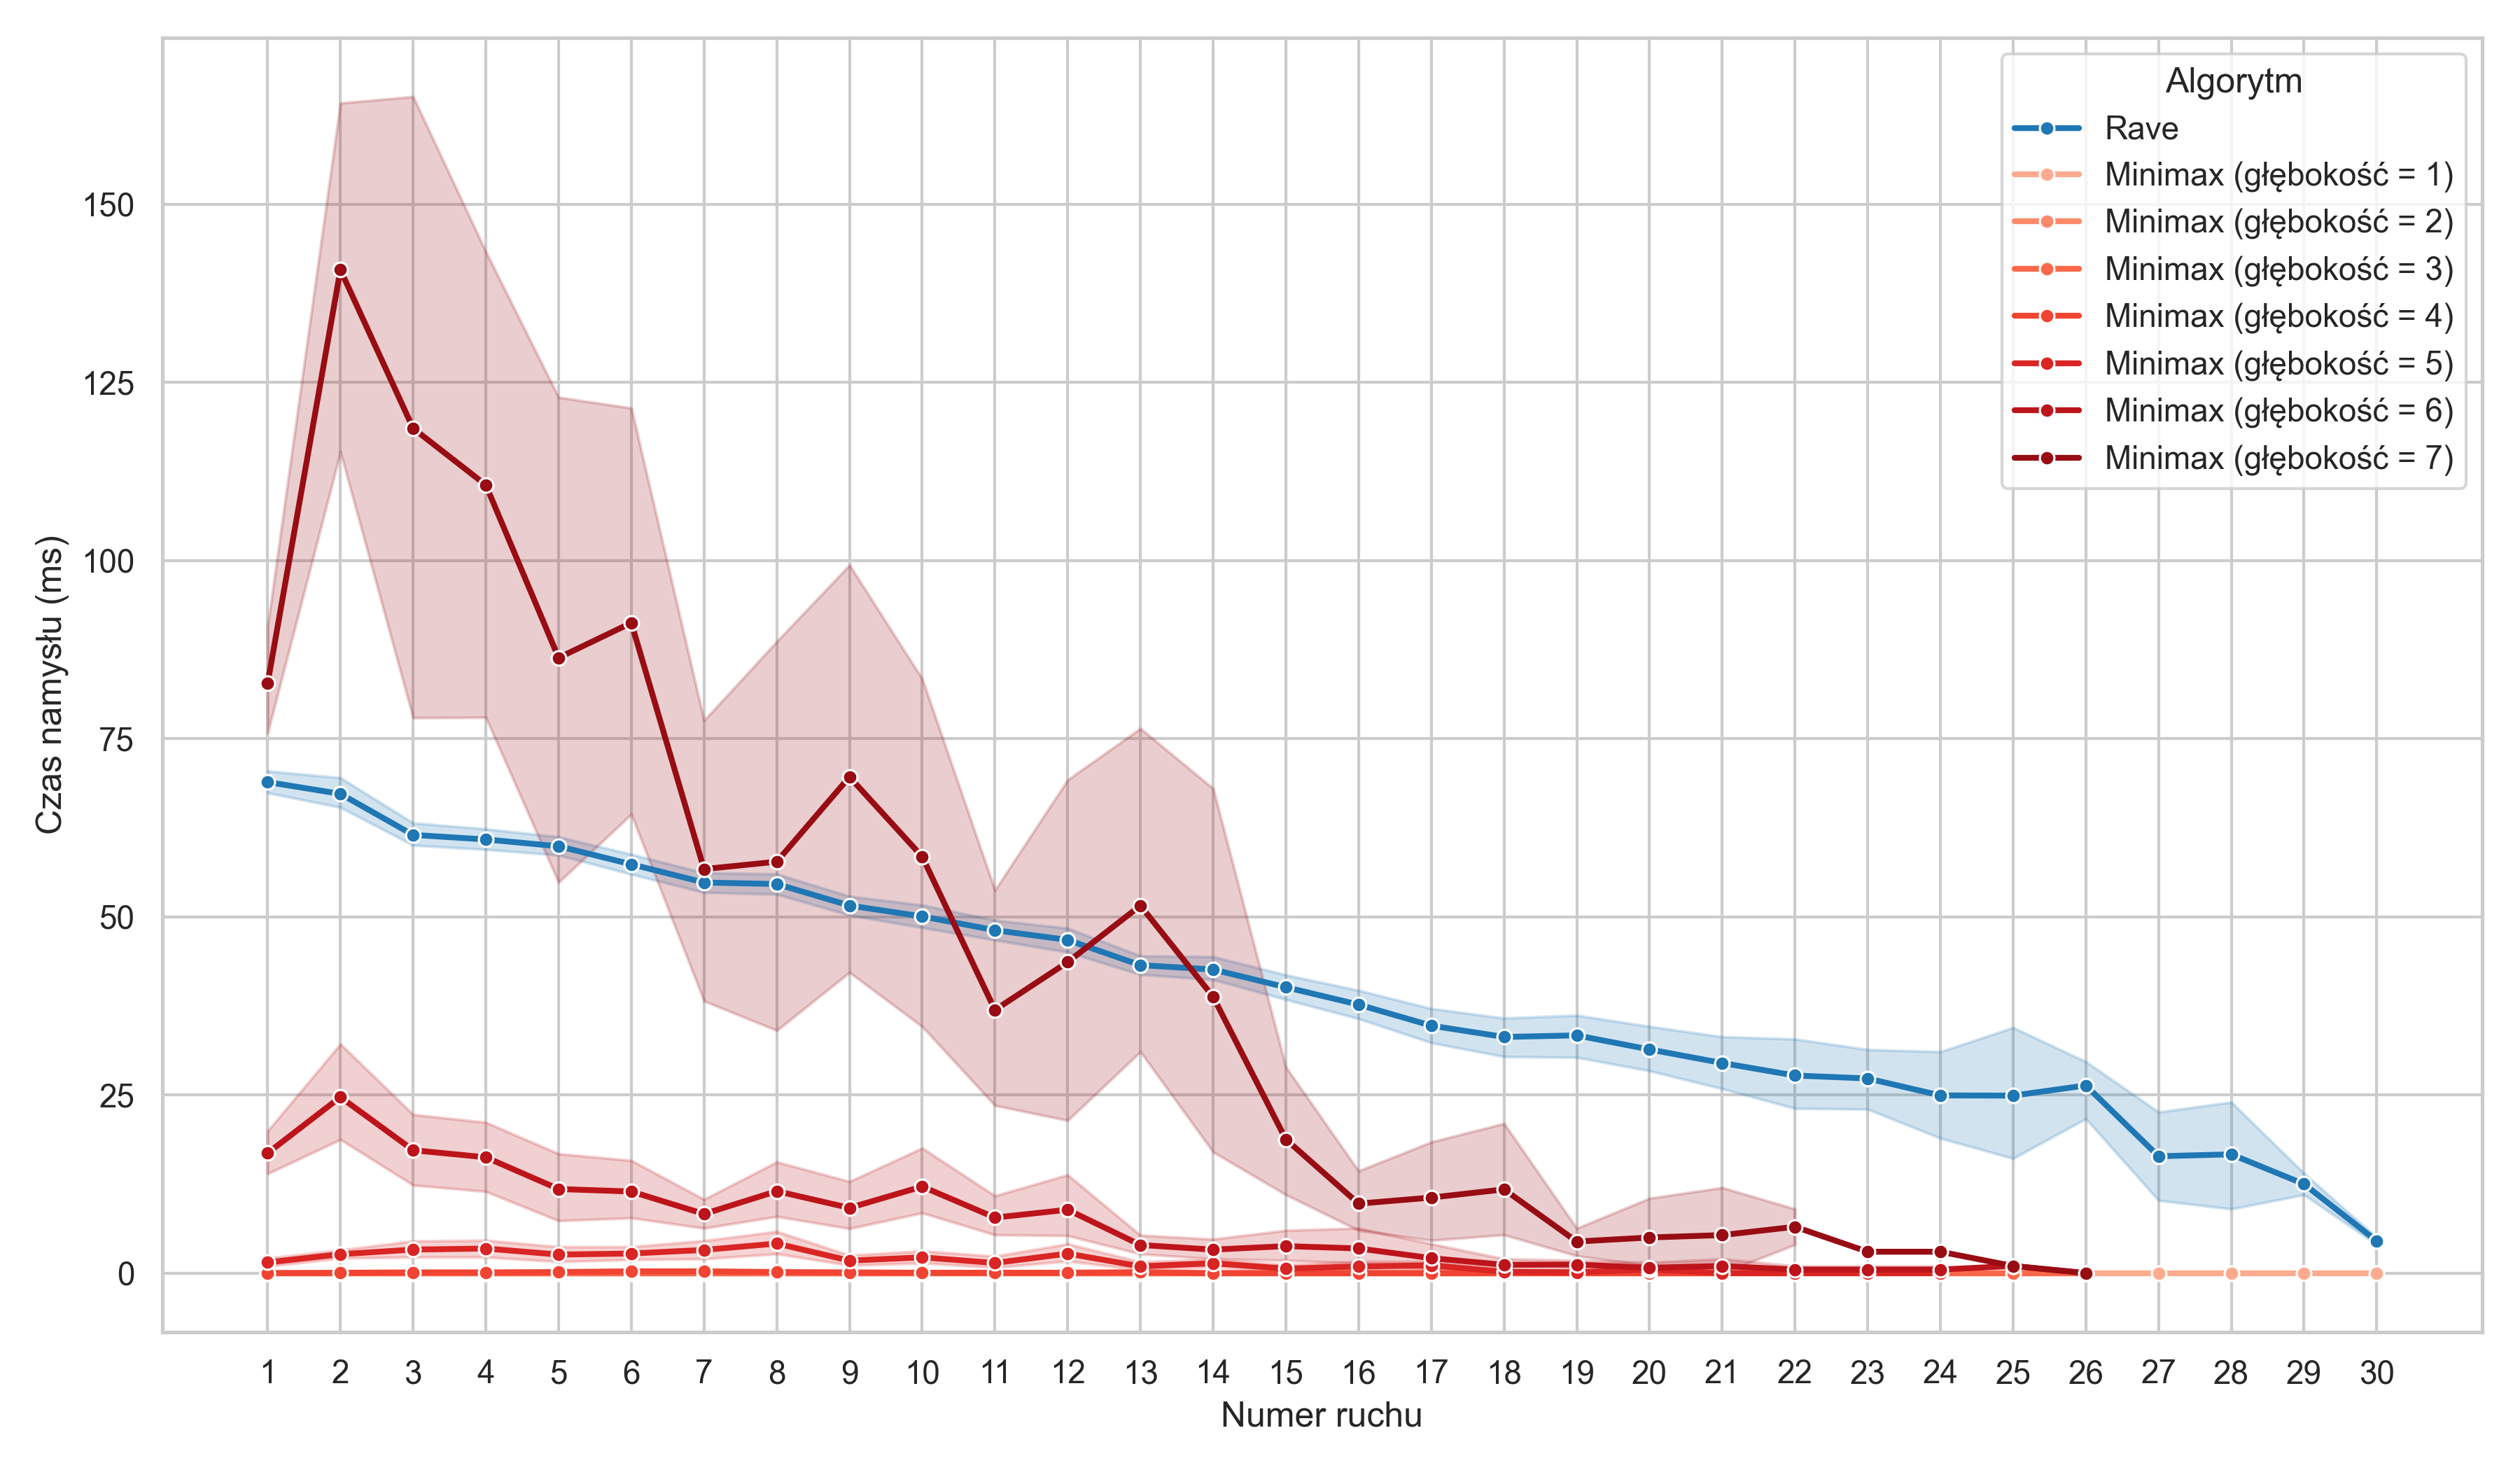
\includegraphics[width=\textwidth]{images/rave_thinking_time.png}\\
        {\scriptsize MCTS + RAVE}
    \end{minipage}%
    \hfill
    \begin{minipage}{0.30\textwidth}
        \centering
        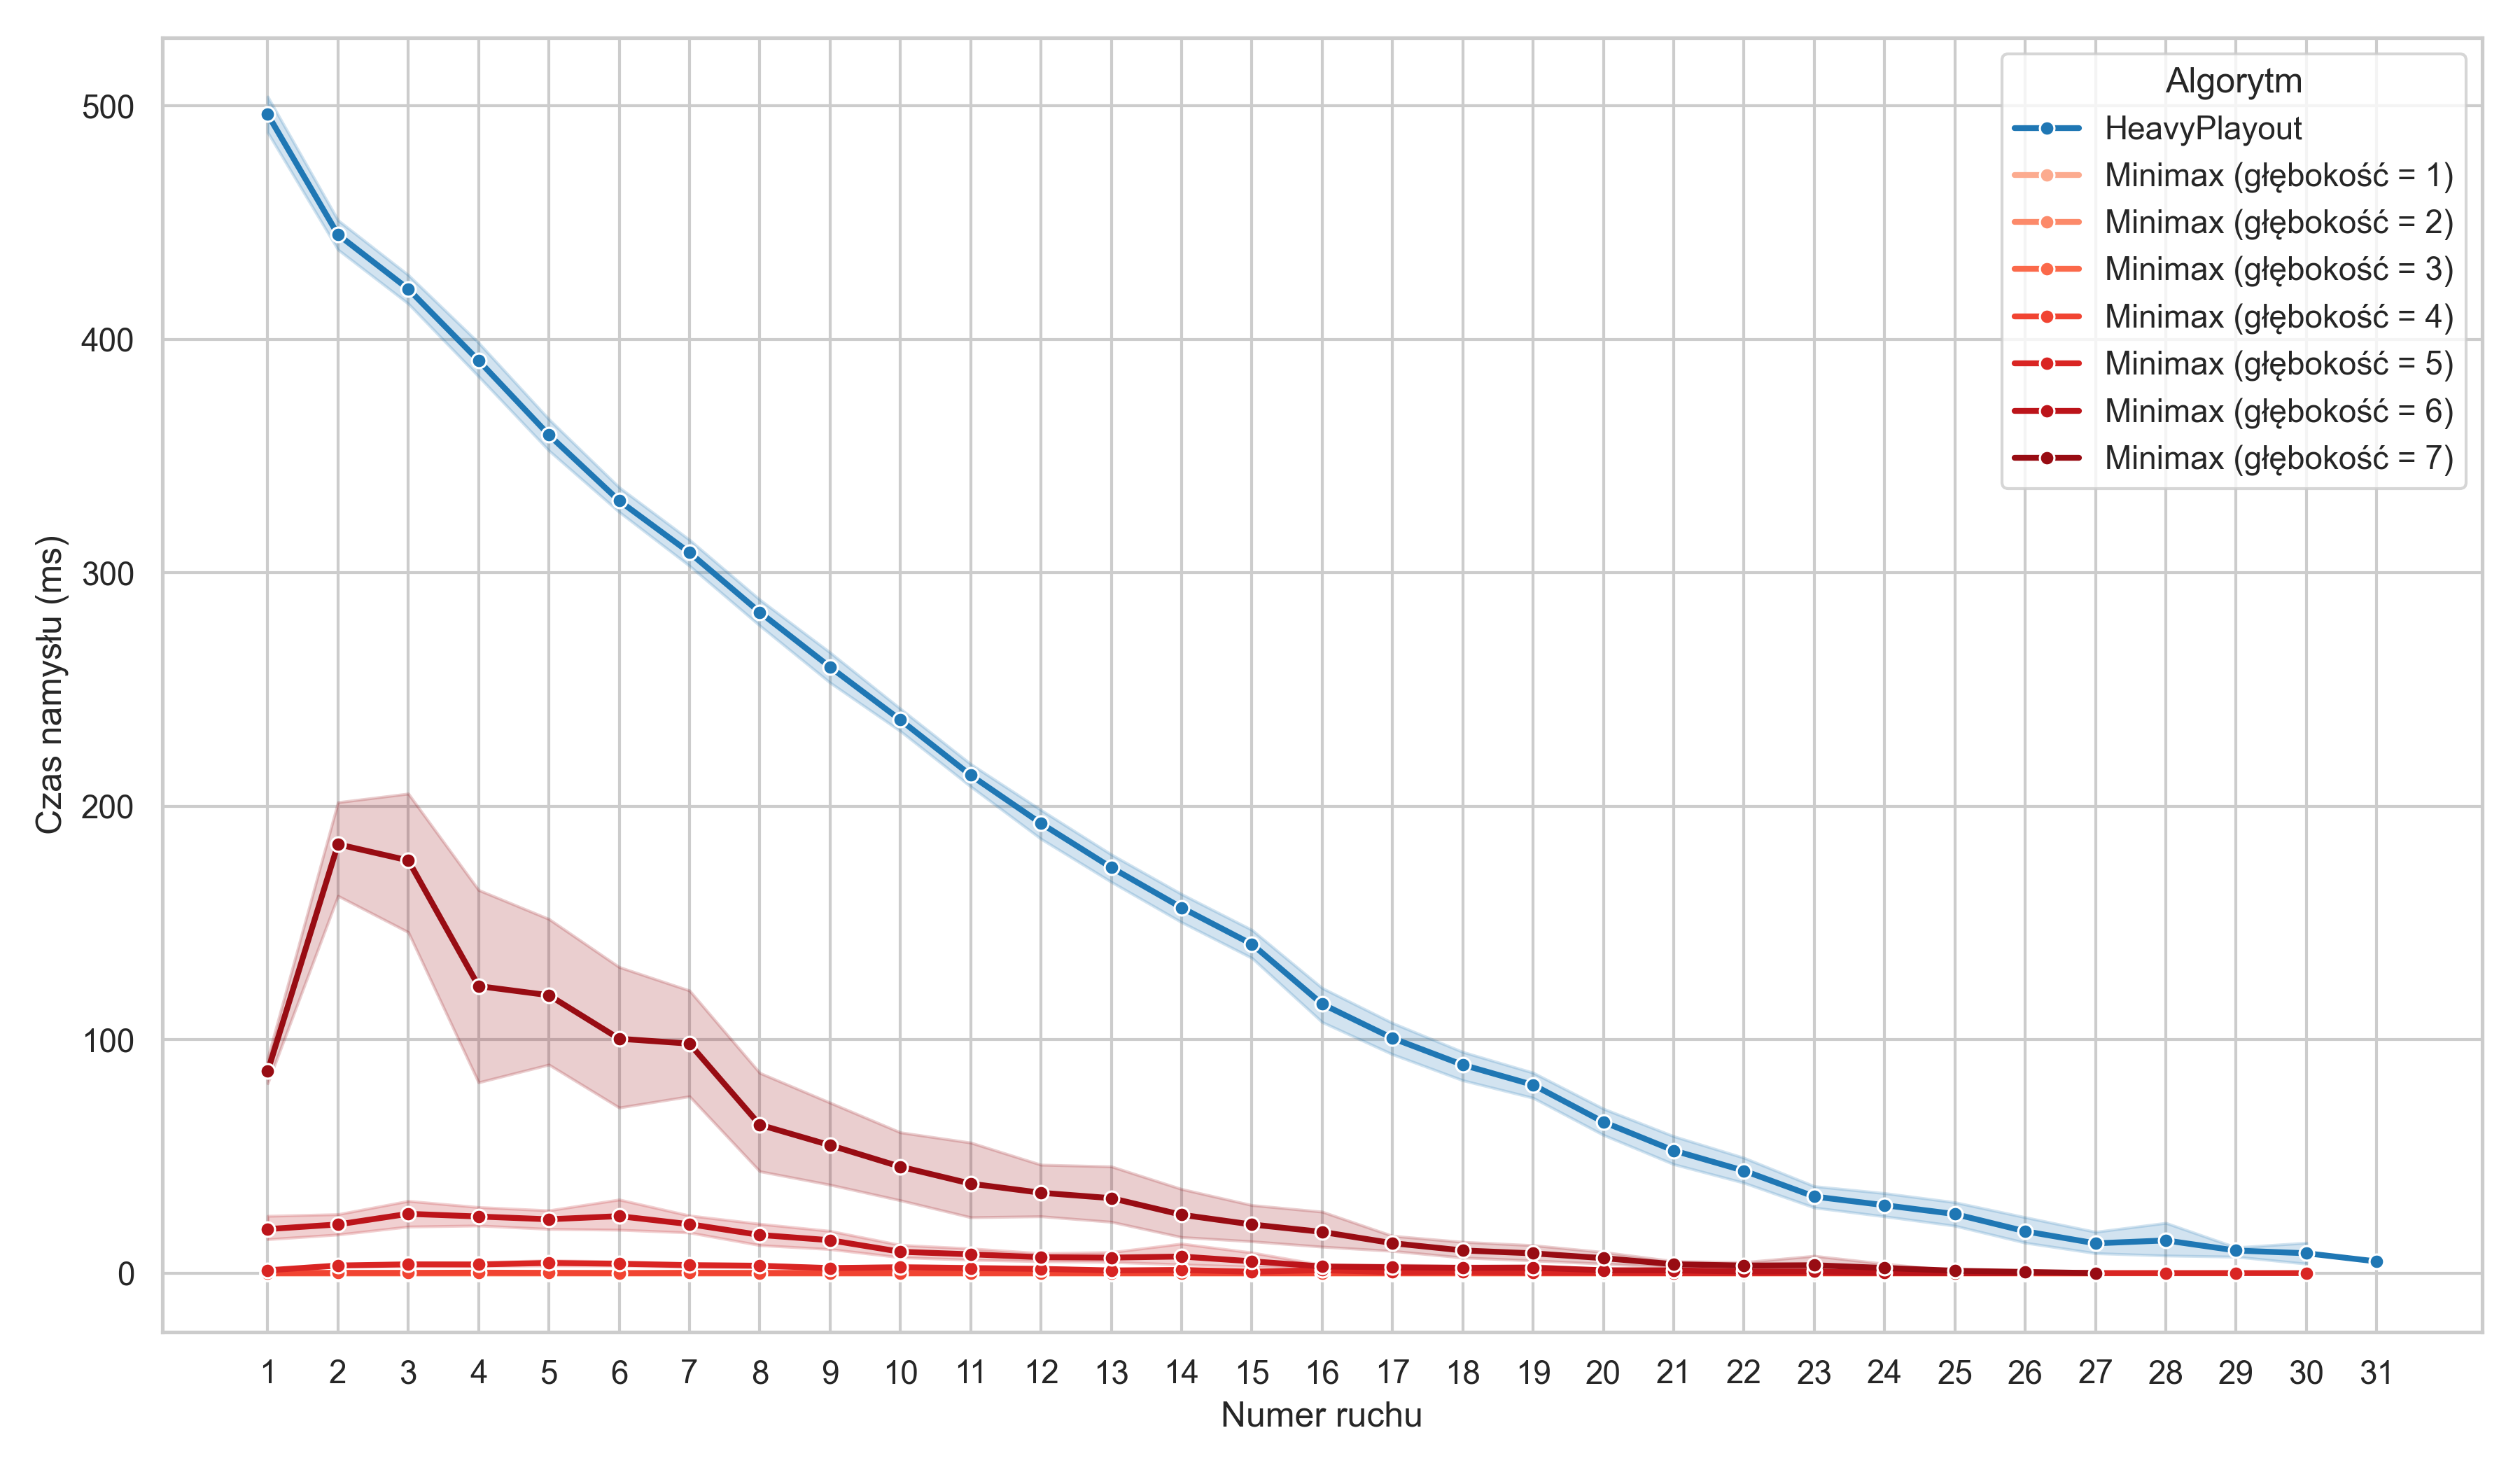
\includegraphics[width=\textwidth]{images/heavyplayouts_thinking_time.png}\\
        {\scriptsize MCTS + Heavy Playouts}
    \end{minipage}
    
    \vspace{0.7cm}
    
    Średni czas namysłu (w milisekundach) dla różnych wariantów algorytmu MCTS oraz ich przeciwników (agenta Minimax o rosnącej głębokości przeszukiwania).
\end{frame}

\begin{frame}{Wpływ rozmiaru planszy na asymetrię szans}
    \textbf{Metodologia}
    \begin{itemize}
        \item 3 warianty: MCTS, MCTS + RAVE, MCTS + Heavy Playouts
        \item Parametry planszy:
        \begin{itemize}
            \item stała szerokość $W = 8$
            \item zmienna wysokość $H \in \{5,6,7,8,9,10,11\}$
        \end{itemize}
        \item Budżet obliczeniowy: $I = 2000 \cdot H$
        \item Identyczni agenci po obu stronach planszy
        \item 50 partii dla każdego rozmiaru planszy
    \end{itemize}
    \textbf{Metryki:}
    \begin{itemize}
        \item Współczynnik zwycięstw dla białych
    \end{itemize}
\end{frame}

\begin{frame}{Średni czas namysłu}
    \centering
    \begin{minipage}{0.30\textwidth}
        \centering
        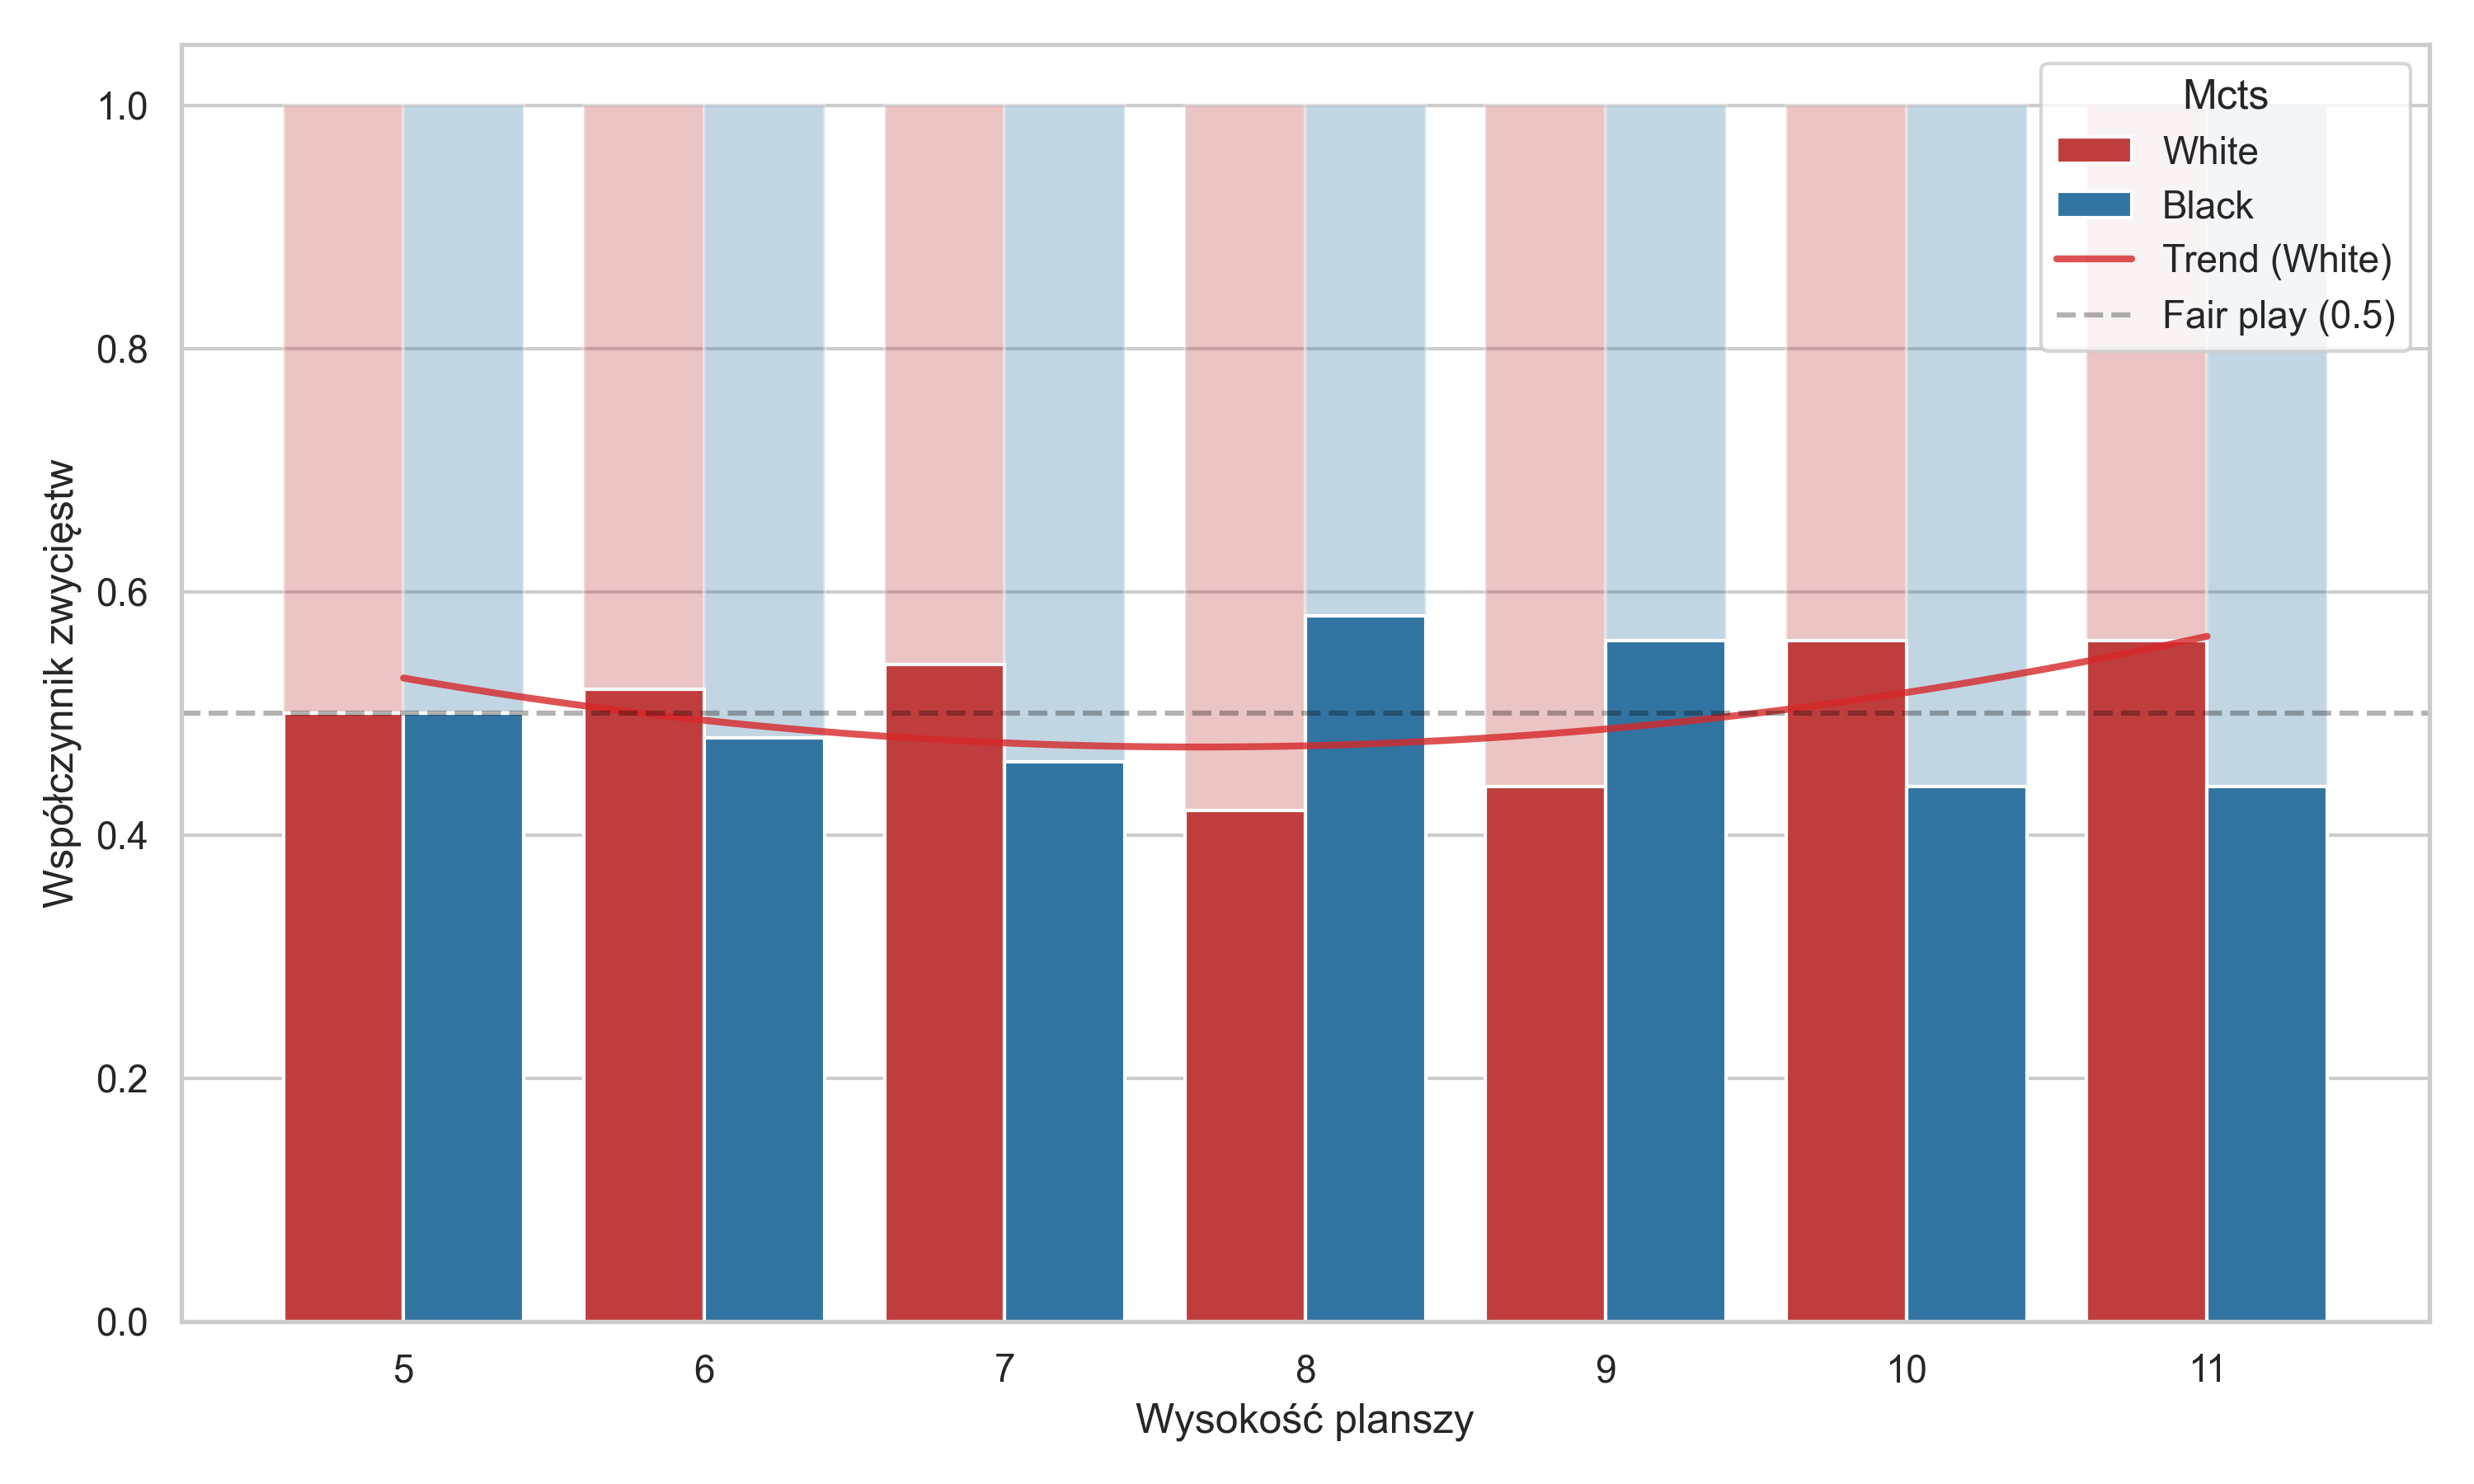
\includegraphics[width=\textwidth]{images/mcts_board_size_win_rate.png}\\
        {\scriptsize MCTS}
    \end{minipage}%
    \hfill
    \begin{minipage}{0.30\textwidth}
        \centering
        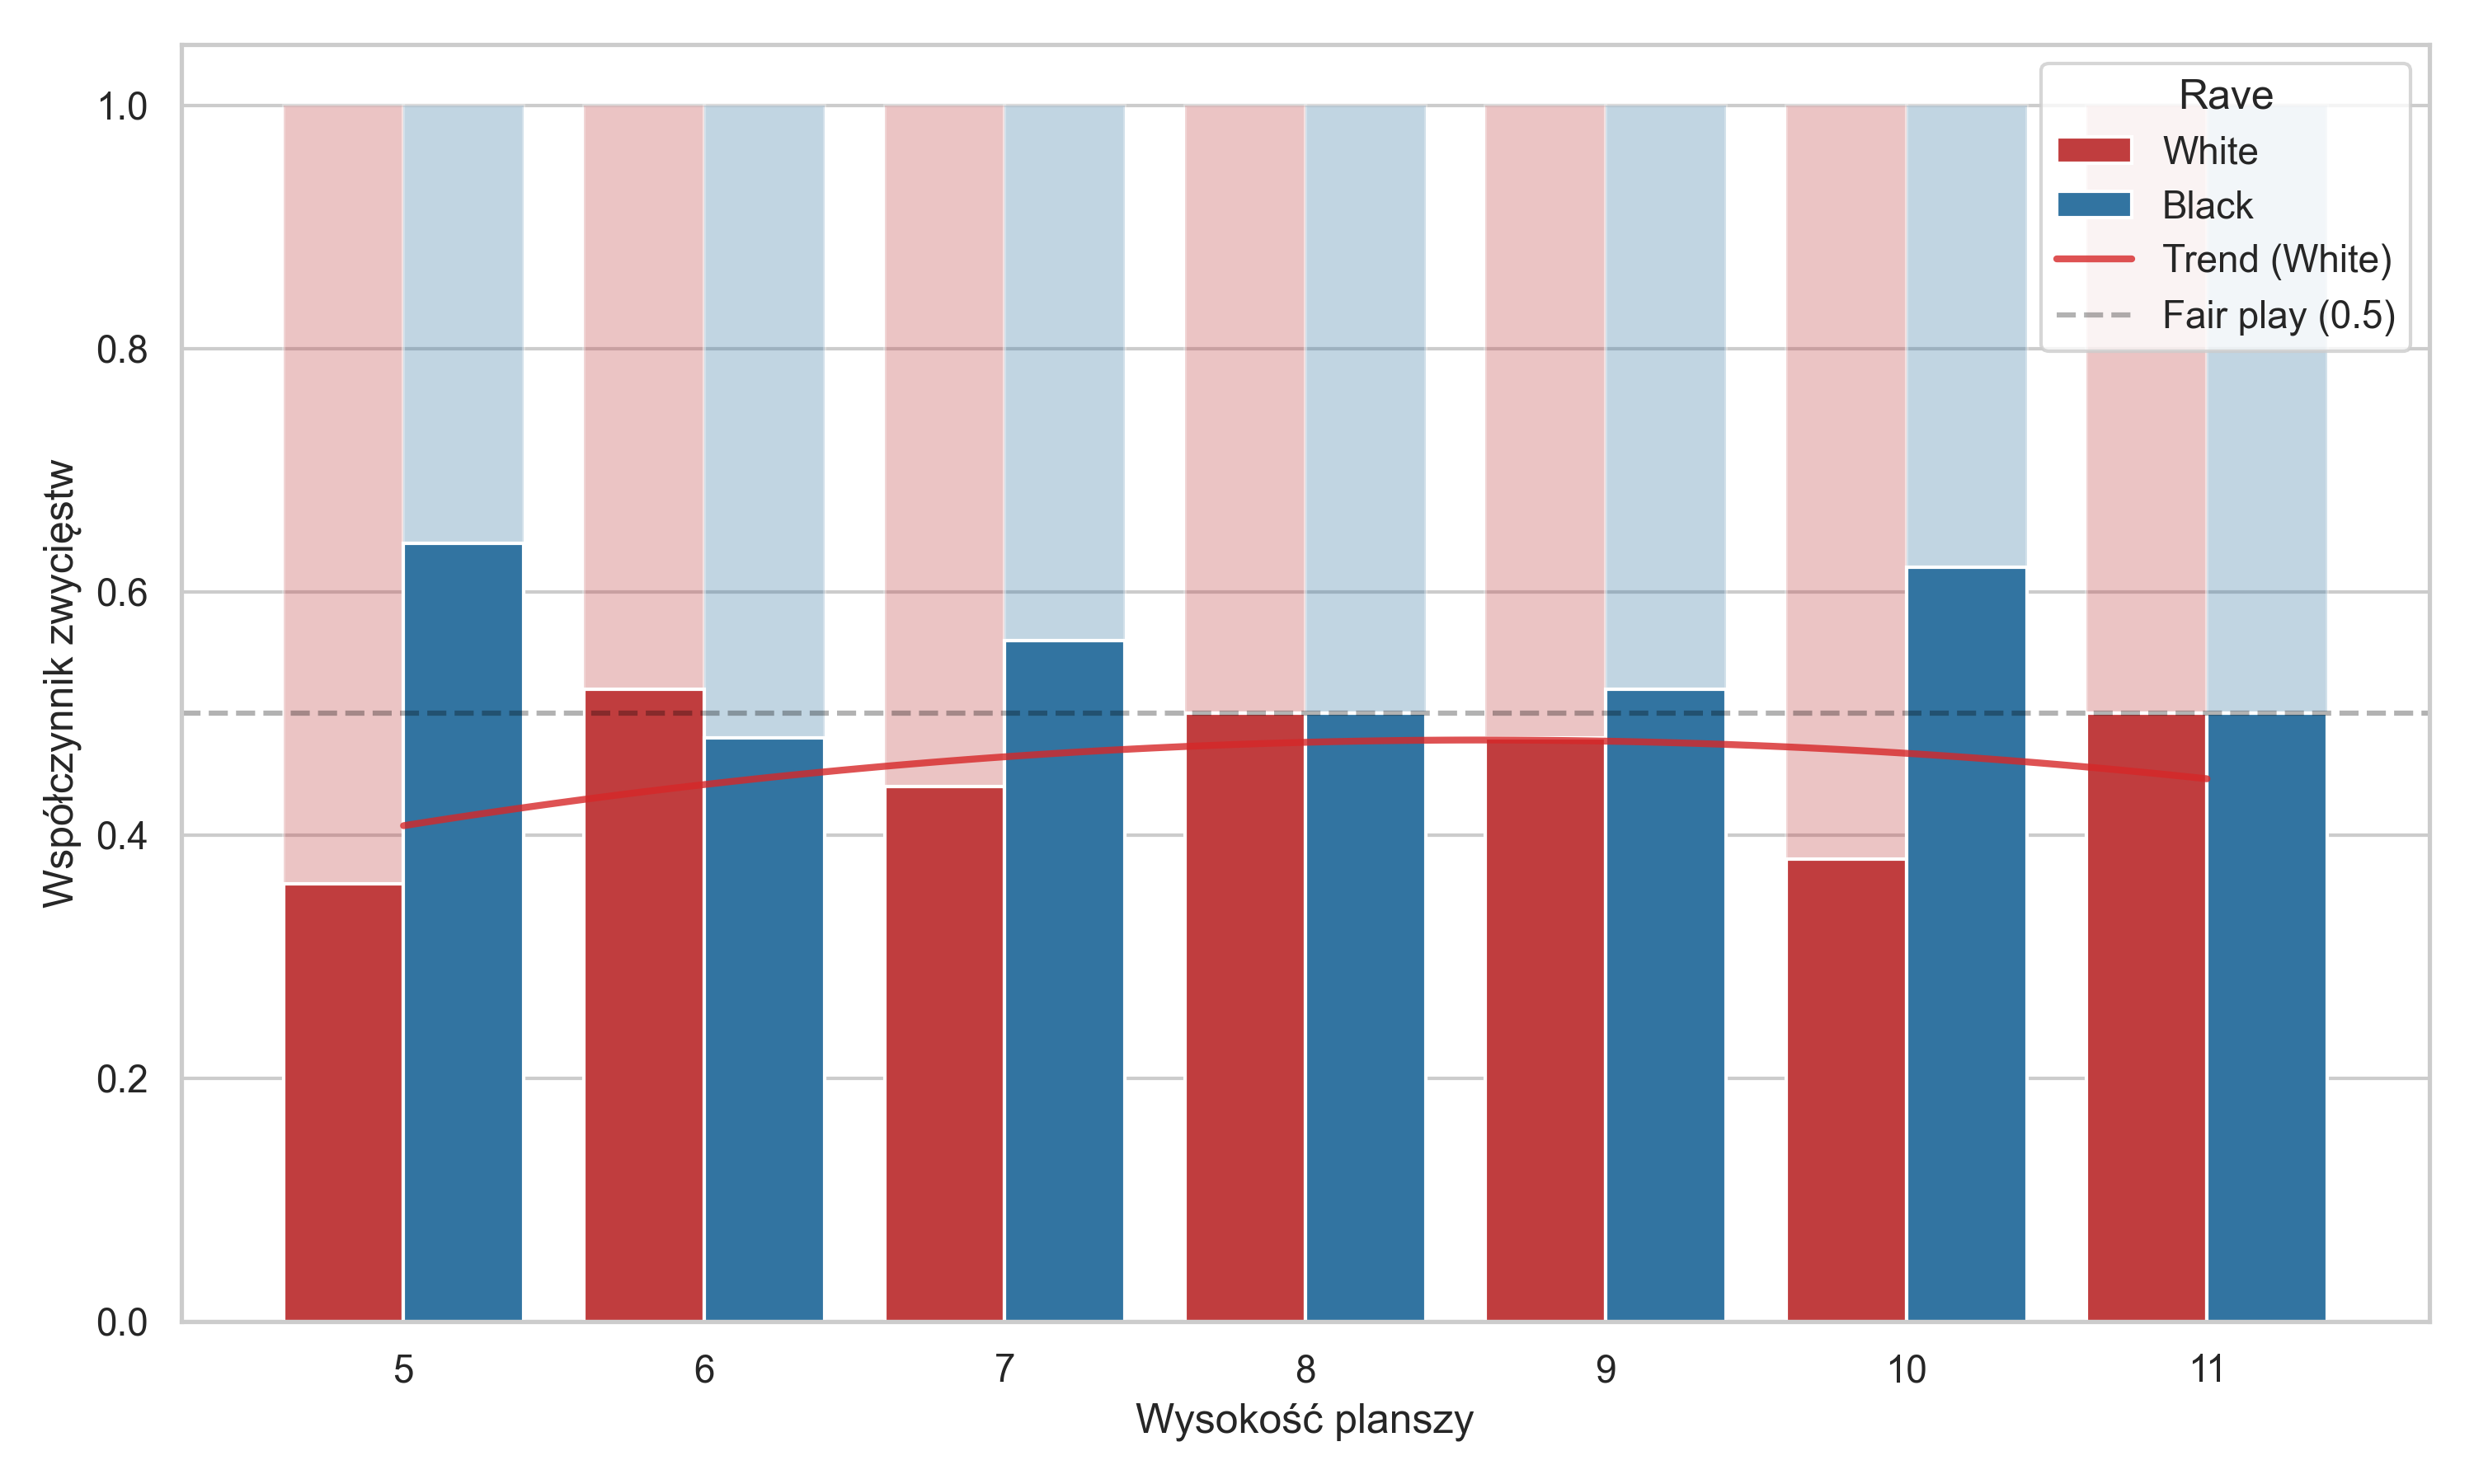
\includegraphics[width=\textwidth]{images/rave_board_size_win_rate.png}\\
        {\scriptsize MCTS + RAVE}
    \end{minipage}%
    \hfill
    \begin{minipage}{0.30\textwidth}
        \centering
        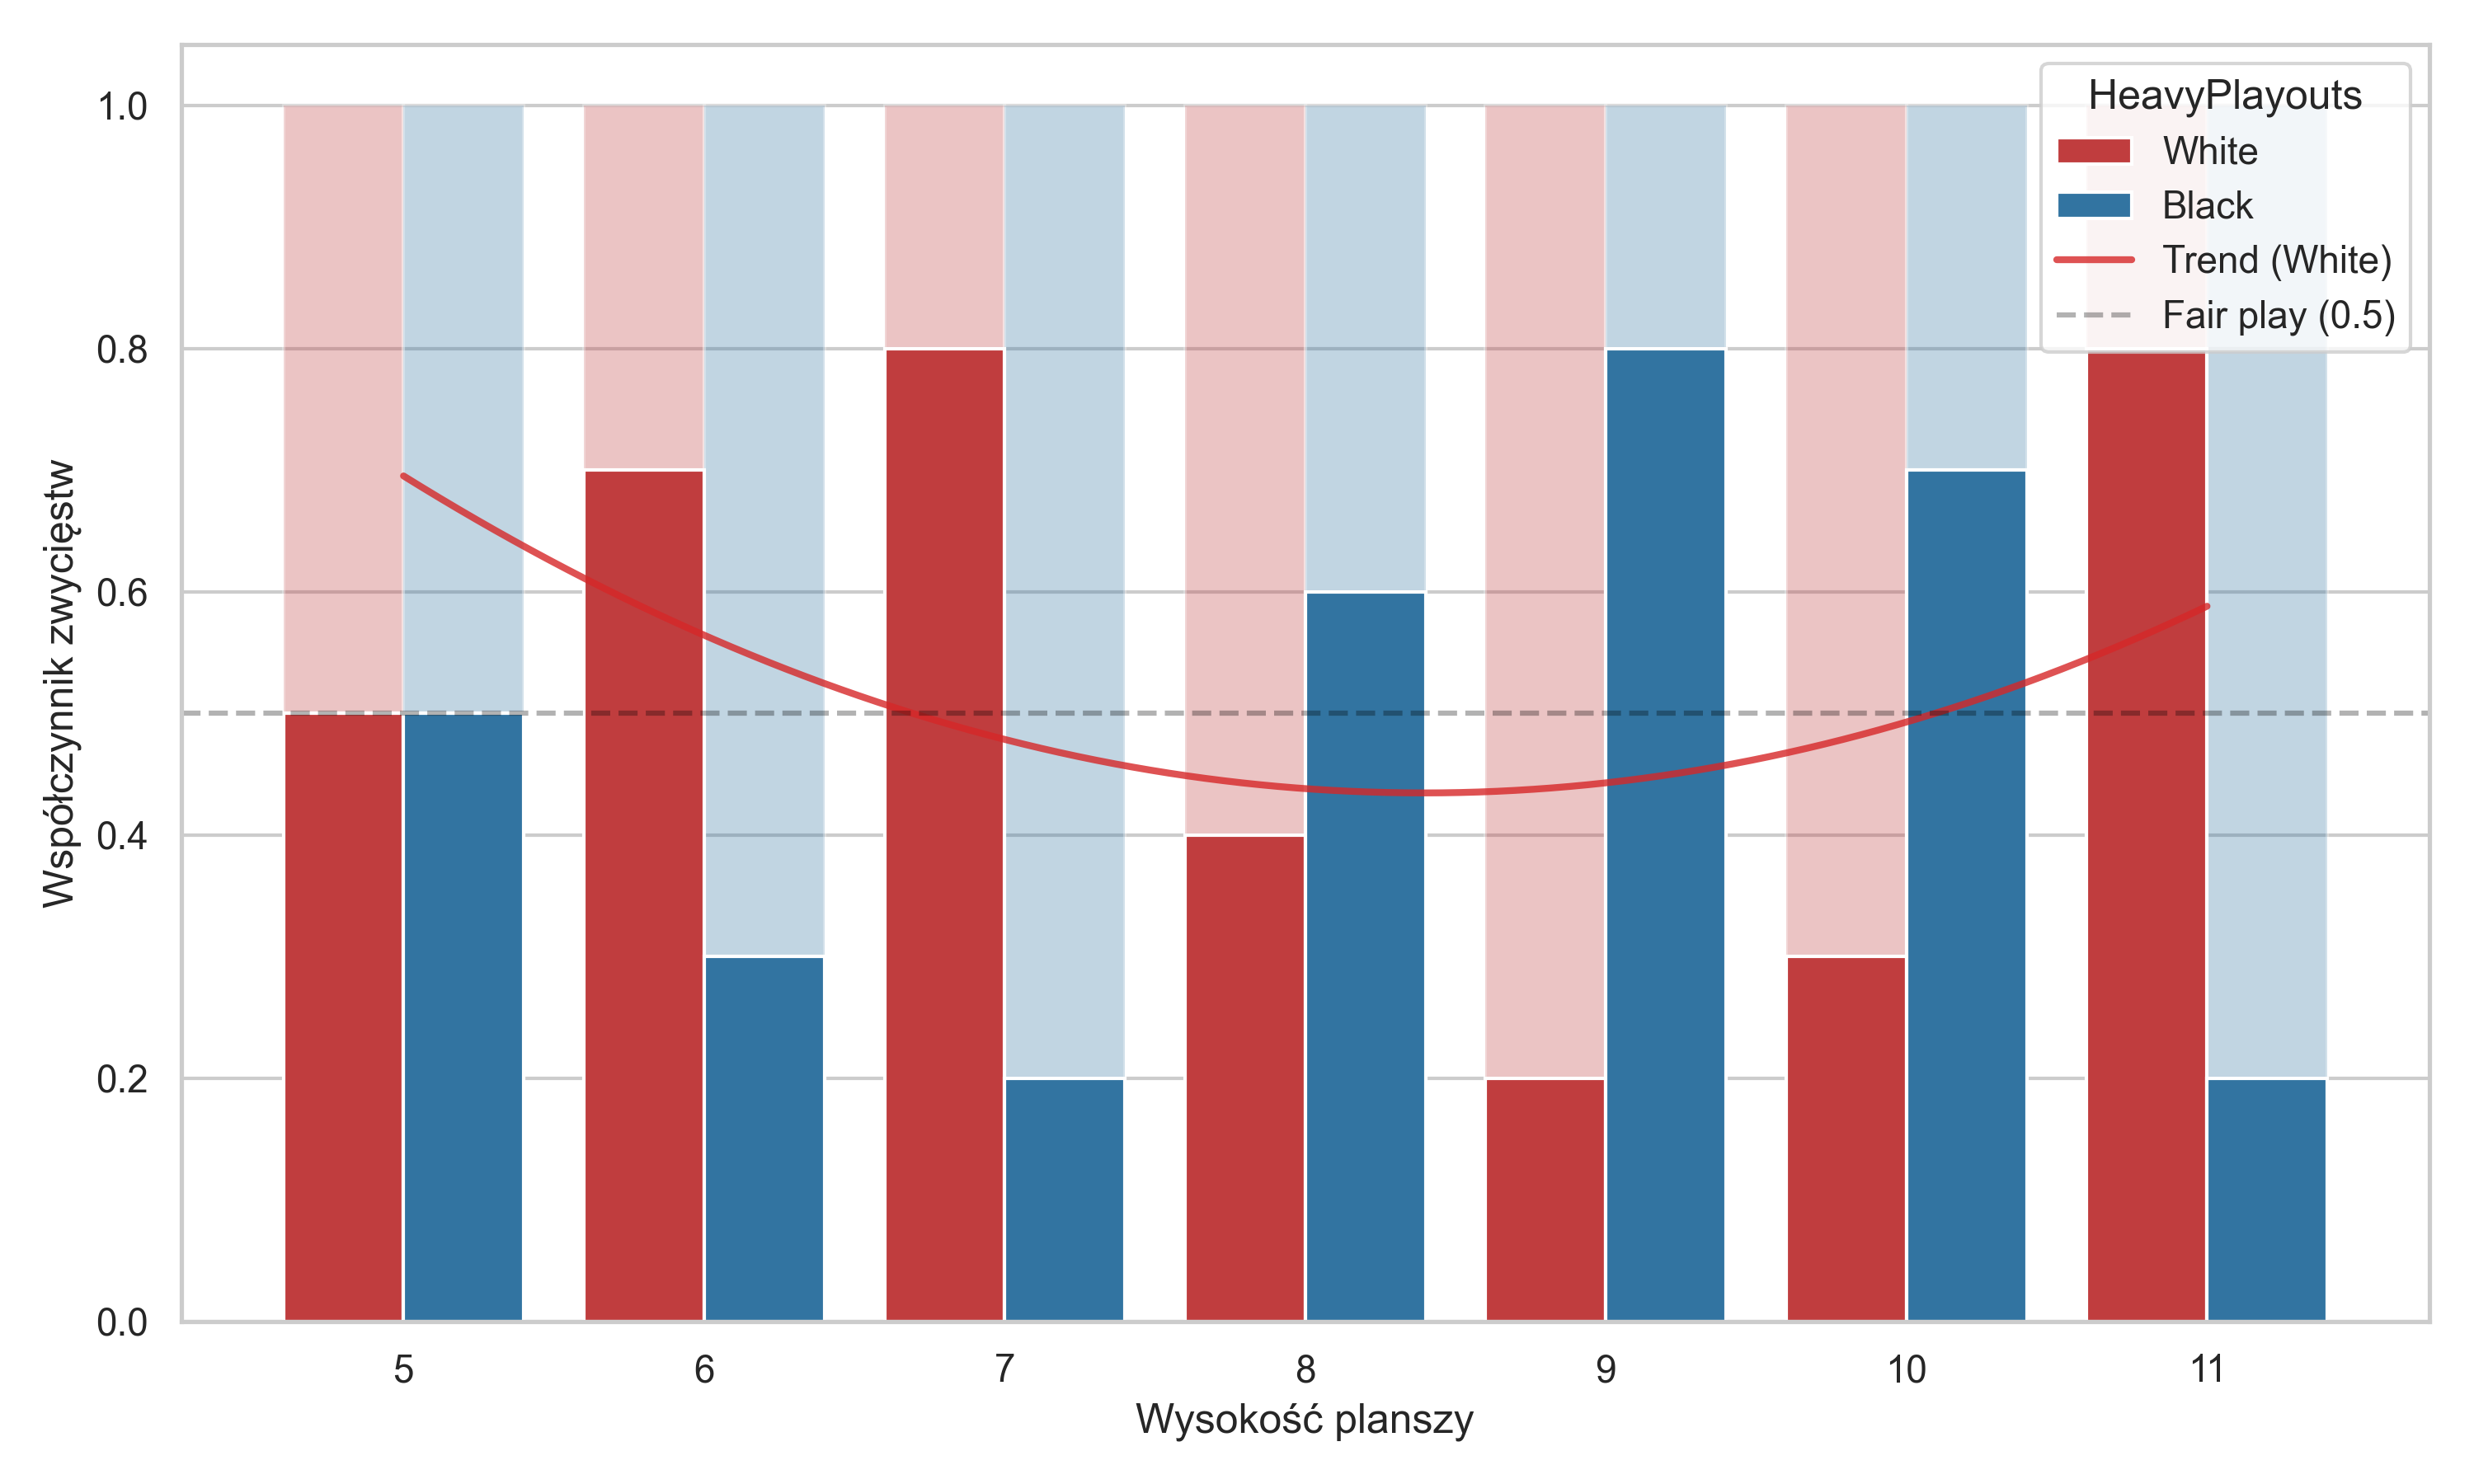
\includegraphics[width=\textwidth]{images/heavyplayouts_board_size_win_rate.png}\\
        {\scriptsize MCTS + Heavy Playouts}
    \end{minipage}
    
    \vspace{0.7cm}
    
    Odsetek zwycięstw gracza rozpoczynającego (Białe) w starciach symetrycznych w zależności od wysokości planszy ($H$) przy stałej szerokości $W=8$.
\end{frame}

\begin{frame}{Wpływ modyfikacji RAVE na MCTS -- metodologia}
    \begin{columns}[T]
    \begin{column}{0.52\textwidth}
        \structure{\textbf{Cel eksperymentu}}
        \vspace{0.1cm}
        \begin{itemize}
            \item Bezpośrednie porównanie MCTS + RAVE z klasycznym MCTS.
            \item Kryterium sukcesu: ponad 55\% zwycięstw agenta RAVE.
            \item Stały budżet: 10~000 iteracji na ruch dla obu agentów.
        \end{itemize}
    \end{column}

    \begin{column}{0.43\textwidth}
        \structure{\textbf{Dobór parametru $k$}}
        \vspace{0.1cm}
        \begin{itemize}
            \item Testowano wpływ parametru $k$ na wagę AMAF.
            \item Wybrano $k=100$, bo dawało lepsze wyniki niż domyślne $k=1000$.
            \item Mniejsze $k$ szybciej przełącza algorytm z RAVE na klasyczne statystyki UCT.
        \end{itemize}
    \end{column}
    \end{columns}

    \vspace{0.35cm}

    \structure{\textbf{Zakres testów}}
    \begin{itemize}
        \item Plansze: $6 \times 8$, $7 \times 7$, $8 \times 6$, $8 \times 8$.
        \item 50 partii na każdy rozmiar planszy: 25 jako białe i 25 jako czarne.
        \item Łącznie 200 partii.
    \end{itemize}
\end{frame}

\begin{frame}{Wpływ modyfikacji RAVE na MCTS -- wyniki}
    \centering
    \begin{minipage}{0.48\textwidth}
        \centering
        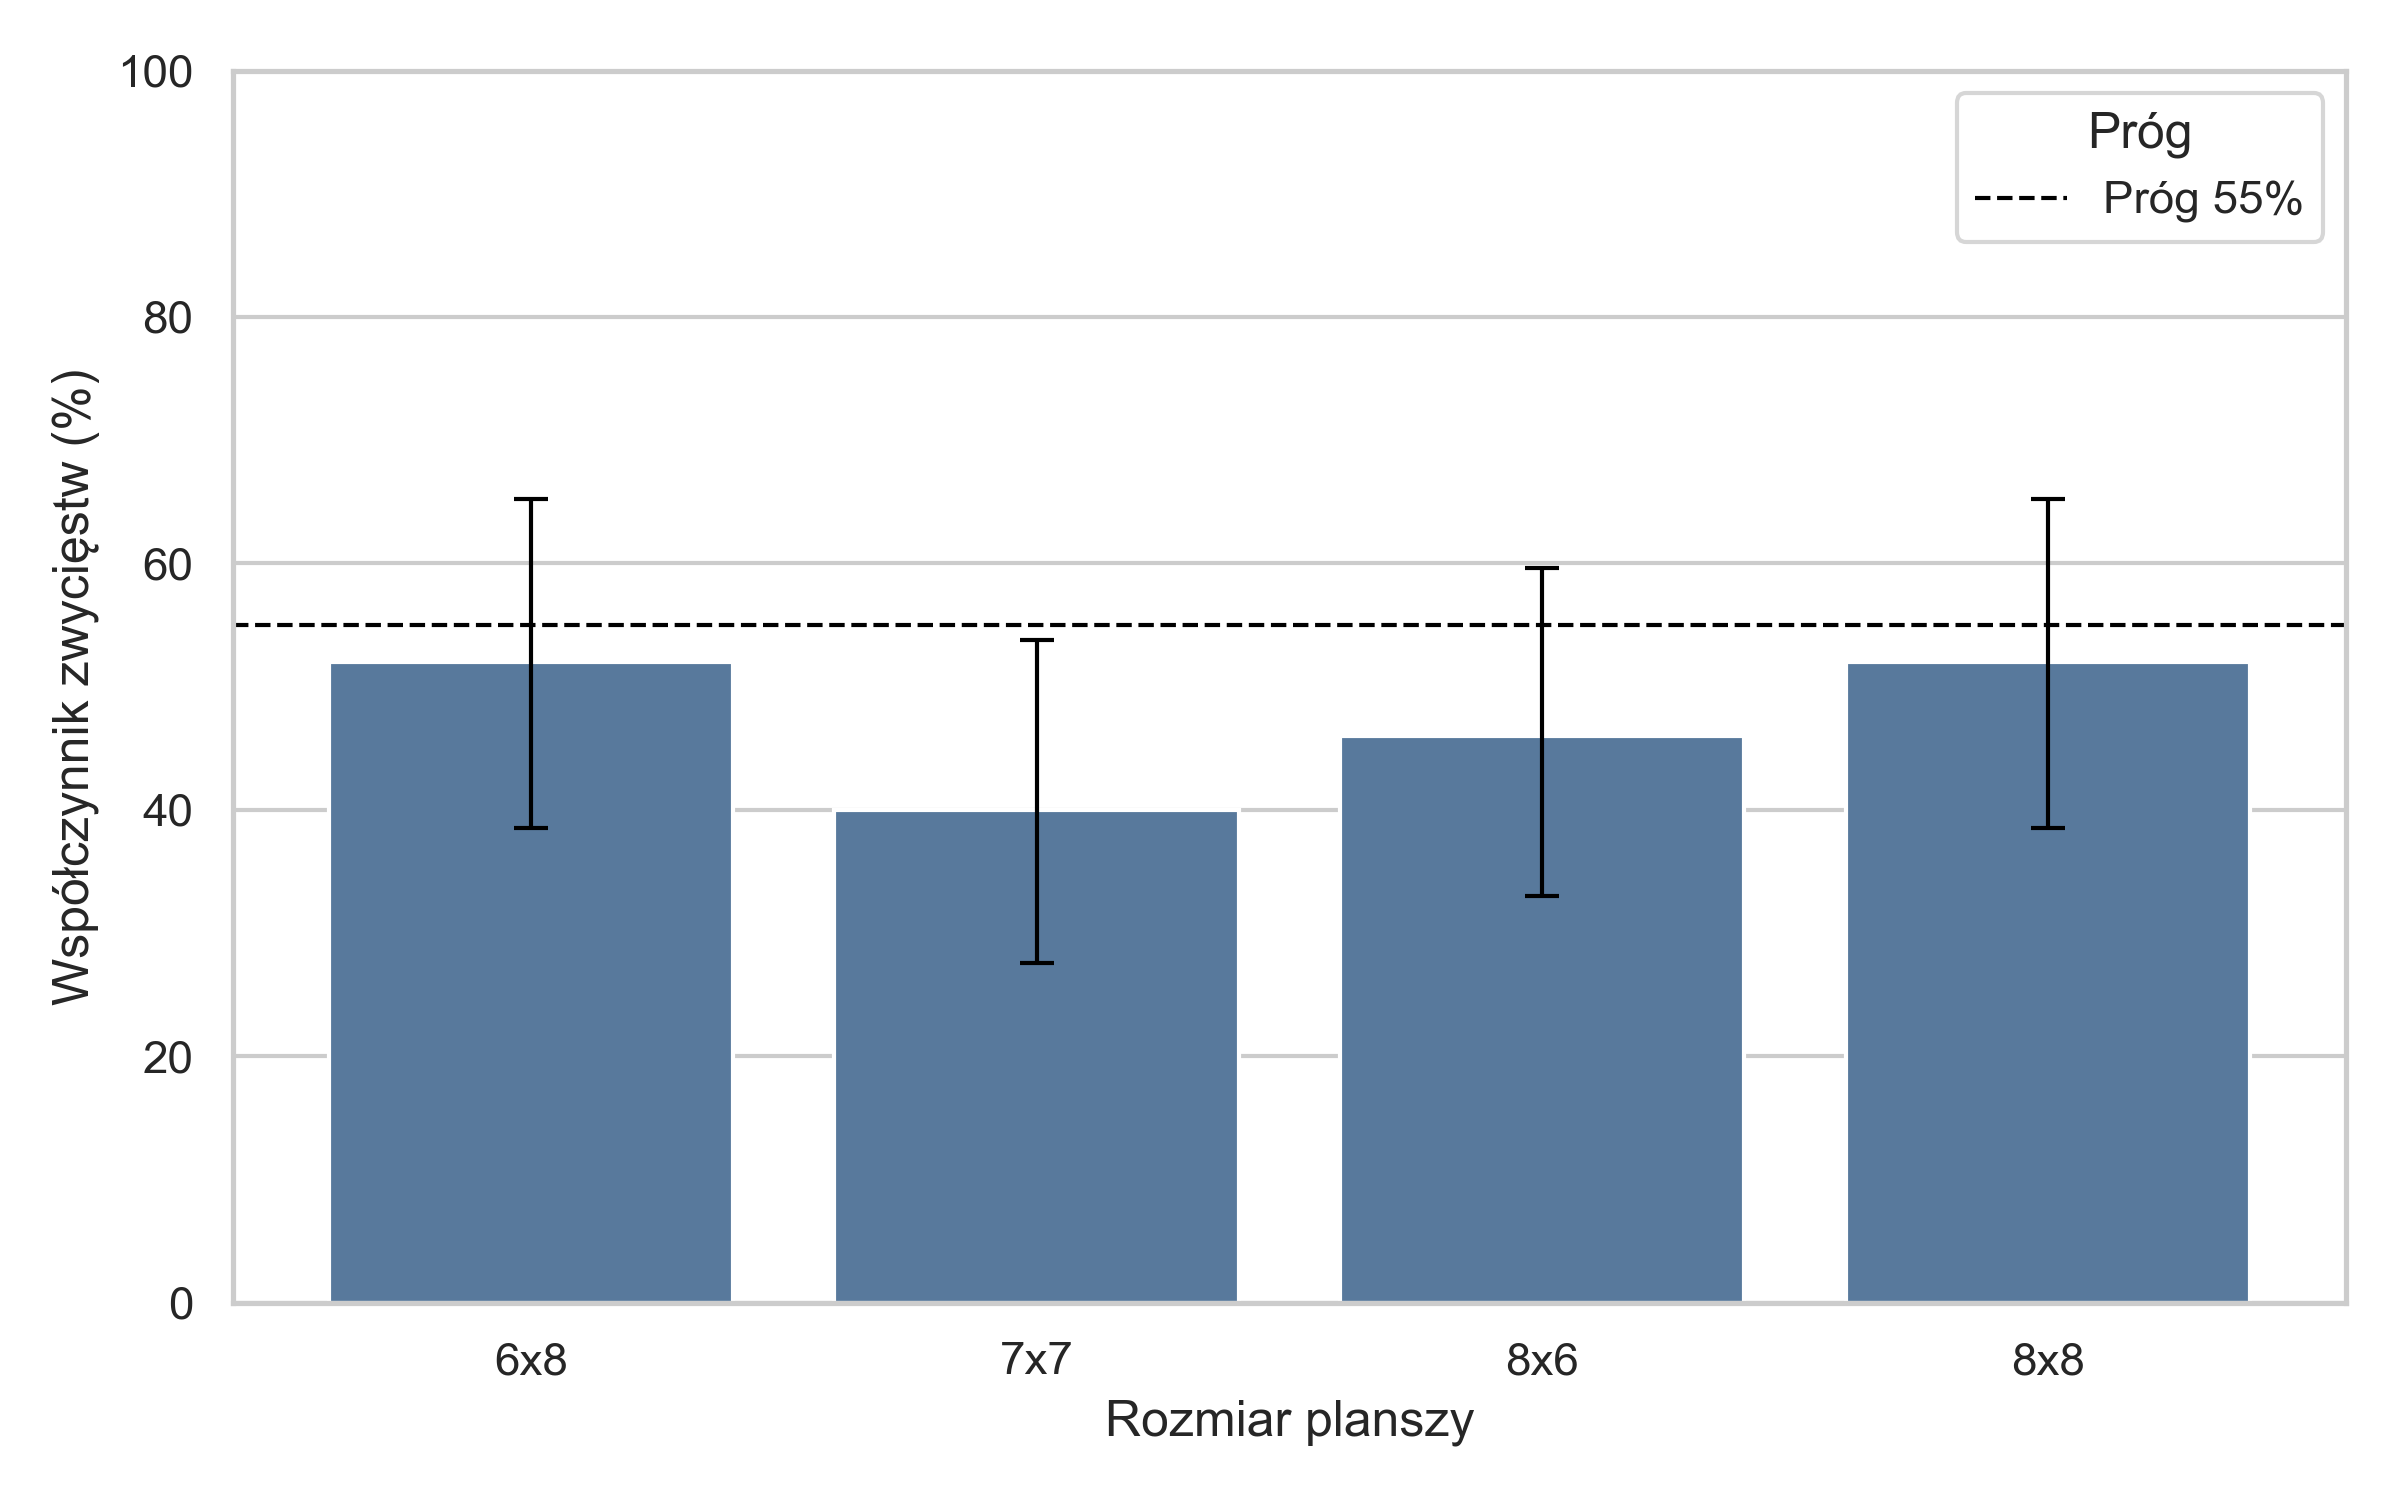
\includegraphics[width=0.92\textwidth]{images/h1_rave_win_rate_by_board.png}

        \vspace{0.05cm}
        {\scriptsize Wyniki według rozmiaru planszy}
    \end{minipage}
    \hfill
    \begin{minipage}{0.48\textwidth}
        \centering
        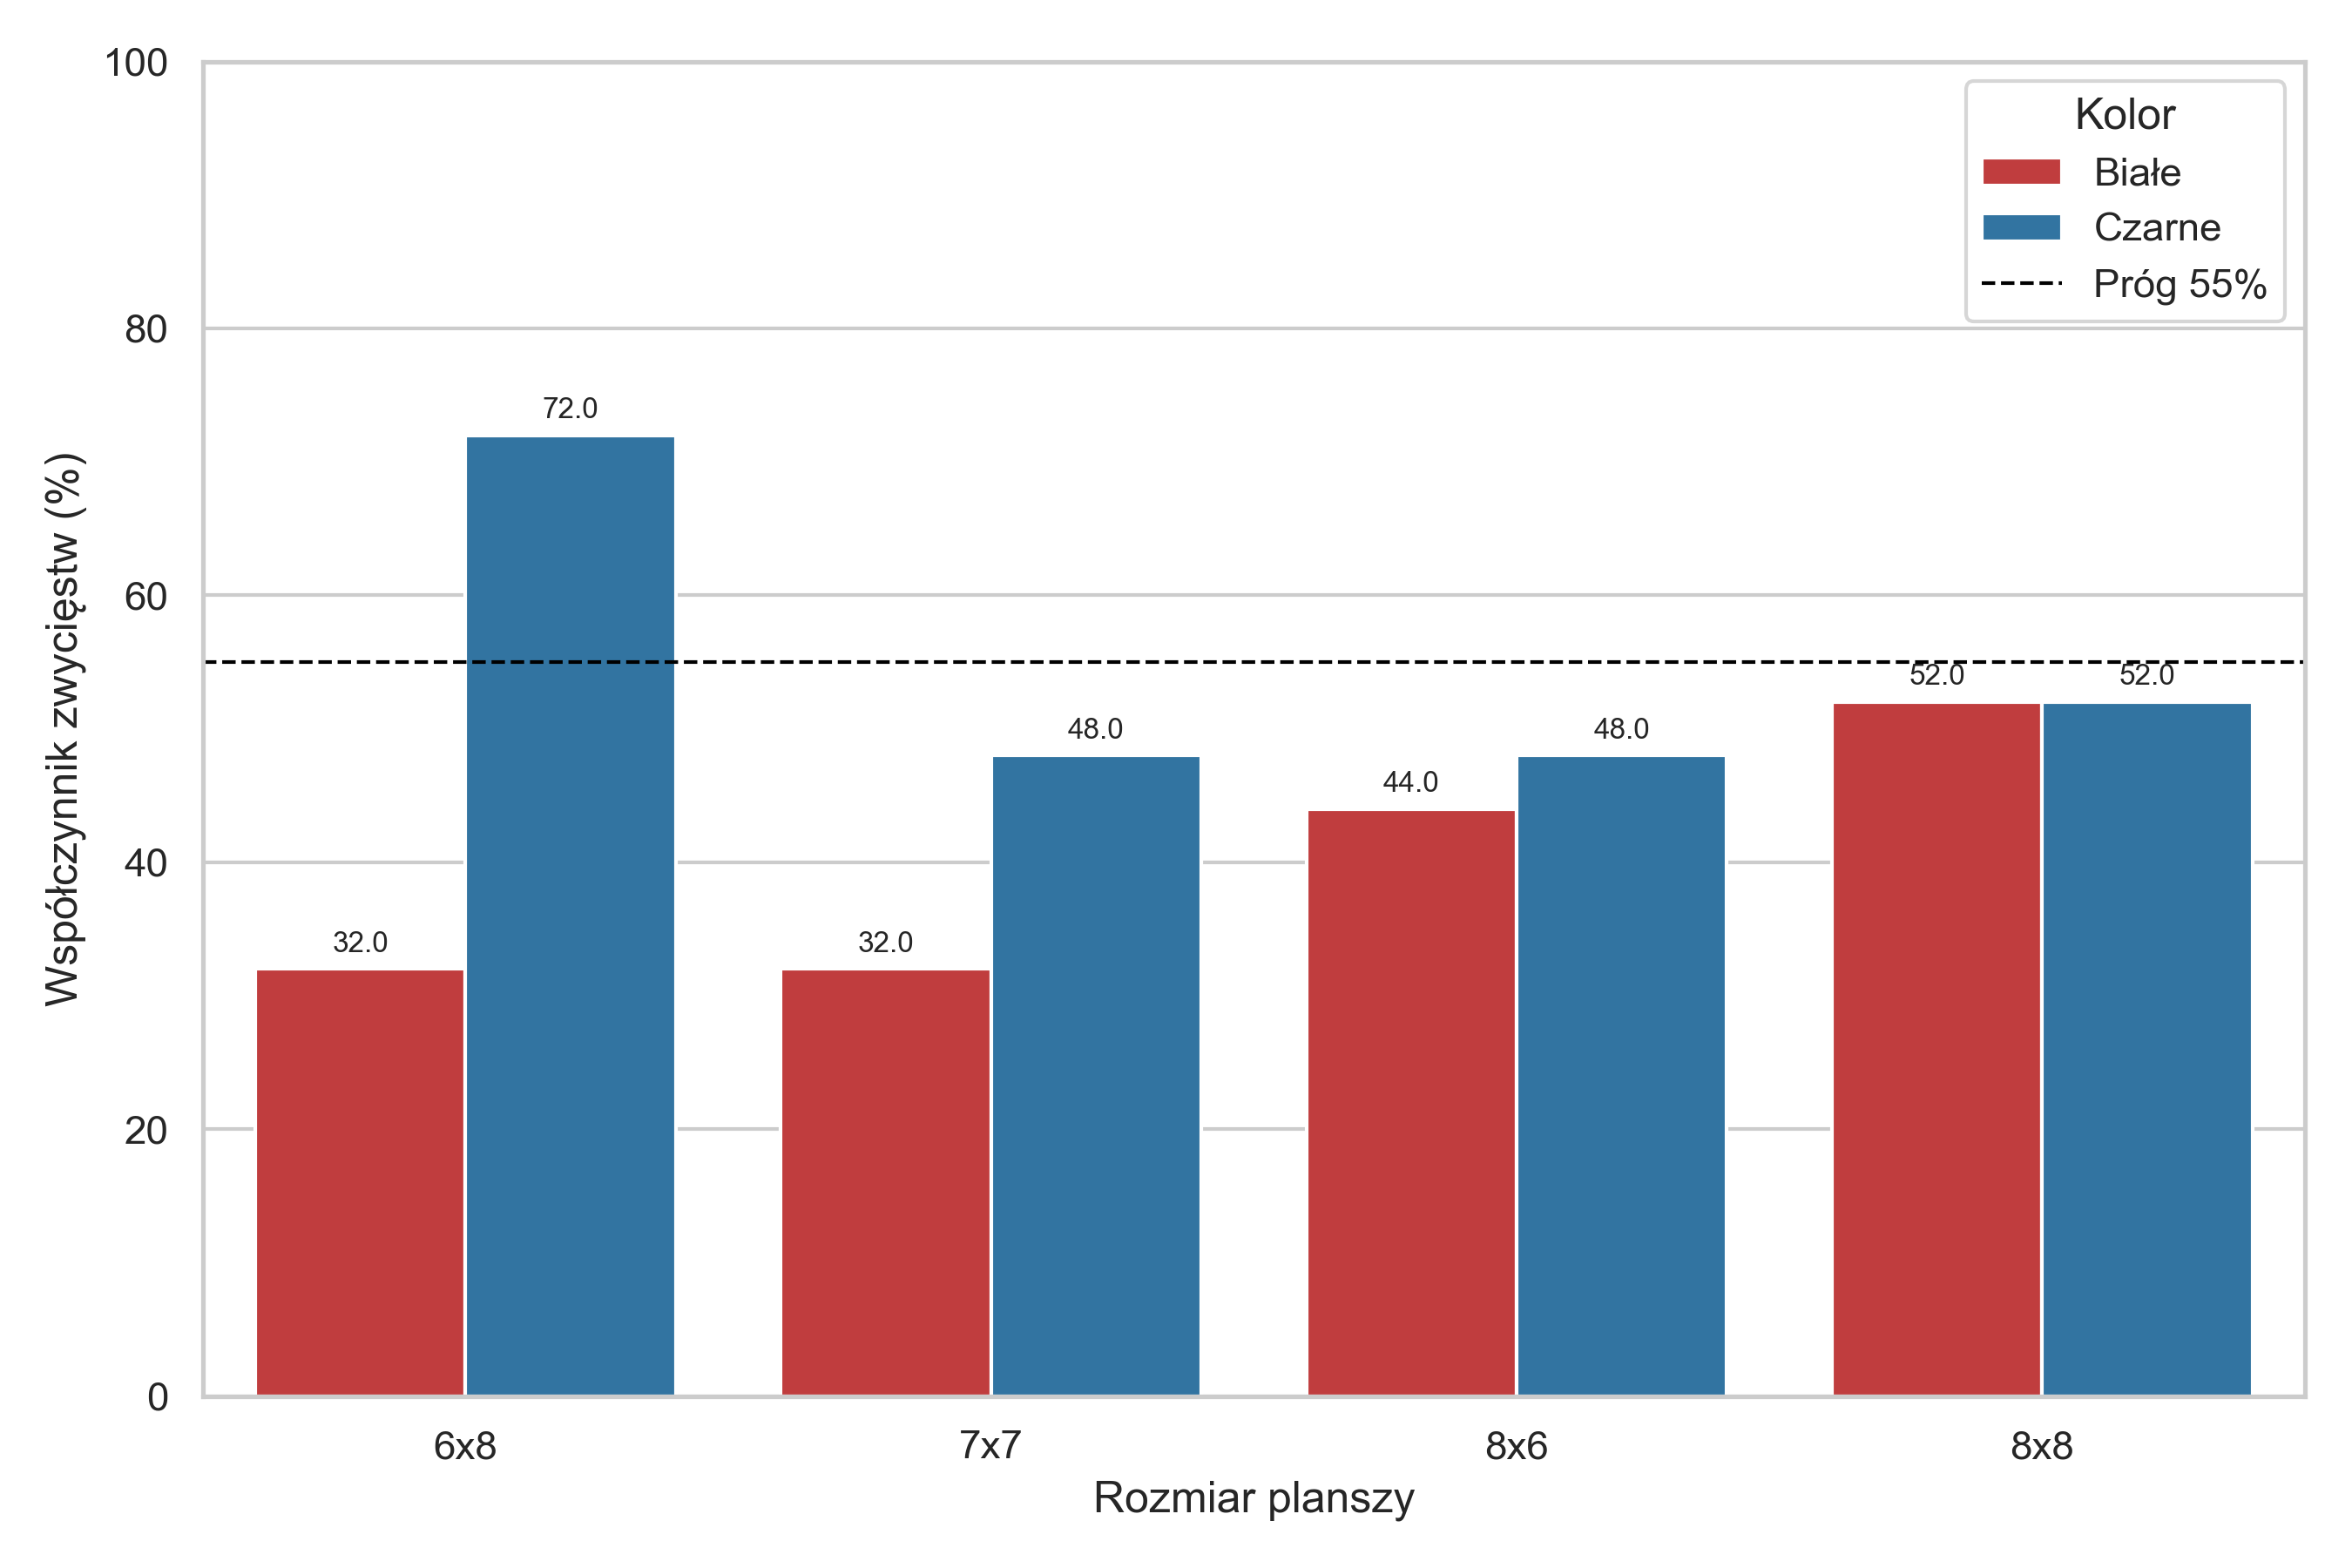
\includegraphics[width=0.92\textwidth]{images/h1_rave_win_rate_by_board_and_color.png}

        \vspace{0.05cm}
        {\scriptsize Wyniki z podziałem na kolor}
    \end{minipage}

    \vspace{0.2cm}

    \small
    \begin{itemize}
        \item MCTS + RAVE wygrał 95 z 200 partii, czyli 47.5\%.
        \item W żadnym rozmiarze planszy wynik nie przekroczył progu 55\%.
        \item Hipoteza H1 została odrzucona: AMAF nie poprawił stabilnie decyzji względem klasycznego MCTS.
    \end{itemize}
\end{frame}

\begin{frame}{Wpływ Heavy Playouts na MCTS -- metodologia}
    \begin{columns}[T]
    \begin{column}{0.52\textwidth}
        \structure{\textbf{Cel eksperymentu}}
        \vspace{0.1cm}
        \begin{itemize}
            \item Bezpośrednie porównanie MCTS + Heavy Playouts z klasycznym MCTS.
            \item Kryterium sukcesu: ponad 55\% zwycięstw wariantu heurystycznego.
            \item Heavy Playouts używa droższej, ale bardziej informacyjnej symulacji.
        \end{itemize}
    \end{column}

    \begin{column}{0.43\textwidth}
        \structure{\textbf{Limit czasu}}
        \vspace{0.1cm}
        \begin{itemize}
            \item Zastosowano limit 250 ms na ruch.
            \item Obaj agenci mieli taki sam budżet czasowy.
            \item Limit czasu jest ważniejszy niż stała liczba iteracji, bo pojedynczy playout jest wolniejszy.
        \end{itemize}
    \end{column}
    \end{columns}

    \vspace{0.35cm}

    \structure{\textbf{Zakres testów}}
    \begin{itemize}
        \item Plansze: $6 \times 8$, $7 \times 7$, $8 \times 6$, $8 \times 8$.
        \item 40 partii na każdy rozmiar planszy: 20 jako białe i 20 jako czarne.
        \item Strategia symulacji: $\epsilon$-greedy z $\epsilon = 0.1$.
    \end{itemize}
\end{frame}

\begin{frame}{Wpływ Heavy Playouts na MCTS -- wyniki}
    \centering
    \begin{minipage}{0.48\textwidth}
        \centering
        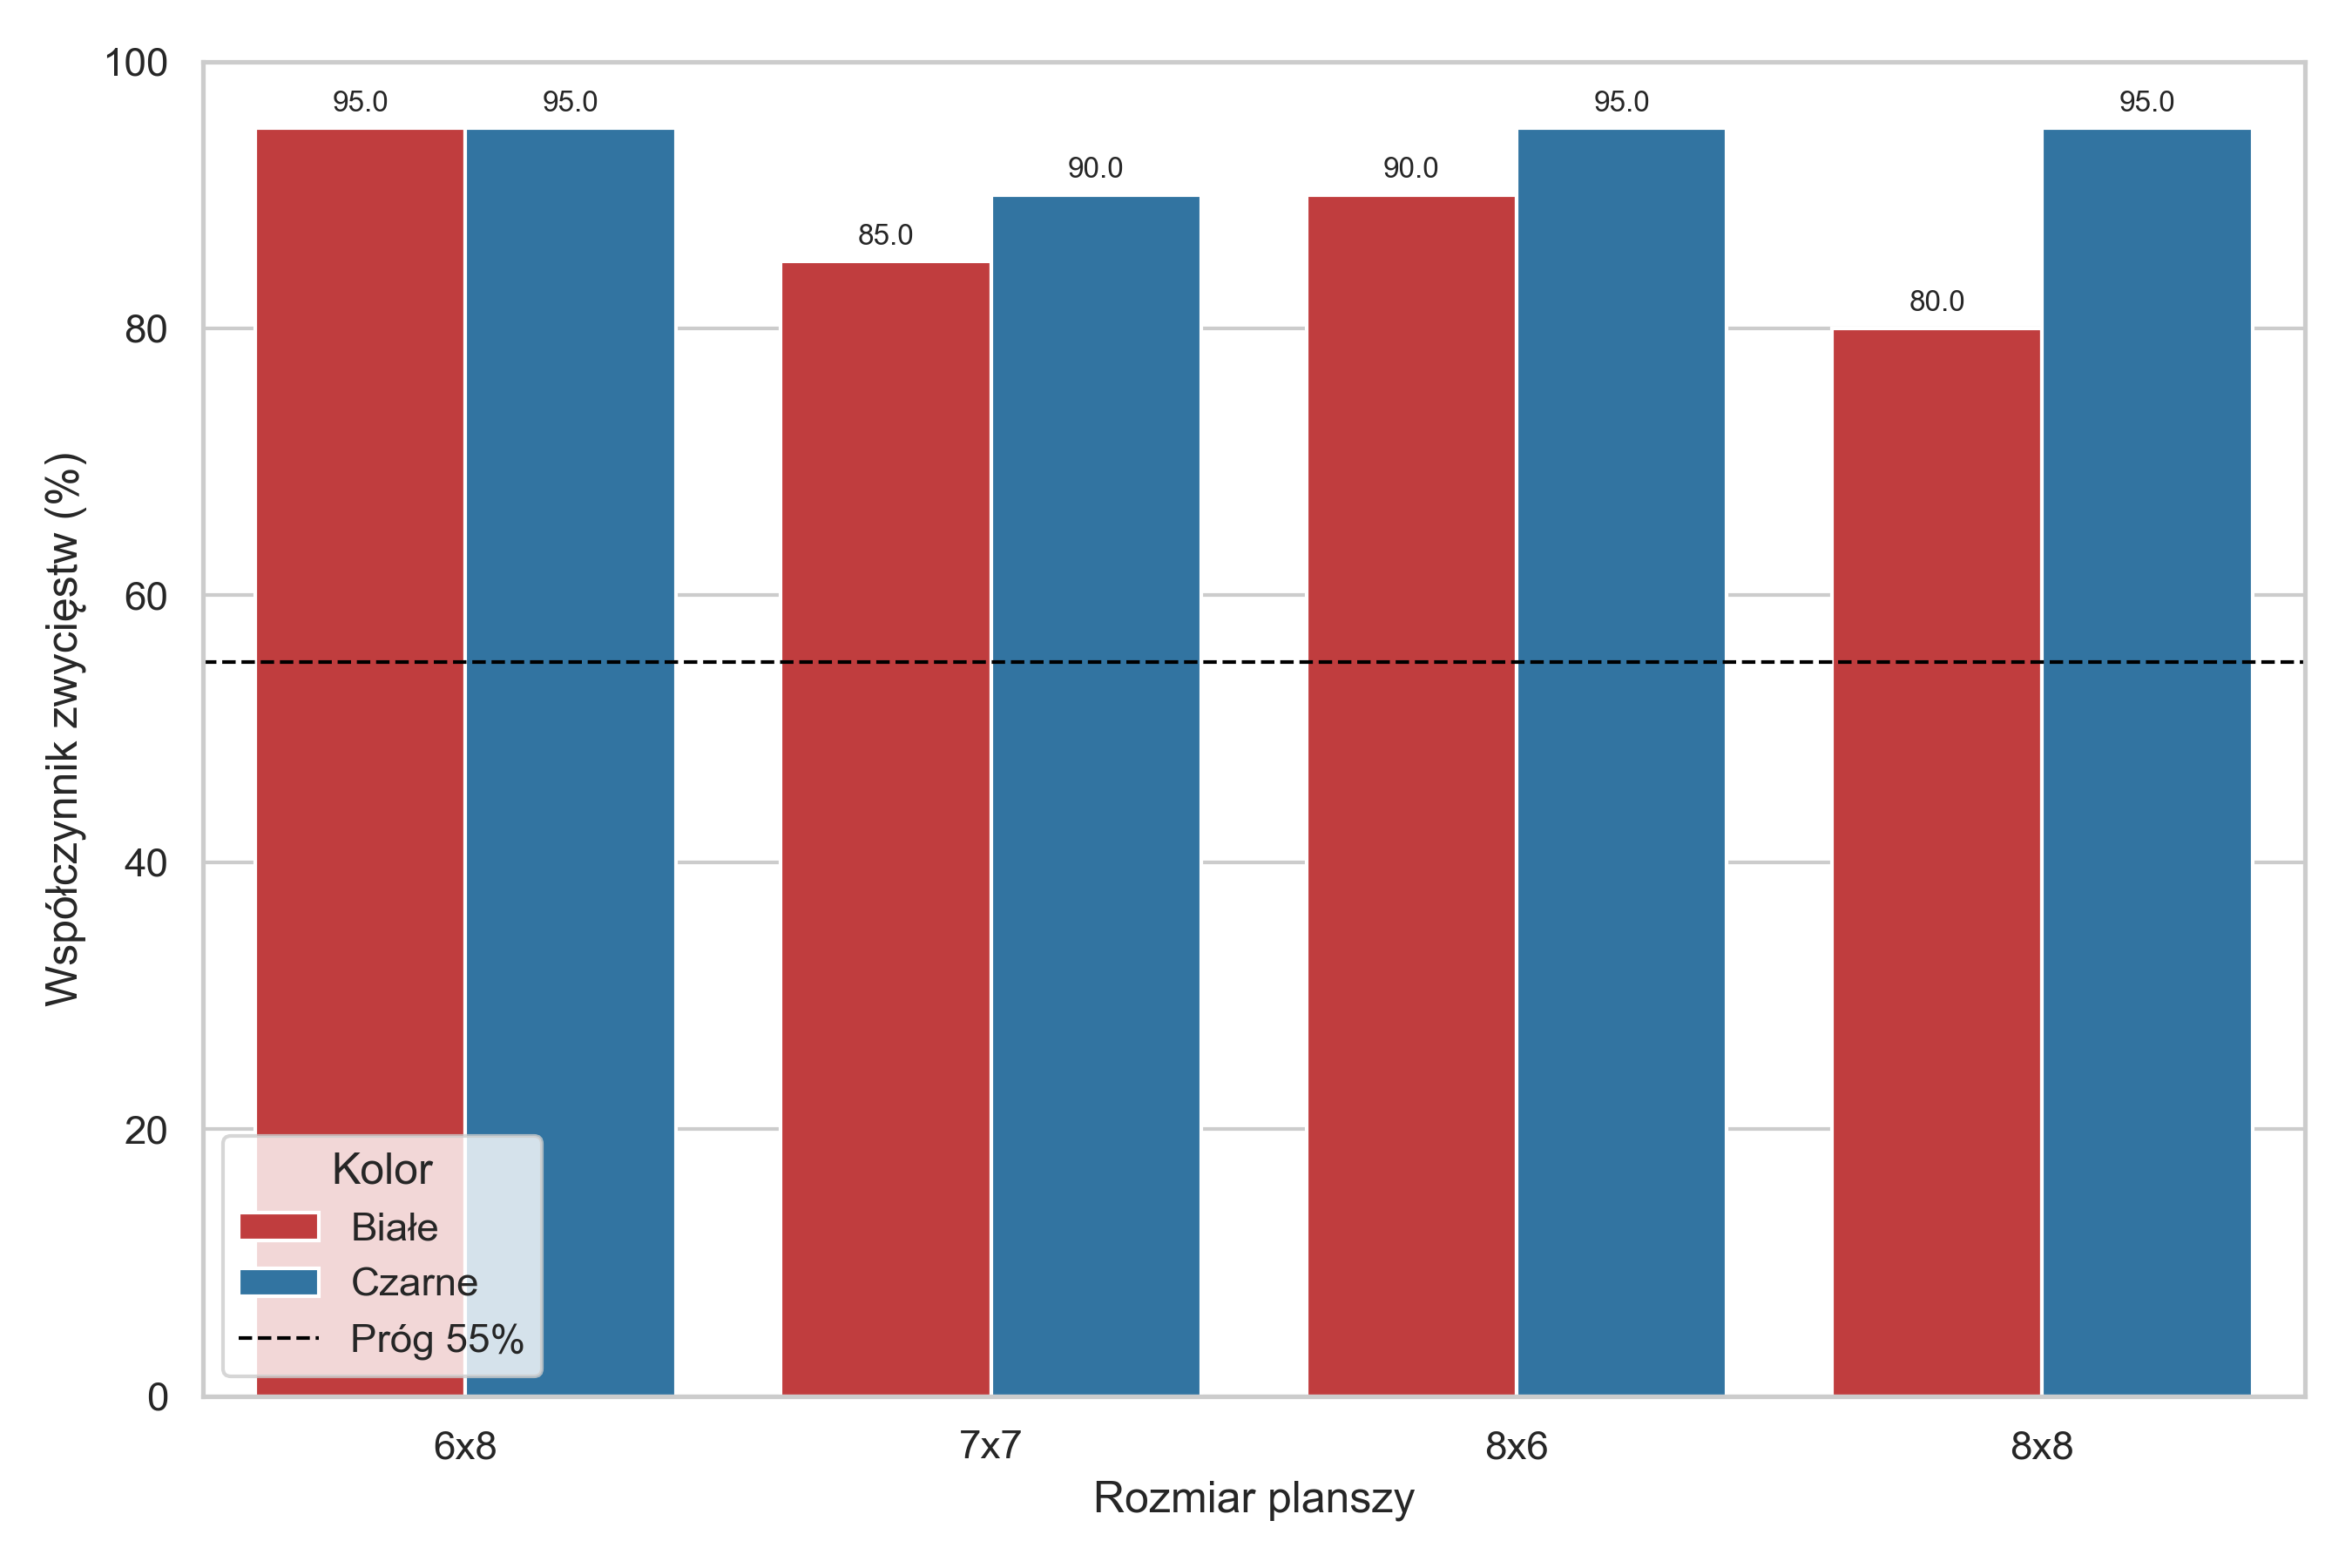
\includegraphics[width=0.92\textwidth]{images/h2_heavyplayouts_win_rate_by_board_and_color.png}

        \vspace{0.05cm}
        {\scriptsize Skuteczność z podziałem na kolor}
    \end{minipage}
    \hfill
    \begin{minipage}{0.48\textwidth}
        \centering
        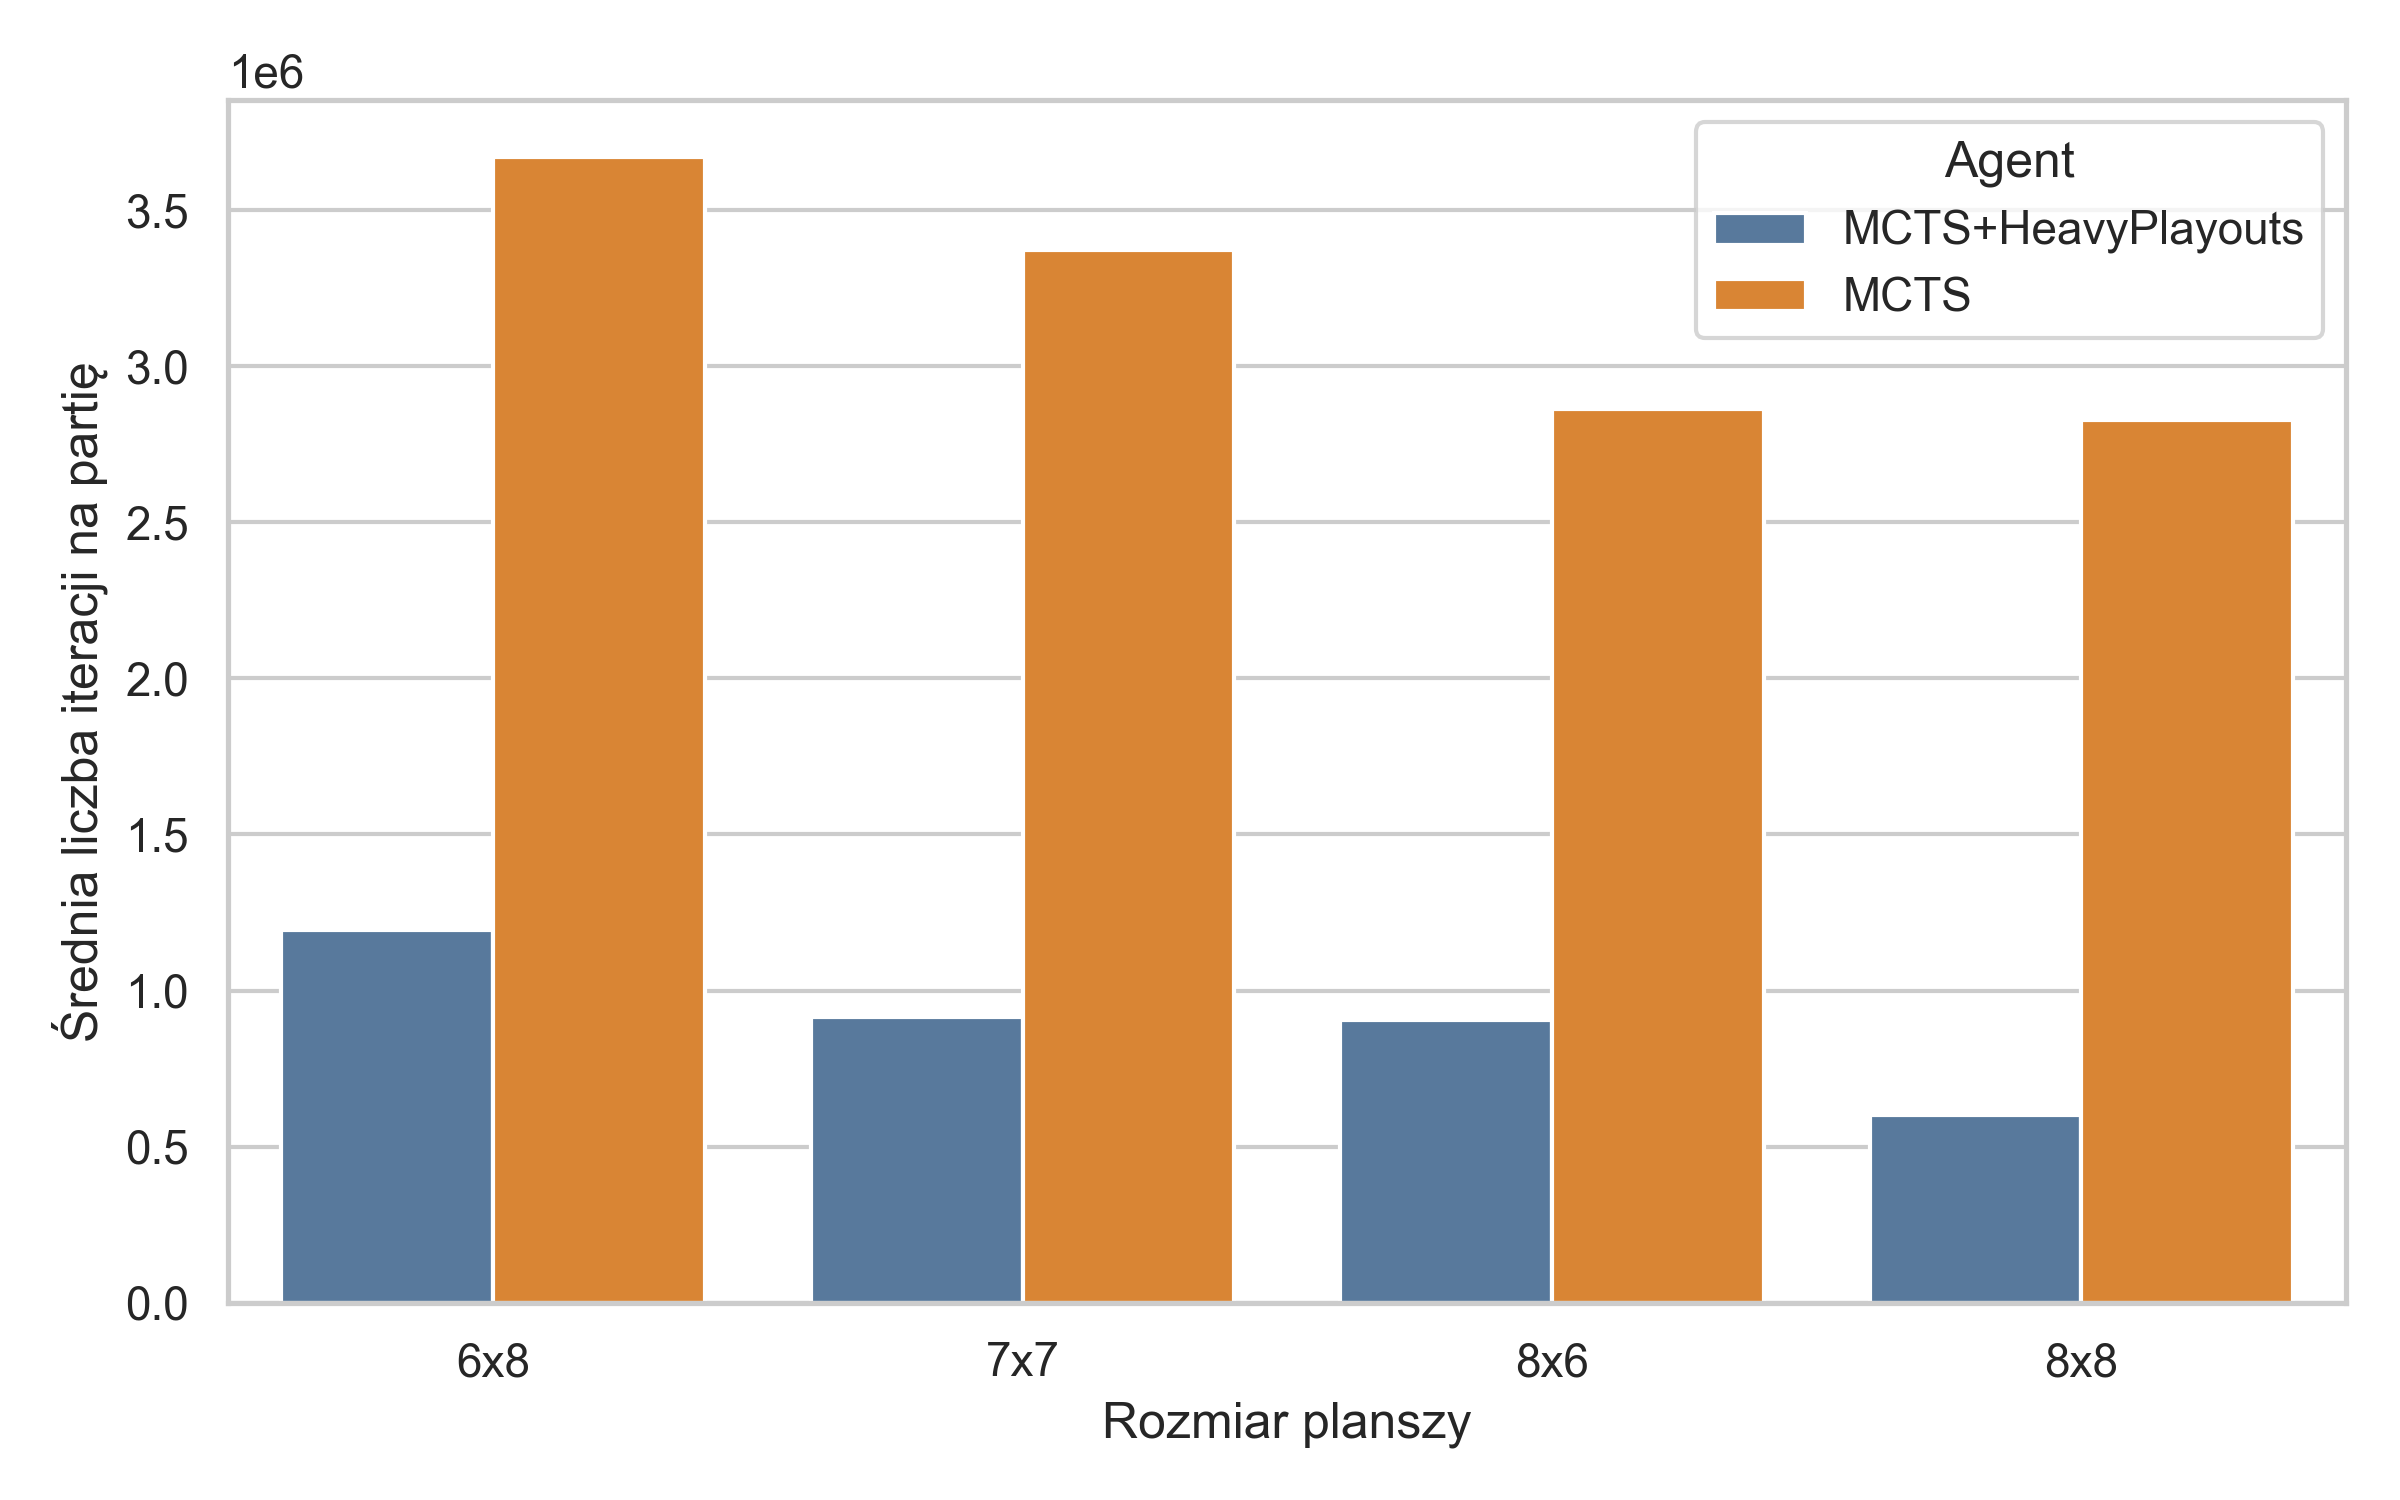
\includegraphics[width=0.92\textwidth]{images/h2_iterations_by_board.png}

        \vspace{0.05cm}
        {\scriptsize Liczba iteracji w limicie 250 ms}
    \end{minipage}

    \vspace{0.2cm}

    \small
    \begin{itemize}
        \item Heavy Playouts wygrał 145 ze 160 partii, czyli 90.6\%.
        \item Agent wykonywał mniej iteracji niż klasyczny MCTS, ale każda symulacja dawała lepszą informację.
        \item Hipoteza H2 została przyjęta: wiedza dziedzinowa w playoutach wyraźnie poprawiła decyzje.
    \end{itemize}
\end{frame}

\section{Interfejs graficzny}

\begin{frame}{Menu i rozgrywka}

\centering

\begin{minipage}{0.48\textwidth}
    \centering
    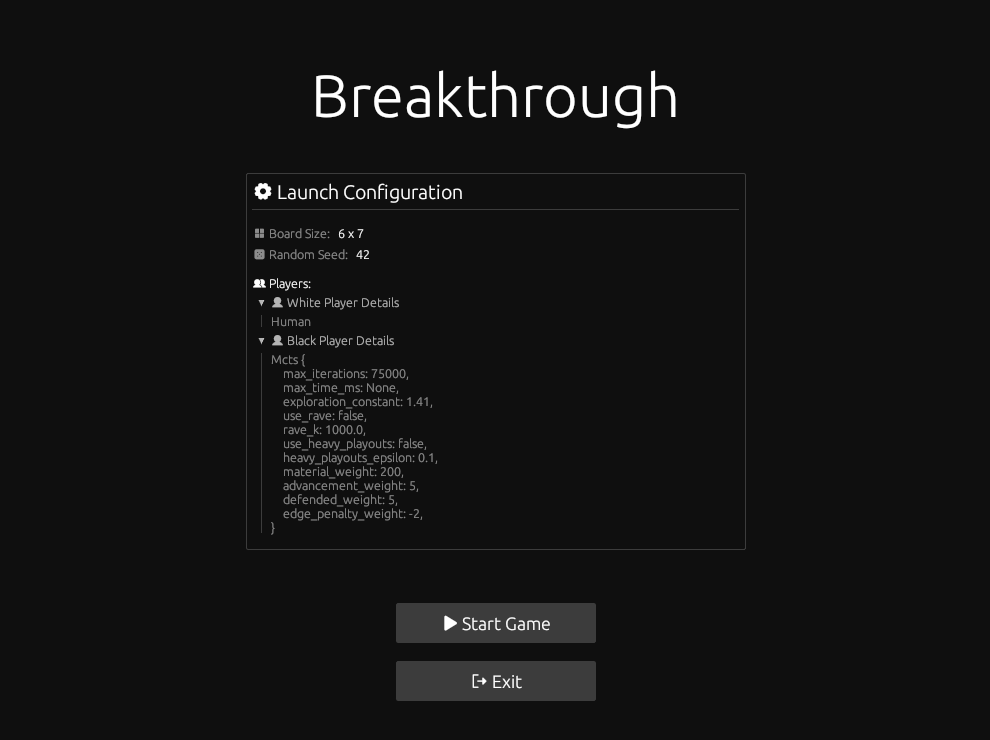
\includegraphics[width=\textwidth]{images/main_menu.png}

    \vspace{0.2cm}
    { Ekran startowy }
\end{minipage}
\hfill
\begin{minipage}{0.48\textwidth}
    \centering
    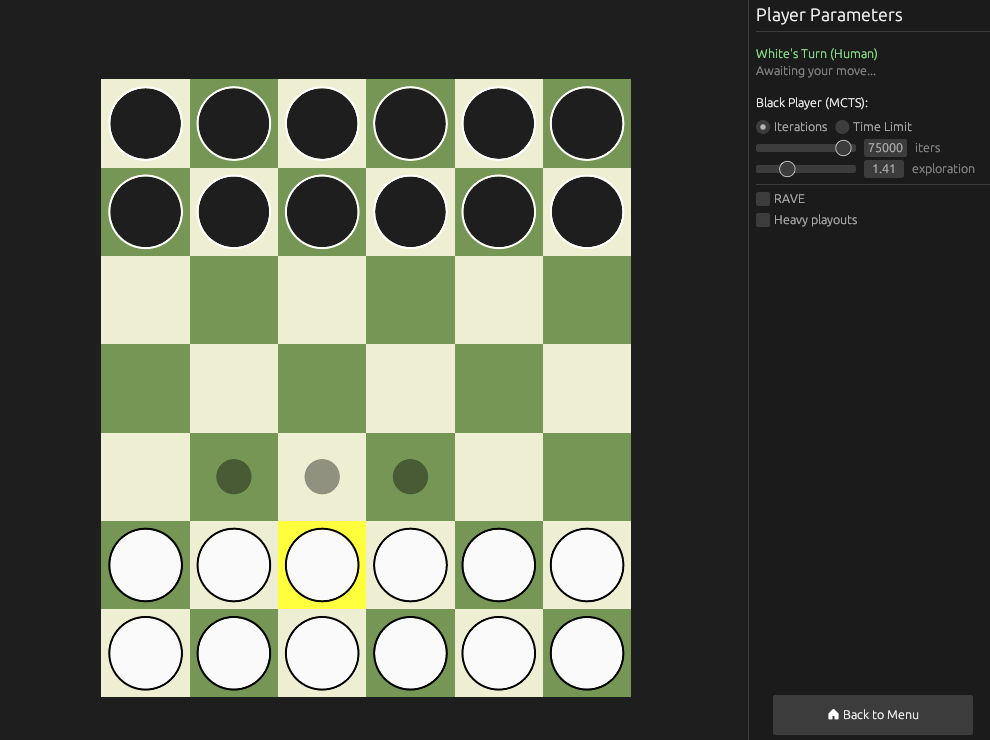
\includegraphics[width=\textwidth]{images/human_turn.png}

    \vspace{0.2cm}
    { Oczekiwanie na ruch gracza }
\end{minipage}

\end{frame}

\begin{frame}{Ruch agenta i koniec gry }

\centering

\begin{minipage}{0.48\textwidth}
    \centering
    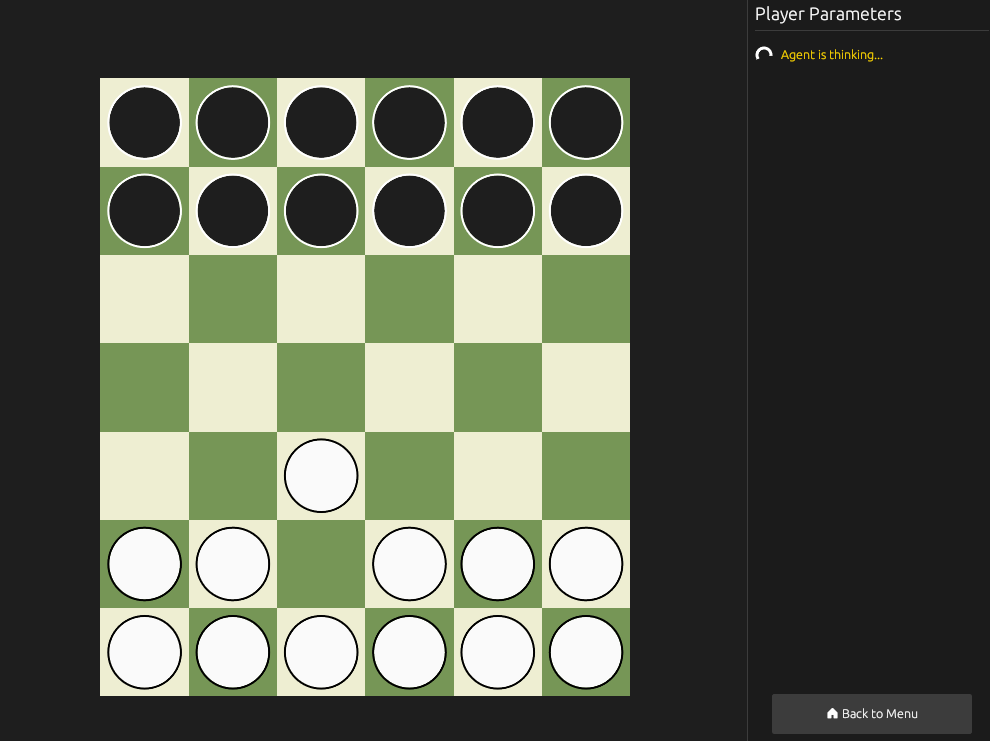
\includegraphics[width=\textwidth]{images/mcts_turn.png}

    \vspace{0.2cm}
    { Oczekiwanie na ruch agenta }
\end{minipage}
\hfill
\begin{minipage}{0.48\textwidth}
    \centering
    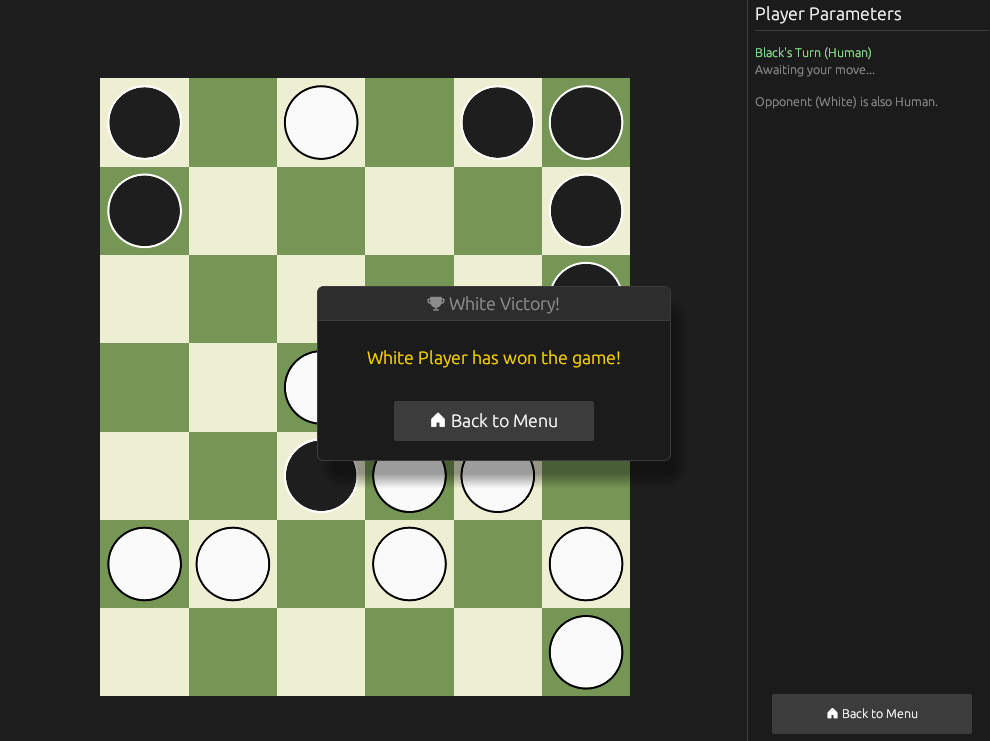
\includegraphics[width=\textwidth]{images/player_won.png}

    \vspace{0.2cm}
    { Ekran końcowy }
\end{minipage}

\end{frame}

\section{Testy z udziałem ludzi}

\begin{frame}{Tryb ślepego testu}

\centering

\begin{minipage}{0.48\textwidth}
    \centering
    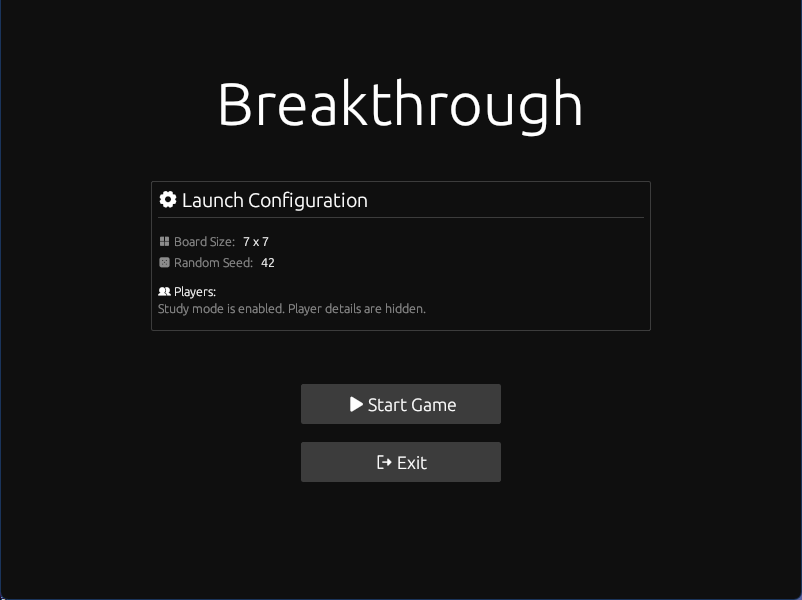
\includegraphics[width=0.94\textwidth]{images/blind_mode_welcome_screen.png}

    \vspace{0.1cm}
    {\scriptsize Ekran startowy bez nazwy agenta}
\end{minipage}
\hfill
\begin{minipage}{0.48\textwidth}
    \centering
    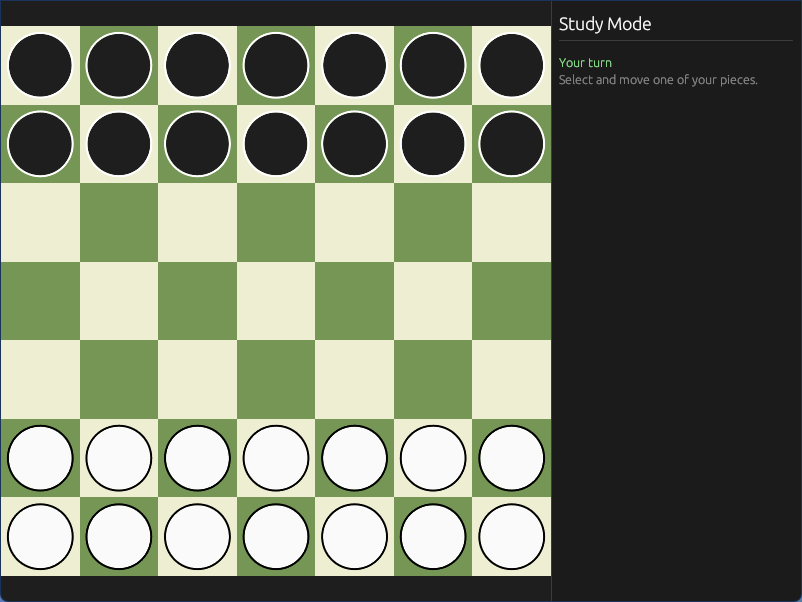
\includegraphics[width=0.94\textwidth]{images/blind_mode_board.png}

    \vspace{0.1cm}
    {\scriptsize Rozgrywka z ukrytym typem przeciwnika}
\end{minipage}

\vspace{0.2cm}

\small
\begin{itemize}
    \item Badani nie widzieli, czy grają przeciwko Minimax, MCTS, RAVE czy Heavy Playouts.
    \item Celem było oddzielenie realnej skuteczności agenta od sugestii wynikającej z jego nazwy.
\end{itemize}

\end{frame}

\begin{frame}{Wyniki testów z udziałem ludzi}

\centering

\begin{minipage}{0.48\textwidth}
    \centering
    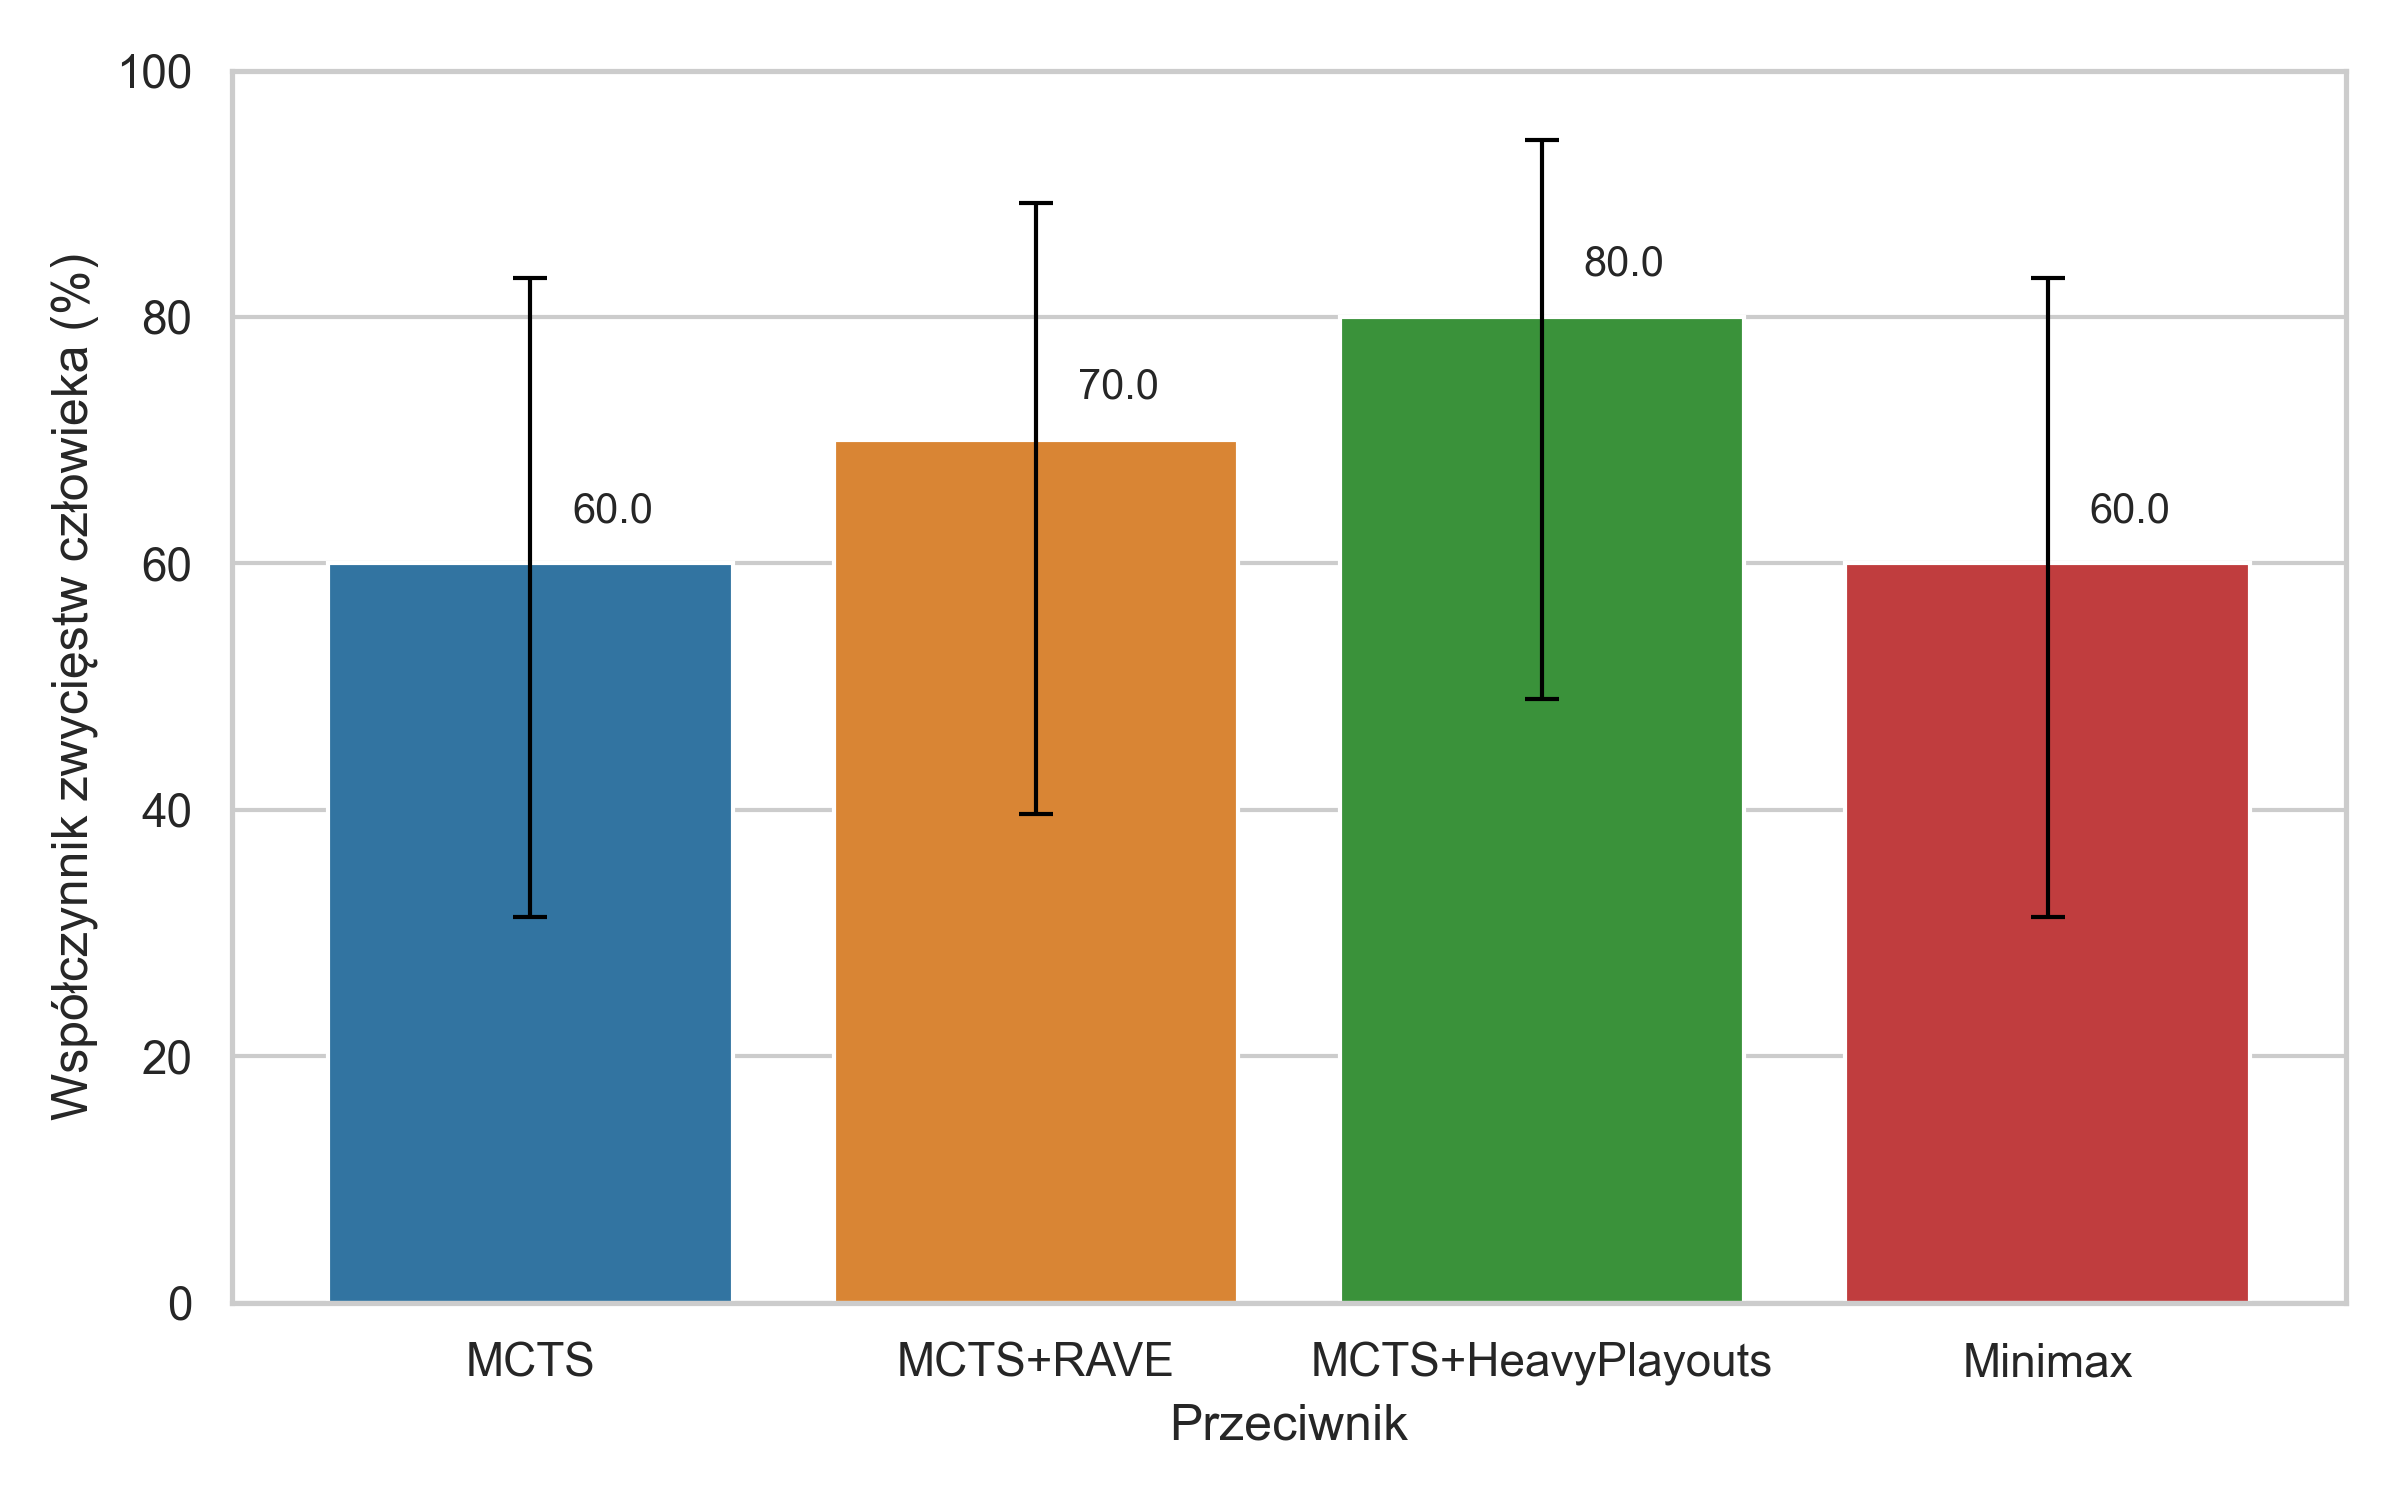
\includegraphics[width=\textwidth]{images/human_win_rate_by_agent.png}

    \vspace{0.15cm}
    {\scriptsize Współczynnik zwycięstw ludzi}
\end{minipage}
\hfill
\begin{minipage}{0.48\textwidth}
    \centering
    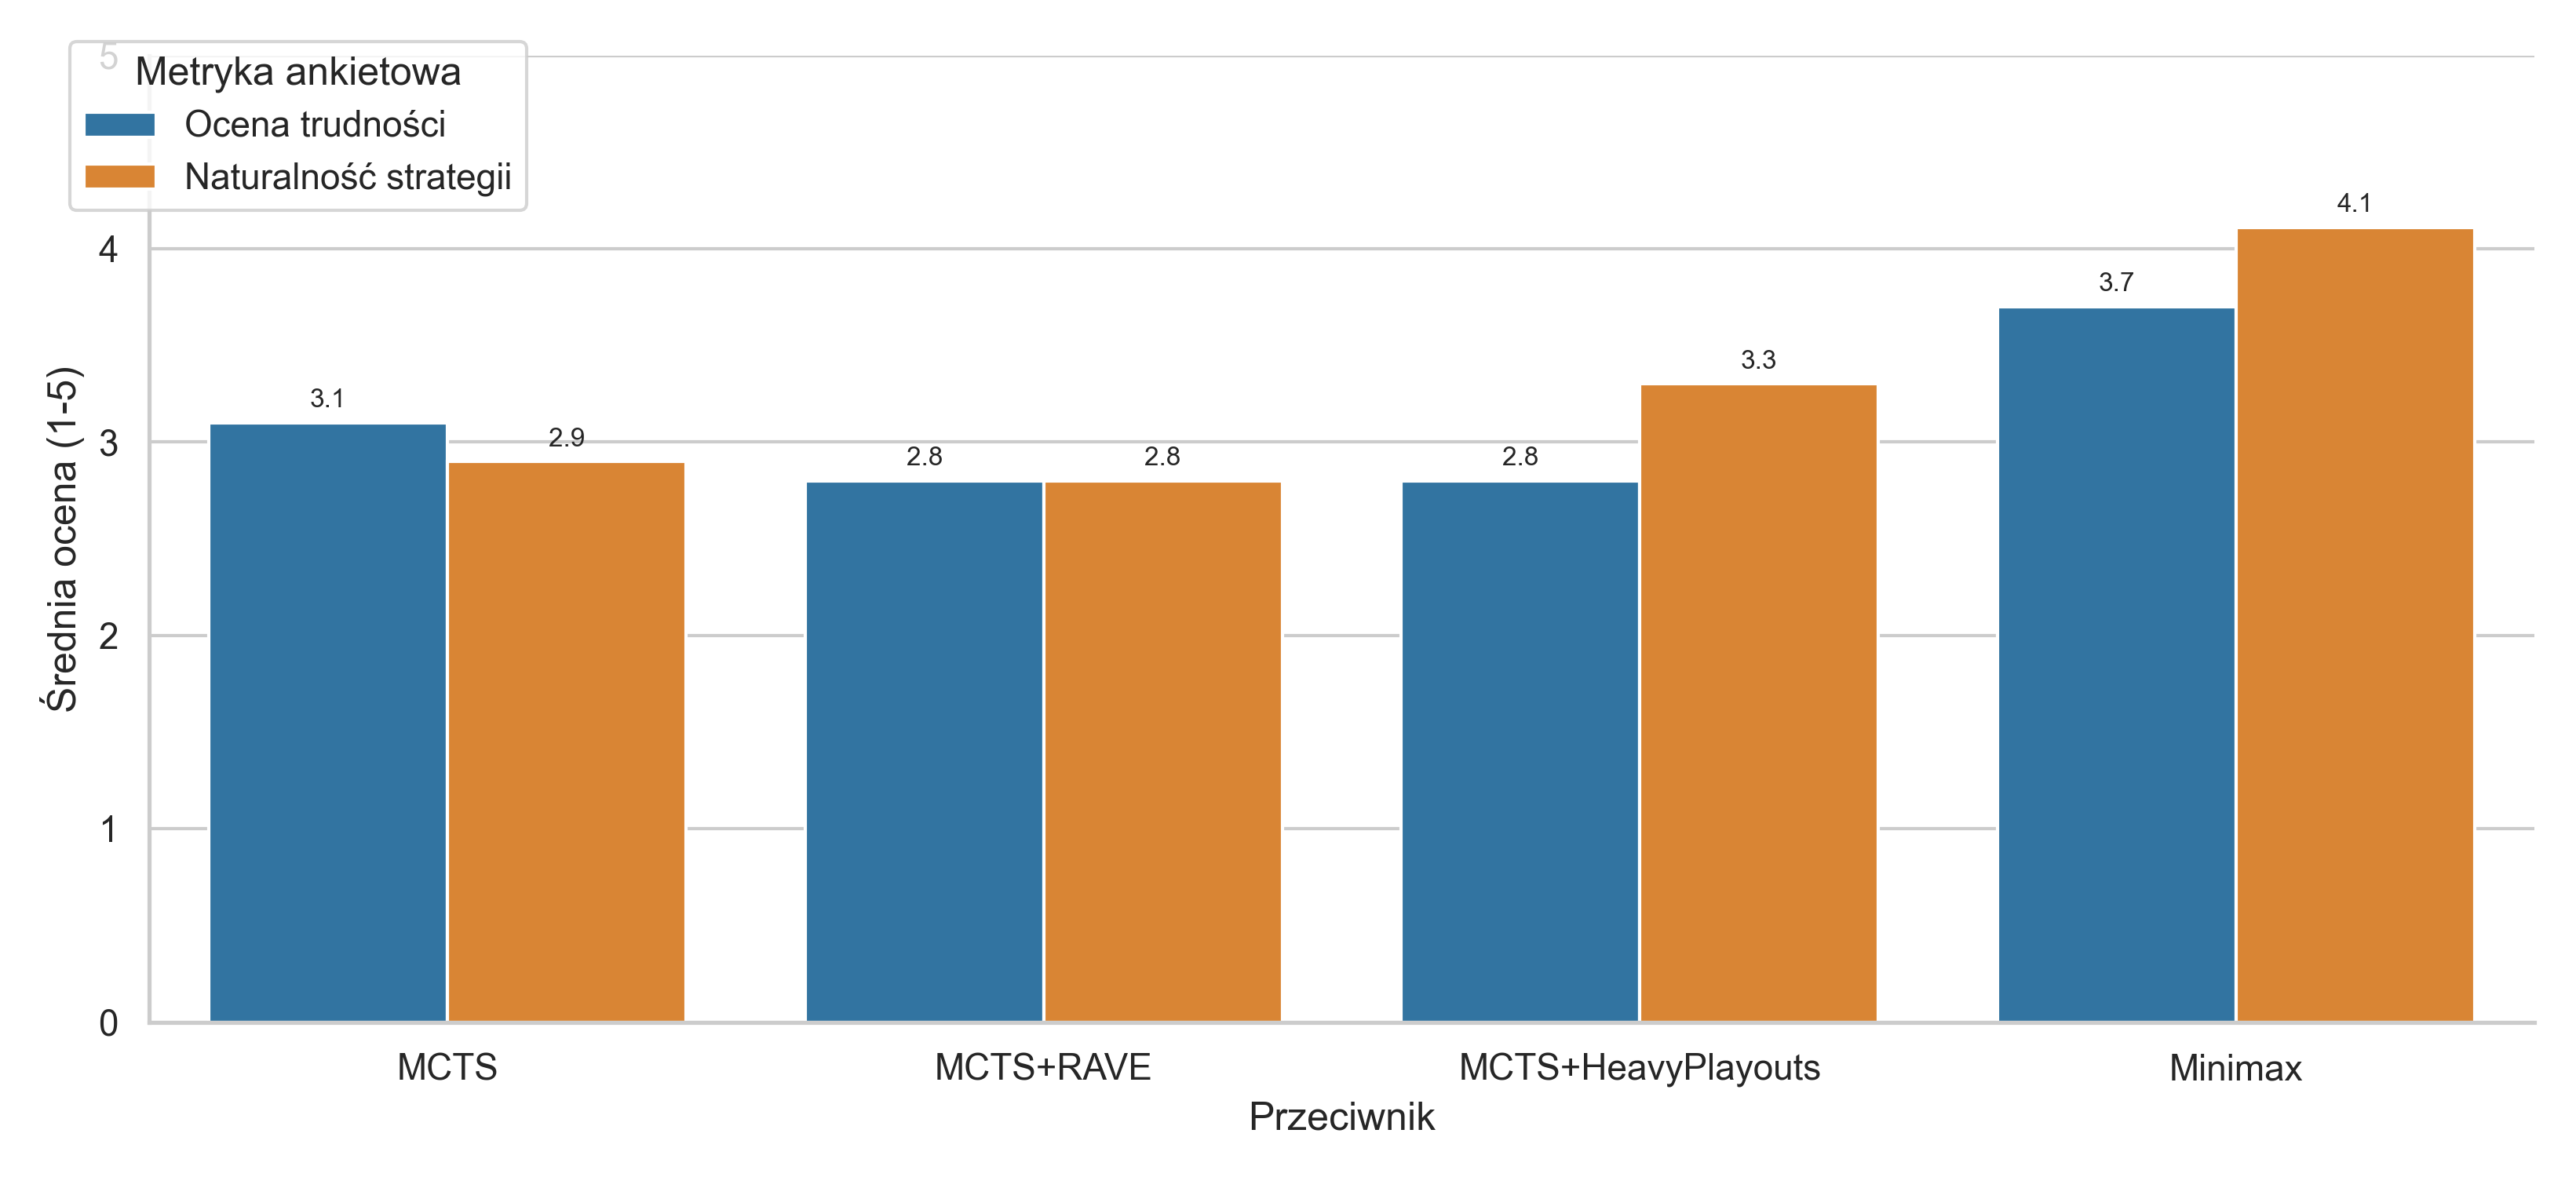
\includegraphics[width=\textwidth]{images/human_survey_ratings_by_agent.png}

    \vspace{0.15cm}
    {\scriptsize Ocena trudności i naturalności strategii}
\end{minipage}

\vspace{0.35cm}

\begin{itemize}
    \item Agenty grały sensownie, ale w testach nadal były słabsze od ludzi.
    \item Minimax był odbierany jako najbardziej naturalny i najtrudniejszy przeciwnik.
\end{itemize}

\end{frame}

\section{Bibliografia}

\begin{frame}[allowframebreaks]{Literatura}
    \scriptsize
    \begin{thebibliography}{99}

    \bibitem{coulom2006efficient}
    R. Coulom, 
    \textit{Efficient Selectivity and Backup Operators in Monte-Carlo Tree Search}, 
    w: \textit{Computers and Games}, 
    Springer, Berlin, Heidelberg, 2006, s. 72--83.
    
    \bibitem{kocsis2006bandit}
    L. Kocsis, C. Szepesv{\'a}ri, 
    \textit{Bandit Based Monte-Carlo Planning}, 
    w: \textit{Machine Learning: ECML 2006}, 
    Springer, Berlin, Heidelberg, 2006, s. 282--293.
    
    \bibitem{saffidine2012solving}
    A. Saffidine, N. Jouandeau, and T. Cazenave, 
    \textit{Solving Breakthrough with Race Patterns and Job-Level Proof Number Search}, 
    w: \textit{Advances in Computer Games}, 
    Springer, Berlin, Heidelberg, 2012, s. 236--247.
    
    \bibitem{browne2012survey}
    C. B. Browne i in., 
    \textit{A Survey of Monte Carlo Tree Search Methods}, 
    w: \textit{IEEE Transactions on Computational Intelligence and AI in Games}, 
    vol. 4, no. 1, 2012, s. 1--43.
    
    \bibitem{russell2010artificial}
    S. J. Russell, P. Norvig, 
    \textit{Artificial Intelligence: A Modern Approach}, 
    3rd ed., Prentice Hall, 2010.
    
    \bibitem{gelly2007monte}
    S. Gelly, D. Silver, 
    \textit{Monte-Carlo tree search and rapid action value estimation in computer Go}, 
    w: \textit{Proceedings of the 24th international conference on Machine learning (ICML '07)}, 
    ACM, New York, 2007, s. 273--280.
    
    \bibitem{sutton2018reinforcement}
    R. S. Sutton, A. G. Barto, 
    \textit{Reinforcement Learning: An Introduction}, 
    2nd ed., MIT Press, Cambridge, MA, 2018.
    
    \bibitem{knuth1975alpha}
    D. E. Knuth, R. W. Moore, 
    \textit{An Analysis of Alpha-Beta Pruning}, 
    w: \textit{Artificial Intelligence}, vol. 6, no. 4, 1975, s. 293--326.
    
    \bibitem{rust_lang}
    Klabnik, S., \& Nichols, C. (2023). 
    \textit{The Rust Programming Language}. 
    No Starch Press. \\
    Dostępne pod adresem: \url{https://www.rust-lang.org/}
    
    \bibitem{python_lang}
    Python Software Foundation (2026). 
    \textit{Python 3 Reference Manual}. \\
    Dostępne pod adresem: \url{https://www.python.org/}

    \end{thebibliography}
\end{frame}

\begin{frame}[standout]
    Dziękujemy za uwagę!
\end{frame}

\end{document}
